%% *****************************************************************************
%% A Comprehensive Survey on Software Defined Networking
%% 
%% Diego Kreutz, Fernando Ramos, Paulo Verissimo,
%% Christian Esteve Rothenberg, Siamak Azodolmolky, Steve Uhlig
%%
%% Submission: DD/MM/2014
%% Revised on: DD/MM/2014
%% Final version: DD/MM/2014
%% *****************************************************************************
%%
%% bare_jrnl.tex
%% V1.4
%% 2012/12/27
%% by Michael Shell
%% see http://www.michaelshell.org/
%% for current contact information.
%%
%% This is a skeleton file demonstrating the use of IEEEtran.cls
%% (requires IEEEtran.cls version 1.8 or later) with an IEEE journal paper.
%%
%% Support sites:
%% http://www.michaelshell.org/tex/ieeetran/
%% http://www.ctan.org/tex-archive/macros/latex/contrib/IEEEtran/
%% and
%% http://www.ieee.org/

% *** Authors should verify (and, if needed, correct) their LaTeX system  ***
% *** with the testflow diagnostic prior to trusting their LaTeX platform ***
% *** with production work. IEEE's font choices can trigger bugs that do  ***
% *** not appear when using other class files.                            ***
% The testflow support page is at:
% http://www.michaelshell.org/tex/testflow/

%%*************************************************************************
%% Legal Notice:
%% This code is offered as-is without any warranty either expressed or
%% implied; without even the implied warranty of MERCHANTABILITY or
%% FITNESS FOR A PARTICULAR PURPOSE! 
%% User assumes all risk.
%% In no event shall IEEE or any contributor to this code be liable for
%% any damages or losses, including, but not limited to, incidental,
%% consequential, or any other damages, resulting from the use or misuse
%% of any information contained here.
%%
%% All comments are the opinions of their respective authors and are not
%% necessarily endorsed by the IEEE.
%%
%% This work is distributed under the LaTeX Project Public License (LPPL)
%% ( http://www.latex-project.org/ ) version 1.3, and may be freely used,
%% distributed and modified. A copy of the LPPL, version 1.3, is included
%% in the base LaTeX documentation of all distributions of LaTeX released
%% 2003/12/01 or later.
%% Retain all contribution notices and credits.
%% ** Modified files should be clearly indicated as such, including  **
%% ** renaming them and changing author support contact information. **
%%
%% File list of work: IEEEtran.cls, IEEEtran_HOWTO.pdf, bare_adv.tex,
%%                    bare_conf.tex, bare_jrnl.tex, bare_jrnl_compsoc.tex,
%%                    bare_jrnl_transmag.tex
%%*************************************************************************

% Note that the a4paper option is mainly intended so that authors in
% countries using A4 can easily print to A4 and see how their papers will
% look in print - the typesetting of the document will not typically be
% affected with changes in paper size (but the bottom and side margins will).
% Use the testflow package mentioned above to verify correct handling of
% both paper sizes by the user's LaTeX system.
%
% Also note that the "draftcls" or "draftclsnofoot", not "draft", option
% should be used if it is desired that the figures are to be displayed in
% draft mode.
%
\documentclass[journal]{IEEEtran}
%
% If IEEEtran.cls has not been installed into the LaTeX system files,
% manually specify the path to it like:
% \documentclass[journal]{../sty/IEEEtran}

\usepackage{epsfig}
\usepackage{graphicx}
%\usepackage{url}
\usepackage[hyphens]{url}
%\ifpdf
%\usepackage[breaklinks=true,pdfborder={0 0 0},bookmarksopen]{hyperref}
%\else
%\usepackage[pdfborder={0 0 0},bookmarksopen]{hyperref}
%\usepackage[hyphenbreaks]{breakurl}
%\fi
\usepackage{xspace}
\usepackage{array}
\usepackage{tabularx}
\usepackage{color}
\usepackage{makeidx}
\usepackage[colorlinks=true,urlcolor=SteelBlue4,linkcolor=Firebrick4,hyperindex,breaklinks]{hyperref}
\usepackage[hyphenbreaks]{breakurl}
\usepackage[table,hyperref,x11names]{xcolor}
\usepackage{multirow}
\usepackage{comment}

%\usepackage[show]{chato-notes}
\usepackage[hide]{chato-notes}

% Some very useful LaTeX packages include:
% (uncomment the ones you want to load)


% *** MISC UTILITY PACKAGES ***
%
%\usepackage{ifpdf}
% Heiko Oberdiek's ifpdf.sty is very useful if you need conditional
% compilation based on whether the output is pdf or dvi.
% usage:
% \ifpdf
%   % pdf code
% \else
%   % dvi code
% \fi
% The latest version of ifpdf.sty can be obtained from:
% http://www.ctan.org/tex-archive/macros/latex/contrib/oberdiek/
% Also, note that IEEEtran.cls V1.7 and later provides a builtin
% \ifCLASSINFOpdf conditional that works the same way.
% When switching from latex to pdflatex and vice-versa, the compiler may
% have to be run twice to clear warning/error messages.






% *** CITATION PACKAGES ***
%
%\usepackage{cite}
% cite.sty was written by Donald Arseneau
% V1.6 and later of IEEEtran pre-defines the format of the cite.sty package
% \cite{} output to follow that of IEEE. Loading the cite package will
% result in citation numbers being automatically sorted and properly
% "compressed/ranged". e.g., [1], [9], [2], [7], [5], [6] without using
% cite.sty will become [1], [2], [5]--[7], [9] using cite.sty. cite.sty's
% \cite will automatically add leading space, if needed. Use cite.sty's
% noadjust option (cite.sty V3.8 and later) if you want to turn this off
% such as if a citation ever needs to be enclosed in parenthesis.
% cite.sty is already installed on most LaTeX systems. Be sure and use
% version 4.0 (2003-05-27) and later if using hyperref.sty. cite.sty does
% not currently provide for hyperlinked citations.
% The latest version can be obtained at:
% http://www.ctan.org/tex-archive/macros/latex/contrib/cite/
% The documentation is contained in the cite.sty file itself.






% *** GRAPHICS RELATED PACKAGES ***
%
\ifCLASSINFOpdf
  % \usepackage[pdftex]{graphicx}
  % declare the path(s) where your graphic files are
  % \graphicspath{{../pdf/}{../jpeg/}}
  % and their extensions so you won't have to specify these with
  % every instance of \includegraphics
  % \DeclareGraphicsExtensions{.pdf,.jpeg,.png}
\else
  % or other class option (dvipsone, dvipdf, if not using dvips). graphicx
  % will default to the driver specified in the system graphics.cfg if no
  % driver is specified.
  % \usepackage[dvips]{graphicx}
  % declare the path(s) where your graphic files are
  % \graphicspath{{../eps/}}
  % and their extensions so you won't have to specify these with
  % every instance of \includegraphics
  % \DeclareGraphicsExtensions{.eps}
\fi
% graphicx was written by David Carlisle and Sebastian Rahtz. It is
% required if you want graphics, photos, etc. graphicx.sty is already
% installed on most LaTeX systems. The latest version and documentation
% can be obtained at: 
% http://www.ctan.org/tex-archive/macros/latex/required/graphics/
% Another good source of documentation is "Using Imported Graphics in
% LaTeX2e" by Keith Reckdahl which can be found at:
% http://www.ctan.org/tex-archive/info/epslatex/
%
% latex, and pdflatex in dvi mode, support graphics in encapsulated
% postscript (.eps) format. pdflatex in pdf mode supports graphics
% in .pdf, .jpeg, .png and .mps (metapost) formats. Users should ensure
% that all non-photo figures use a vector format (.eps, .pdf, .mps) and
% not a bitmapped formats (.jpeg, .png). IEEE frowns on bitmapped formats
% which can result in "jaggedy"/blurry rendering of lines and letters as
% well as large increases in file sizes.
%
% You can find documentation about the pdfTeX application at:
% http://www.tug.org/applications/pdftex





% *** MATH PACKAGES ***
%
%\usepackage[cmex10]{amsmath}
% A popular package from the American Mathematical Society that provides
% many useful and powerful commands for dealing with mathematics. If using
% it, be sure to load this package with the cmex10 option to ensure that
% only type 1 fonts will utilized at all point sizes. Without this option,
% it is possible that some math symbols, particularly those within
% footnotes, will be rendered in bitmap form which will result in a
% document that can not be IEEE Xplore compliant!
%
% Also, note that the amsmath package sets \interdisplaylinepenalty to 10000
% thus preventing page breaks from occurring within multiline equations. Use:
%\interdisplaylinepenalty=2500
% after loading amsmath to restore such page breaks as IEEEtran.cls normally
% does. amsmath.sty is already installed on most LaTeX systems. The latest
% version and documentation can be obtained at:
% http://www.ctan.org/tex-archive/macros/latex/required/amslatex/math/





% *** SPECIALIZED LIST PACKAGES ***
%
%\usepackage{algorithmic}
% algorithmic.sty was written by Peter Williams and Rogerio Brito.
% This package provides an algorithmic environment fo describing algorithms.
% You can use the algorithmic environment in-text or within a figure
% environment to provide for a floating algorithm. Do NOT use the algorithm
% floating environment provided by algorithm.sty (by the same authors) or
% algorithm2e.sty (by Christophe Fiorio) as IEEE does not use dedicated
% algorithm float types and packages that provide these will not provide
% correct IEEE style captions. The latest version and documentation of
% algorithmic.sty can be obtained at:
% http://www.ctan.org/tex-archive/macros/latex/contrib/algorithms/
% There is also a support site at:
% http://algorithms.berlios.de/index.html
% Also of interest may be the (relatively newer and more customizable)
% algorithmicx.sty package by Szasz Janos:
% http://www.ctan.org/tex-archive/macros/latex/contrib/algorithmicx/




% *** ALIGNMENT PACKAGES ***
%
%\usepackage{array}
% Frank Mittelbach's and David Carlisle's array.sty patches and improves
% the standard LaTeX2e array and tabular environments to provide better
% appearance and additional user controls. As the default LaTeX2e table
% generation code is lacking to the point of almost being broken with
% respect to the quality of the end results, all users are strongly
% advised to use an enhanced (at the very least that provided by array.sty)
% set of table tools. array.sty is already installed on most systems. The
% latest version and documentation can be obtained at:
% http://www.ctan.org/tex-archive/macros/latex/required/tools/


% IEEEtran contains the IEEEeqnarray family of commands that can be used to
% generate multiline equations as well as matrices, tables, etc., of high
% quality.




% *** SUBFIGURE PACKAGES ***
%\ifCLASSOPTIONcompsoc
%  \usepackage[caption=false,font=normalsize,labelfont=sf,textfont=sf]{subfig}
%\else
%  \usepackage[caption=false,font=footnotesize]{subfig}
%\fi
% subfig.sty, written by Steven Douglas Cochran, is the modern replacement
% for subfigure.sty, the latter of which is no longer maintained and is
% incompatible with some LaTeX packages including fixltx2e. However,
% subfig.sty requires and automatically loads Axel Sommerfeldt's caption.sty
% which will override IEEEtran.cls' handling of captions and this will result
% in non-IEEE style figure/table captions. To prevent this problem, be sure
% and invoke subfig.sty's "caption=false" package option (available since
% subfig.sty version 1.3, 2005/06/28) as this is will preserve IEEEtran.cls
% handling of captions.
% Note that the Computer Society format requires a larger sans serif font
% than the serif footnote size font used in traditional IEEE formatting
% and thus the need to invoke different subfig.sty package options depending
% on whether compsoc mode has been enabled.
%
% The latest version and documentation of subfig.sty can be obtained at:
% http://www.ctan.org/tex-archive/macros/latex/contrib/subfig/




% *** FLOAT PACKAGES ***
%
%\usepackage{fixltx2e}
% fixltx2e, the successor to the earlier fix2col.sty, was written by
% Frank Mittelbach and David Carlisle. This package corrects a few problems
% in the LaTeX2e kernel, the most notable of which is that in current
% LaTeX2e releases, the ordering of single and double column floats is not
% guaranteed to be preserved. Thus, an unpatched LaTeX2e can allow a
% single column figure to be placed prior to an earlier double column
% figure. The latest version and documentation can be found at:
% http://www.ctan.org/tex-archive/macros/latex/base/


%\usepackage{stfloats}
% stfloats.sty was written by Sigitas Tolusis. This package gives LaTeX2e
% the ability to do double column floats at the bottom of the page as well
% as the top. (e.g., "\begin{figure*}[!b]" is not normally possible in
% LaTeX2e). It also provides a command:
%\fnbelowfloat
% to enable the placement of footnotes below bottom floats (the standard
% LaTeX2e kernel puts them above bottom floats). This is an invasive package
% which rewrites many portions of the LaTeX2e float routines. It may not work
% with other packages that modify the LaTeX2e float routines. The latest
% version and documentation can be obtained at:
% http://www.ctan.org/tex-archive/macros/latex/contrib/sttools/
% Do not use the stfloats baselinefloat ability as IEEE does not allow
% \baselineskip to stretch. Authors submitting work to the IEEE should note
% that IEEE rarely uses double column equations and that authors should try
% to avoid such use. Do not be tempted to use the cuted.sty or midfloat.sty
% packages (also by Sigitas Tolusis) as IEEE does not format its papers in
% such ways.
% Do not attempt to use stfloats with fixltx2e as they are incompatible.
% Instead, use Morten Hogholm'a dblfloatfix which combines the features
% of both fixltx2e and stfloats:
%
% \usepackage{dblfloatfix}
% The latest version can be found at:
% http://www.ctan.org/tex-archive/macros/latex/contrib/dblfloatfix/




%\ifCLASSOPTIONcaptionsoff
%  \usepackage[nomarkers]{endfloat}
% \let\MYoriglatexcaption\caption
% \renewcommand{\caption}[2][\relax]{\MYoriglatexcaption[#2]{#2}}
%\fi
% endfloat.sty was written by James Darrell McCauley, Jeff Goldberg and 
% Axel Sommerfeldt. This package may be useful when used in conjunction with 
% IEEEtran.cls'  captionsoff option. Some IEEE journals/societies require that
% submissions have lists of figures/tables at the end of the paper and that
% figures/tables without any captions are placed on a page by themselves at
% the end of the document. If needed, the draftcls IEEEtran class option or
% \CLASSINPUTbaselinestretch interface can be used to increase the line
% spacing as well. Be sure and use the nomarkers option of endfloat to
% prevent endfloat from "marking" where the figures would have been placed
% in the text. The two hack lines of code above are a slight modification of
% that suggested by in the endfloat docs (section 8.4.1) to ensure that
% the full captions always appear in the list of figures/tables - even if
% the user used the short optional argument of \caption[]{}.
% IEEE papers do not typically make use of \caption[]'s optional argument,
% so this should not be an issue. A similar trick can be used to disable
% captions of packages such as subfig.sty that lack options to turn off
% the subcaptions:
% For subfig.sty:
% \let\MYorigsubfloat\subfloat
% \renewcommand{\subfloat}[2][\relax]{\MYorigsubfloat[]{#2}}
% However, the above trick will not work if both optional arguments of
% the \subfloat command are used. Furthermore, there needs to be a
% description of each subfigure *somewhere* and endfloat does not add
% subfigure captions to its list of figures. Thus, the best approach is to
% avoid the use of subfigure captions (many IEEE journals avoid them anyway)
% and instead reference/explain all the subfigures within the main caption.
% The latest version of endfloat.sty and its documentation can obtained at:
% http://www.ctan.org/tex-archive/macros/latex/contrib/endfloat/
%
% The IEEEtran \ifCLASSOPTIONcaptionsoff conditional can also be used
% later in the document, say, to conditionally put the References on a 
% page by themselves.




% *** PDF, URL AND HYPERLINK PACKAGES ***
%
%\usepackage{url}
% url.sty was written by Donald Arseneau. It provides better support for
% handling and breaking URLs. url.sty is already installed on most LaTeX
% systems. The latest version and documentation can be obtained at:
% http://www.ctan.org/tex-archive/macros/latex/contrib/url/
% Basically, \url{my_url_here}.




% *** Do not adjust lengths that control margins, column widths, etc. ***
% *** Do not use packages that alter fonts (such as pslatex).         ***
% There should be no need to do such things with IEEEtran.cls V1.6 and later.
% (Unless specifically asked to do so by the journal or conference you plan
% to submit to, of course. )


% correct bad hyphenation here
\hyphenation{op-tical net-works semi-conduc-tor}
\hyphenation{high-per-for-man-ce}
\hyphenation{con-trol-ler}

\begin{document}
%
% paper title
% can use linebreaks \\ within to get better formatting as desired
% Do not put math or special symbols in the title.

%\title{A survey on software defined networks: the future of networking, and the past of protocols\\ \textit{(draft version 0.4)}}
%
%\title{A bottom up survey on software defined networks\\ \textit{(draft version 0.9)}
\title{Software-Defined Networking: \\A Comprehensive Survey}


%
%
% author names and IEEE memberships
% note positions of commas and nonbreaking spaces ( ~ ) LaTeX will not break
% a structure at a ~ so this keeps an author's name from being broken across
% two lines.
% use \thanks{} to gain access to the first footnote area
% a separate \thanks must be used for each paragraph as LaTeX2e's \thanks
% was not built to handle multiple paragraphs
%

\author{Diego~Kreutz,~\IEEEmembership{Member,~IEEE,}
        Fernando~M.~V.~Ramos,~\IEEEmembership{Member,~IEEE,}
        Paulo~Verissimo,~\IEEEmembership{Fellow,~IEEE,}
        Christian~Esteve~Rothenberg,~\IEEEmembership{Member,~IEEE,}        
        Siamak~Azodolmolky,~\IEEEmembership{Senior Member,~IEEE,}        
        and~Steve~Uhlig,~\IEEEmembership{Member,~IEEE}% <-this % stops a space
\thanks{D. Kreutz, F. Ramos and P. Ver\'{i}ssimo are with the Department of Informatics of Faculty of Sciences, University of Lisbon, Lisbon
    1749-016 Portugal e-mail: kreutz@lasige.di.fc.ul.pt, fvramos@fc.ul.pt, pjv@di.fc.ul.pt.}
\thanks{C. Esteve Rothenberg is with the School of Electrical and Computer Engineering (FEEC, University of Campinas, Brazil. e-mail: chesteve@dca.fee.unicamp.br.}
\thanks{S. Azodolmolky is with Gesellschaft f\"{u}r Wissenschaftliche Datenverarbeitung mbH G\"{o}ttingen (GWDG), Am Fa{\ss}berg 11, 37077 G\"{o}ttigen, Germany e-mail: siamak.azodolmolky@gwdg.de.}
\thanks{S. Uhlig is with Queen Mary University of London. is with Queen Mary, University of London, Mile End Road, London E1 4NS, United Kingdom e-mail steve@eecs.qmul.ac.uk.}% <-this % stops a space
\thanks{Manuscript received May 31, 2014.}}

% note the % following the last \IEEEmembership and also \thanks - 
% these prevent an unwanted space from occurring between the last author name
% and the end of the author line. i.e., if you had this:
% 
% \author{....lastname \thanks{...} \thanks{...} }
%                     ^------------^------------^----Do not want these spaces!
%
% a space would be appended to the last name and could cause every name on that
% line to be shifted left slightly. This is one of those "LaTeX things". For
% instance, "\textbf{A} \textbf{B}" will typeset as "A B" not "AB". To get
% "AB" then you have to do: "\textbf{A}\textbf{B}"
% \thanks is no different in this regard, so shield the last } of each \thanks
% that ends a line with a % and do not let a space in before the next \thanks.
% Spaces after \IEEEmembership other than the last one are OK (and needed) as
% you are supposed to have spaces between the names. For what it is worth,
% this is a minor point as most people would not even notice if the said evil
% space somehow managed to creep in.

% The paper headers
%\markboth{Journal of Software Defined Networks,~Vol.~V, No.~N, Month~2014}%
\markboth{Proceedings of the IEEE}%
{Kreutz \MakeLowercase{\textit{et al.}}: Software-Defined Networking: a comprehensive survey}
% The only time the second header will appear is for the odd numbered pages
% after the title page when using the twoside option.
% 
% *** Note that you probably will NOT want to include the author's ***
% *** name in the headers of peer review papers.                   ***
% You can use \ifCLASSOPTIONpeerreview for conditional compilation here if
% you desire.

% If you want to put a publisher's ID mark on the page you can do it like
% this:
%\IEEEpubid{0000--0000/00\$00.00~\copyright~2012 IEEE}
% Remember, if you use this you must call \IEEEpubidadjcol in the second
% column for its text to clear the IEEEpubid mark.



% use for special paper notices
%\IEEEspecialpapernotice{(Invited Paper)}

% make the title area
\maketitle

\tableofcontents\footnote{To streamline the review process, we have kept the TOC on the front page. (Needless to say, to be removed in a final version.)}
%\listoffigures
%\listoftables

\newpage

% As a general rule, do not put math, special symbols or citations
% in the abstract or keywords.
\begin{abstract}
The Internet has led to the creation of a digital society, where
(almost) everything is connected and is accessible from anywhere.
However, despite their widespread adoption, traditional IP networks
are complex and very hard to manage.  It is both difficult to
configure the network according to pre-defined policies, and to
reconfigure it to respond to faults, load and changes.  To make
matters even more difficult, current networks are also vertically
integrated: the control and data planes are bundled together.
Software-Defined Networking (SDN) is an emerging paradigm that
promises to change this state of affairs, by breaking vertical
integration, separating the network's control logic from the
underlying routers and switches, promoting (logical) centralization of
network control, and introducing the ability to program the network.
The separation of concerns introduced between the definition of
network policies, their implementation in switching hardware, and the
forwarding of traffic, is key to the desired flexibility: by breaking
the network control problem into tractable pieces, SDN makes it easier
to create and introduce new abstractions in networking, simplifying
network management and facilitating network evolution.

Today, SDN is both a hot research topic and a concept gaining wide
acceptance in industry, which justifies the comprehensive survey
presented in this paper.  We start by introducing the motivation for
SDN, explain its main concepts and how it differs from traditional
networking.  Next, we present the key building blocks of an SDN
infrastructure using a bottom-up, layered approach.  We provide an
in-depth analysis of the hardware infrastructure, southbound and
northbounds APIs, network virtualization layers, network operating
systems (SDN controllers), network programming languages, and
management applications.  We also look at cross-layer problems such as
debugging and troubleshooting.  In an effort to antecipate the future
evolution of this new paradigm, we discuss the main ongoing research
efforts and challenges of SDN.  In particular, we address the design
of switches and control platforms -- with a focus on aspects such as
resiliency, scalability, performance, security and dependability -- as
well as new opportunities for carrier transport
networks and cloud providers. Last but not least, we analyze the
position of SDN as a key enabler of a software-defined environment.
\end{abstract}

%% The abstract is a bit on the long side, but: (i) this is a survey;
%% (ii) i'd rather leave it be as is for reviewing



% Note that keywords are not normally used for peerreview papers.
\begin{IEEEkeywords}
Software-defined networking, flexibility, decoupled control and data plane, network virtualization, network operating systems, programming and interoperability interfaces, network hypervisor, programming languages, flow-based network control, survey, scalability and dependability, carrier-grade networks, software-defined environments.
\end{IEEEkeywords}


% For peer review papers, you can put extra information on the cover
% page as needed:
% \ifCLASSOPTIONpeerreview
% \begin{center} \bfseries EDICS Category: 3-BBND \end{center}
% \fi
%
% For peerreview papers, this IEEEtran command inserts a page break and
% creates the second title. It will be ignored for other modes.
\IEEEpeerreviewmaketitle


\section{Introduction}

% Way too much irrelevant marketing.

% IP nets are good and are a success
% The Internet has led to the creation of a digital society, where
% (almost) everything is connected and is accessible from anywhere.
% Soon, there will be many more computing devices embedded in artefacts
% pervading the societal tissue (energy metering, transportation,
% household appliances, even humans) than 'computers' as we know them
% today. And practically all of them will be networked, interconnected
% in some form to the Internet.  This vision of the so-called Internet
% of Things (IoT) is arguably the finest example of the success of IP
% networks.


% Networks are complex and hard to manage
The distributed control and transport network protocols running inside the 
routers and switches are the key technologies that allow information, 
in the form of digital packets, to travel around the world. Despite 
their widespread adoption, traditional IP networks are \emph{complex and hard to manage}~\cite{benson2009}.
To express the desired high-level network policies, network operators
need to configure each individual network device separately using 
low-level and often vendor-specific commands. In addition to the 
configuration complexity, network environments have to endure the 
dynamics of faults and adapt to load changes. Automatic reconfiguration
and response mechanisms are virtually non-existent in current IP networks.
Enforcing the required policies in such a dynamic environment is therefore
highly challenging.

%And they're vertically integrated so it's really hard to innovate
To make it even more complicated, current networks are also
\emph{vertically integrated}.  The control plane (that decides how to
handle network traffic) and the data plane (that forwards traffic
according to the decisions made by the control plane) are bundled inside
the networking devices, reducing flexibility and hindering innovation
and evolution of the networking infrastructure.  The transition from 
IPv4 to IPv6, started more than a decade ago and still largely incomplete, 
bears witness to this challenge, while in fact IPv6 represented \textit{merely} 
a protocol update. Due to the inertia of current IP networks, a new 
routing protocol can take 5 to 10 years to be fully designed, evaluated and deployed.
Likewise, a clean-slate approach to change the Internet architecture (e.g., 
replacing IP), is regarded as a \coloredtext{daunting task} -- simply not feasible in practice~\cite{raghavan2012},~\cite{ghodsi2011}. 
Ultimately, this situation has inflated the capital and operational expenses of 
running an IP network.

% Defining SDN 
Software-Defined Networking (SDN)~\cite{mckeown2011,schenker2011} 
 is an emerging networking paradigm that gives hope to change the limitations of current
 network infrastructures. First, it breaks the vertical integration by separating the network's 
control logic (the control plane) from the underlying routers and switches that 
forward the traffic (the data plane). Second, with the separation of the control
and data planes, network switches become simple forwarding devices and
the control logic is implemented in a \textit{logically centralized} controller (or network operating system\footnote{We will use these two
terms interchangeably.}), simplifying policy enforcement and network 
(re)configuration and evolution~\cite{kim2013}. A simplified view of this 
architecture is shown in Figure~\ref{fig:sdn_simple}.  It is important
to emphasize that a logically centralized programmatic model does not
postulate a physically centralized system~\cite{koponen-1}.  In fact, the need to
guarantee adequate levels of performance, scalability, and reliability
would preclude such a solution.  Instead,
production-level SDN network designs resort to physically distributed
control planes~\cite{koponen-1,jain2013-1}.



\begin{figure}[t!]
\centering
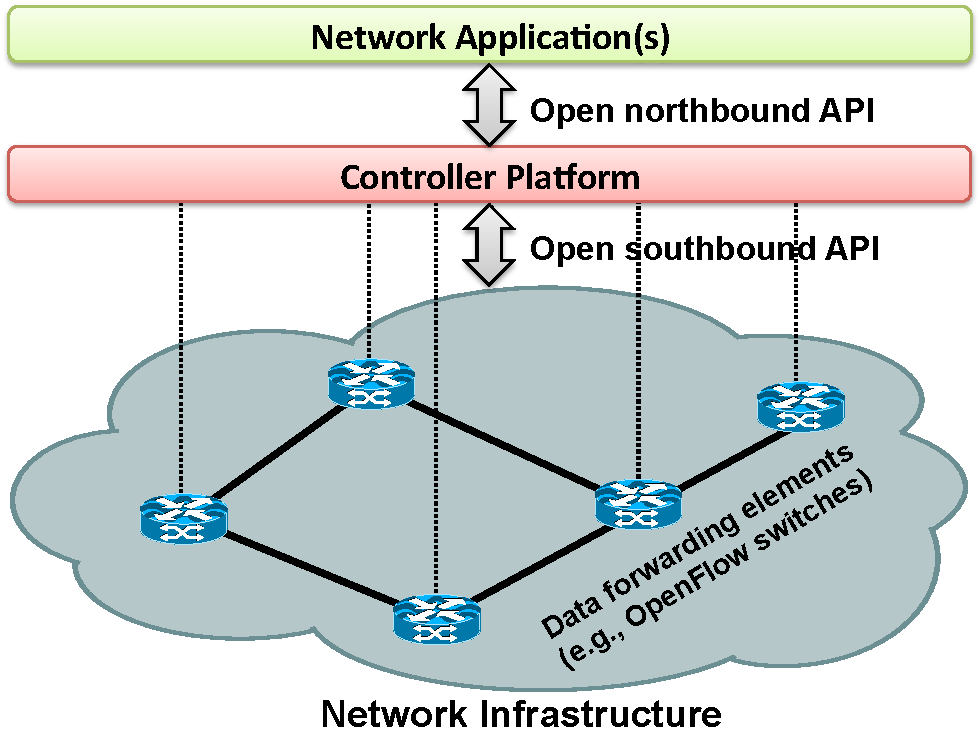
\includegraphics[width=0.95\columnwidth]{figures/fig1_sdn_simple.pdf}
\caption{Simplified view of an SDN architecture.}
\label{fig:sdn_simple}
\end{figure}

% Openflow as enabler
The separation of the control plane and the data plane can be realized
by means of a well-defined programming interface between the switches
and the SDN controller.  The controller exercises direct control over
the state in the data-plane elements via this well-defined application programming interface (API), as
depicted in Figure~\ref{fig:sdn_simple}.  The most notable example of
such an API is OpenFlow~\cite{mckeown2008, onf2013-3}.  An OpenFlow
switch has one or more tables of packet-handling rules (flow table).  
Each rule matches a subset of the traffic and performs certain actions (dropping,
forwarding, modifying, etc.) on the traffic.
%, matching the rule, which matches the rule.
Depending on the rules installed by a controller application, an
OpenFlow switch can -- instructed by the controller -- behave like a
router, switch, firewall, or perform other roles (e.g., load balancer, traffic shaper, and in general those of a
middlebox).

% SDN allows new abstractions and network evolution
An important consequence of the software-defined networking principles
is the \textit{separation of concerns} introduced between the
\textit{definition} of network policies, their \textit{implementation}
in switching hardware, and the \textit{forwarding} of traffic. This separation is key to the
desired flexibility, breaking the network control problem into
tractable pieces, and making it easier to create and introduce new
abstractions in networking, simplifying network management and
facilitating network evolution and innovation.

%SDN - current status
Although SDN and OpenFlow started as academic
experiments~\cite{mckeown2008}, they gained significant traction in the
industry over the past few years.  Most vendors of commercial switches
now include support of the OpenFlow API in their equipment. The SDN momentum 
was strong enough to make Google, Facebook, Yahoo, Microsoft, Verizon, and Deutsche Telekom fund Open Networking Foundation~(ONF)~\cite{onf2013-3} with the main
goal of promotion and adoption of SDN through open standards development. %driven by the users (i.e., equipment buyers) rather than the vendors (i.e., equipment manufacturers). 
  As the initial concerns with SDN scalability were addressed~\cite{yeganeh2013}
-- in particular the myth that logical centralization implied a
physically centralized controller, an issue we will return to later on
-- SDN ideas have matured and evolved from an academic exercise to
a commercial success. Google, for example, has deployed a software-defined
network to interconnect its data centers across the globe. This production 
network has been in deployment for 3 years, helping the company to improve 
operational efficiency and significantly reduce costs~\cite{jain2013-1}.
VMware's network virtualization platform, NSX~\cite{vmware2013},
is another example.  NSX is a commercial solution that delivers a
fully functional network in software, provisioned independent of the
underlying networking devices, entirely based around SDN principles.  As
a final example, the world's largest IT companies (from carriers and
equipment manufacturers to cloud providers and financial-services
companies) have recently joined SDN consortia such as the ONF  and the OpenDaylight initiative~\cite{opendaylight2013}, 
another indication of the importance of SDN from an industrial perspective.

\coloredtext{A few recent papers have surveyed specific architectural aspects of SDN~\cite{lara2014,nunes2014,jarraya2014}.
An overview of OpenFlow and a short literature review can be found in~\cite{lara2014} and~\cite{nunes2014}.
These OpenFlow-oriented surveys present a relatively simplified three-layer stack composed of high-level network services, controllers, and the controller/switch interface.
In~\cite{jarraya2014}, the authors go a step further by proposing a taxonomy for SDN.
However, similarly to the previous works, the survey is limited in terms of scope and it does not provide an in-depth treatment of fundamental aspects of SDN. 
In essence, existing surveys lack a thorough discussion of the essential building blocks of an SDN such as the network operating systems, programming languages, and interfaces.
They also fall short on the analysis of cross-layer issues such as scalability, security, and dependability.
A more complete overview of ongoing research efforts, challenges, and related standardization activities  is also missing.}


\begin{figure*}[t]
\centering
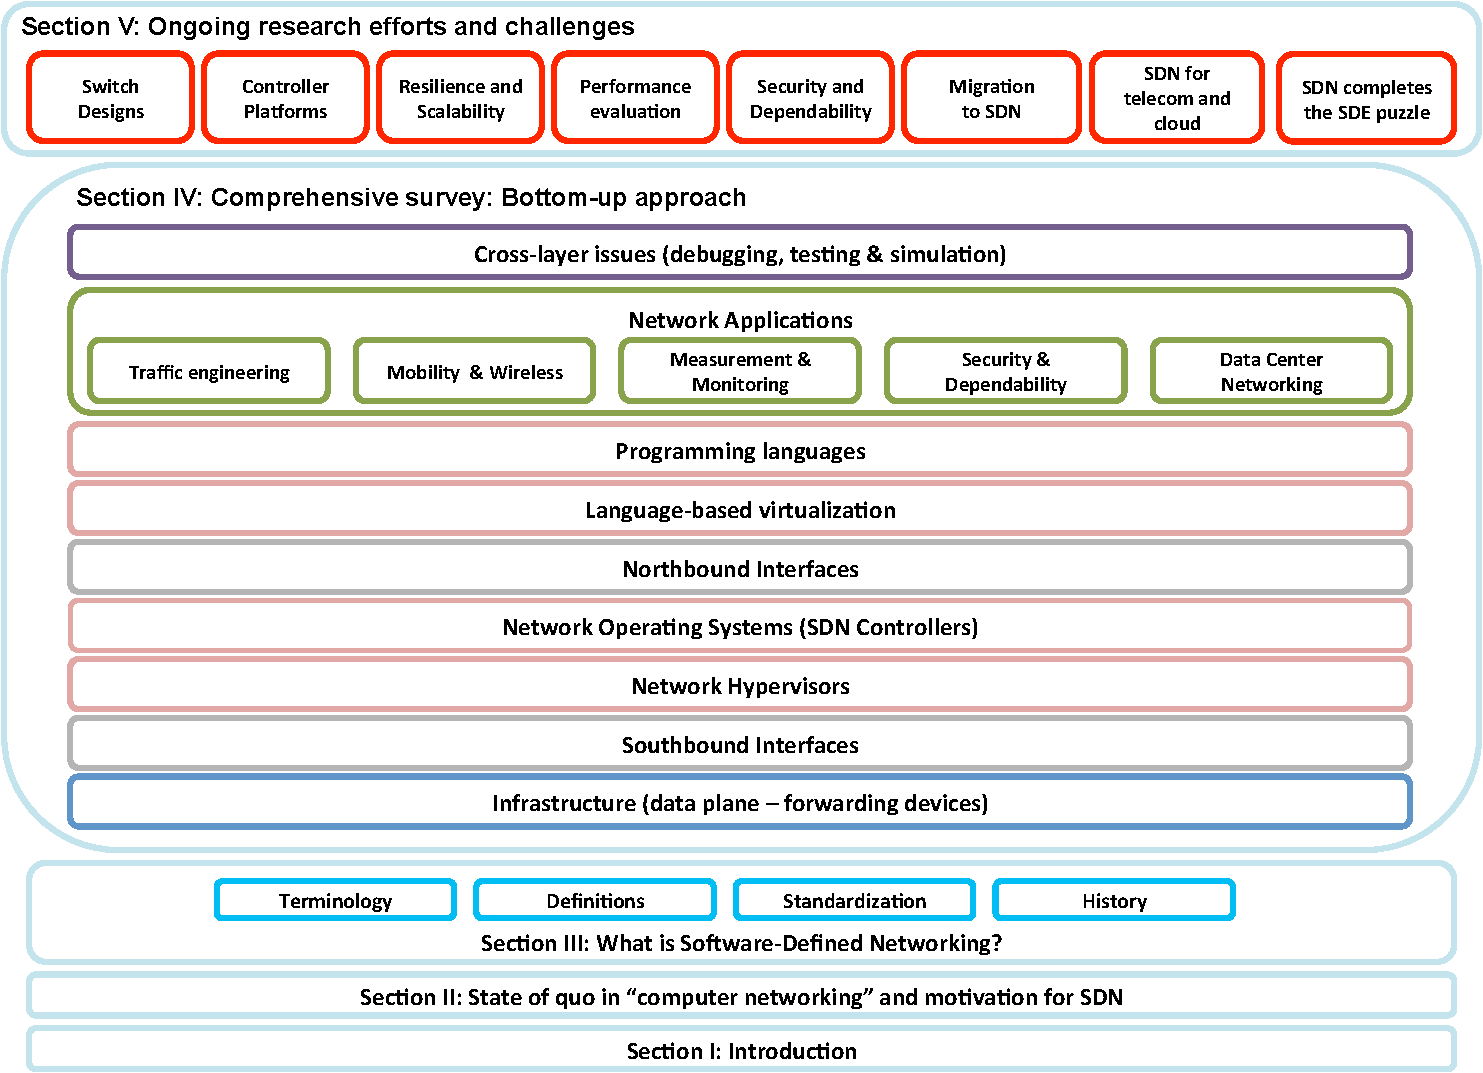
\includegraphics[width=0.95\textwidth]{figures/fig12_survey_condensed_overview.pdf}
\caption{Condensed overview of this survey on SDN.}
\label{fig:conclusion}
\end{figure*}


%This paper
\coloredtext{In this paper, we present, to the best of our knowledge, the most comprehensive literature survey on SDN to date.
We organize this survey} as depicted in Figure~\ref{fig:conclusion}.  We start, in the next two sections, by explaining the context,
introducing the motivation for SDN and explaining the main concepts
of this new paradigm and how it differs from traditional networking.
Our aim in the early part of the survey is also to explain that SDN 
is not as novel as a technological advance.  Indeed, its existence 
is rooted at the intersection of a series of ``old'' ideas, 
technology drivers, and current and future needs. The concepts underlying SDN -- the 
separation of the control and data planes, the  flow abstraction upon
which forwarding decisions are made, the (logical) centralization of
network control, and the ability 
to program the network -- are not novel by themselves~\cite{feamster2013-2}.
However, the integration of already tested concepts with recent trends 
in networking -- namely the availability of merchant switch silicon and
the huge interest in feasible forms of network virtualization -- are
leading to this paradigm shift in networking. 
\coloredtext{As a result of the high industry interest and the potential to 
change the status quo of networking from multiple perspectives, a number of standardization efforts around SDN are ongoing, as we also discuss in Section~\ref{fig:sec-sdn-what}.}

\coloredtext{Section~\ref{sec:layeredapproach} is the core of this}
survey, presenting an extensive and comprehensive
analysis of the building blocks of an SDN infrastructure using a
bottom-up, layered approach.  The option for a layered approach is
grounded on the fact that SDN allows thinking of networking along two
fundamental concepts, which are common in other disciplines of 
computer science: a) separation of concerns (leveraging the concept of abstraction) and b) recursion.
Our layered, bottom-up approach divides the networking problem into eight parts: 1) hardware infrastructure, 2) southbound interfaces, 3) network virtualization (hypervisor layer between 
the forwarding devices and the network operating systems), 4) network operating 
systems (SDN controllers and control platforms), 5) northbound interfaces 
(to offer a common programming abstraction to the upper layers, mainly the network applications), 6) virtualization using slicing techniques provided by special purpose 
libraries or programming languages and compilers, 7) network 
programming languages, and finally 8) network applications. In addition, 
we also look at cross-layer problems such as debugging and troubleshooting 
mechanisms. The discussion in Section~\ref{sec:challenges} on ongoing research efforts, challenges, future work and opportunities concludes this paper.


%\section{Traditional IP Networks}
\section{State of Quo in Networking}
\label{traditional_nets}

Computer networks can be divided in three planes of functionality: the
data, control and management planes (see Figure~\ref{fig:currentnetplanes}).  
The data plane corresponds to the networking devices, which are responsible 
for (efficiently) forwarding data.  The control plane represents the protocols 
used to populate the forwarding tables of the data plane elements. The management 
plane includes the software services, such as SNMP-based tools~\cite{presuhn2002}, 
used to remotely monitor and configure the control functionality.  Network policy 
is defined in the management plane, the control plane enforces the policy, and the 
data plane executes it by forwarding data accordingly.

\begin{figure}[t!]
\centering
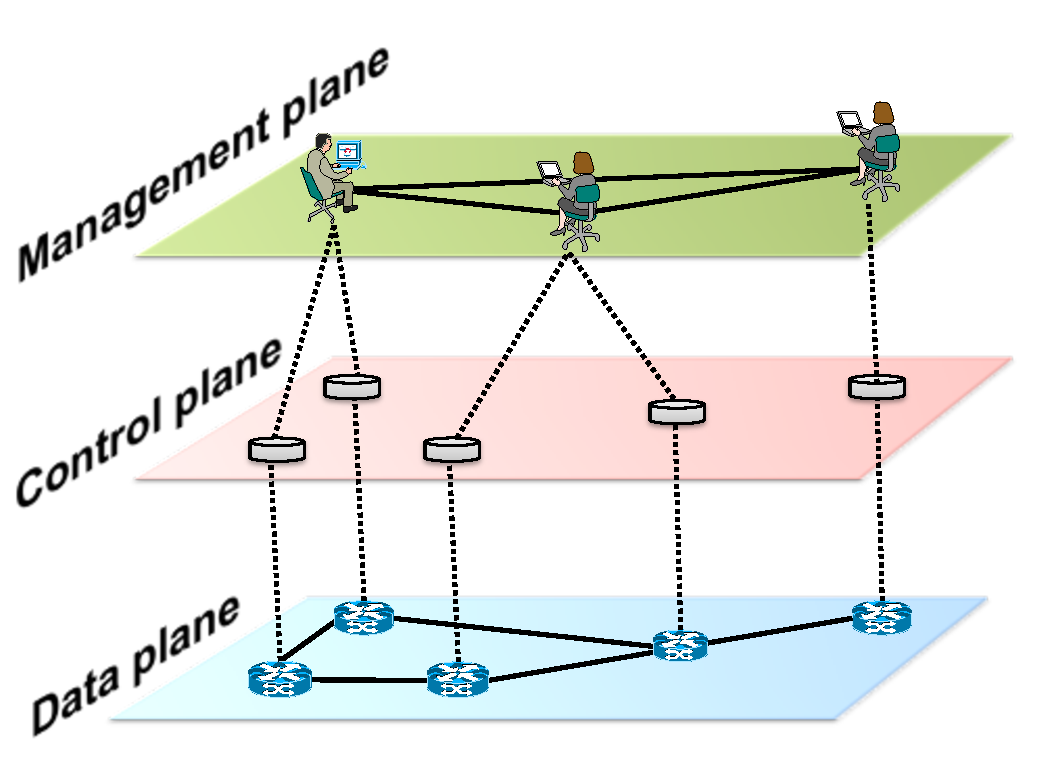
\includegraphics[width=0.75\columnwidth]{figures/fig2_network_functionality.pdf}
\caption{Layered view of networking functionality.}
\label{fig:currentnetplanes}
\end{figure}

In traditional IP networks, the control and data planes are tightly coupled, and 
embedded in the same networking devices, and the whole structure is highly decentralized.
This was considered important for the design of the Internet in the early days: it seemed 
the best way to guarantee network resilience, which was a crucial design goal. In fact, 
this approach has been quite effective in terms of network performance, with a rapid 
increase of line rate and port densities.

However, the outcome is a very complex and relatively static architecture. It is also the 
fundamental reason why traditional networks are rigid, and complex to manage and control.
These two characteristics are largely responsible for a vertically-integrated industry where 
innovation is difficult.

Network misconfigurations and related errors are extremely common in today's networks. 
For instance, more than 1000 configuration errors have been observed in BGP 
routers~\cite{feamster2005}. A single misconfigured device can be a big 
headache for network operators and may have extremely severe consequences. Indeed, while
rare, a single misconfigured router is able to compromise the correct operation of the 
whole Internet for hours~\cite{barrett1997,butler2010}. 

To support network management, a small number of vendors offer proprietary solutions of 
specialized hardware, operating systems, and control programs (network applications). 
Network operators have to acquire and maintain different management solutions and the 
corresponding specialized teams.  The capital and operational cost of building and 
maintaining a networking infrastructure is significant, with long return on investment 
cycles, which hamper innovation and addition of new features and services (for instance 
access control, load balancing, energy efficiency, traffic engineering).  
To alleviate the lack of in-path functionalities within the network, a myriad of specialized 
components and middleboxes, such as firewalls, intrusion detection systems and deep packet inspection engines, proliferate 
in current networks. A recent survey of 57 enterprise networks shows that the number of 
middleboxes is already on par with the number of routers in current networks~\cite{sherry2012}.
Despite helping in-path functionalities, the net effect of middleboxes has been increased
complexity of network design and its operation.

% EOF: 1_traditionl_nets.tex

\section{What is Software-Defined Networking?}
\label{fig:sec-sdn-what}

The term SDN (Software-Defined Networking)  was originally coined to represent 
the ideas and work around OpenFlow at Stanford University~\cite{greene2009}. 
As originally defined, SDN refers to a network architecture where the forwarding 
state in the data plane is managed by a remote control plane decoupled from the former.
The networking industry has on many occasions shifted from this original view of SDN, 
by referring to anything that involves software as being SDN. 
%\coloredtext{One of the main reasons behind this confusing 'noise' around SDN is that every player has something to gain or to lose, so vested interests cannot be ignored~\cite{Reinecke2014}.} 
We therefore attempt, in this section, to provide a much less ambiguous definition of software-defined 
networking.

%SDN: key characteristics.
We define an SDN as a network archi\-te\-cture with four pillars:\\
\begin{enumerate}
\item  The control and data planes are \textit{decoupled}. Control functionality is 
removed from network devices that will become simple (packet) forwarding elements.
\item  Forwarding decisions are flow-based, instead of des\-ti\-na\-tion-based. A flow is 
broadly defined by a set of packet field values acting as a match (filter) criterion 
and a set of actions (instructions).
\coloredtext{In the SDN/OpenFlow context, a flow is a sequence of packets between a source and a destination.
All packets of a flow receive identical service policies at the forwarding devices~\cite{newman1998IP,gude2008}.}
%In other words, once control has been applied on one packet, all following packets with the same header are handled in the same way~\cite{gude2008}.}
The flow abstraction allows unifying the behavior of 
different types of network devices, including routers, switches, firewalls, and \coloredtext{middleboxes~\cite{Jamjoom2014_4}}. 
Flow programming enables unprecedented flexibility, limited only to the capabilities of 
the implemented flow tables~\cite{mckeown2008}. 
%\coloredtext{For instance, firewalls and middleboxes can become middlepipes~\cite{Jamjoom2014_4} and dynamically move, as logical entities opposed to physical devices, to where the services are.}
\item Control logic is moved to an external entity, the so-called SDN controller or Network 
Operating System (NOS). The NOS is a software platform that runs on commodity server technology 
and provides the essential resources and abstractions to facilitate the programming of forwarding 
devices based on a logically centralized, abstract network view. Its purpose is therefore similar 
to that of a traditional operating system.
\item The network is \textit{programmable} through software applications running on top of the NOS that 
interacts with the underlying data plane devices. This is a fundamental characteristic of SDN, considered 
as its main value proposition.
\end{enumerate}

Note that the logical centralization of the control logic, in particular, offers several 
additional benefits.  First, it is simpler and less error-prone to modify network policies 
through high-level languages and software components, compared with low-level device specific
configurations. Second, a control program can automatically react to spurious changes of the 
network state and thus maintain the high-level policies intact. Third, the centralization of 
the control logic in a controller with global knowledge of the network state simplifies the
development of more sophisticated networking functions, services and applications.

Following the SDN concept introduced in~\cite{schenker2011}, an SDN can be defined by 
three fundamental abstractions: (\textit{i}) forwarding, (\textit{ii}) distribution, and 
(\textit{iii}) specification.
In fact, abstractions are essential tools of research in computer science and information technology, being already an ubiquitous feature of many computer architectures and systems~\cite{alkhatib2014}.


Ideally, the \textit{forwarding abstraction} should allow any forwarding behavior desired 
by the network application (the control program) while hiding details of the underlying hardware.
\coloredtext{OpenFlow is one realization of such abstraction}, which can be seen as the equivalent 
to a ``device driver'' in an operating system.

The \textit{distribution abstraction} should shield SDN applications from the vagaries 
of distributed state, making the distributed control problem a logically centralized one.  Its
realization requires a common distribution layer, which in SDN resides in the NOS. This layer has 
two essential functions. First, it is responsible for installing the control commands on the 
forwarding devices.  Second, it collects status information about the forwarding layer (network 
devices and links), to offer a global network view to network applications.

The last abstraction is \textit{specification}, which should allow a network application to express 
the desired network behavior without being responsible for implementing that behavior itself.
This can be achieved through virtualization solutions, as well as network programming languages.
These approaches map the abstract configurations that the applications express based on a simplified, 
abstract model of the network, into a physical configuration for the global network view exposed by 
the SDN controller. Figure~\ref{fig:sdn_abstractions} depicts the SDN architecture, concepts and 
building blocks.
%illustrates these ideas pictorially.
% Note: maybe, it could be a good idea to give a more practical example for "specification abstractions". Maybe something related with the last paper of Jen (USENIX Login). Example: an abstraction could be a view of the network as a single big switch, mapped on a set of physical devices (e.g. four switches).

\begin{figure}[t!]
\centering
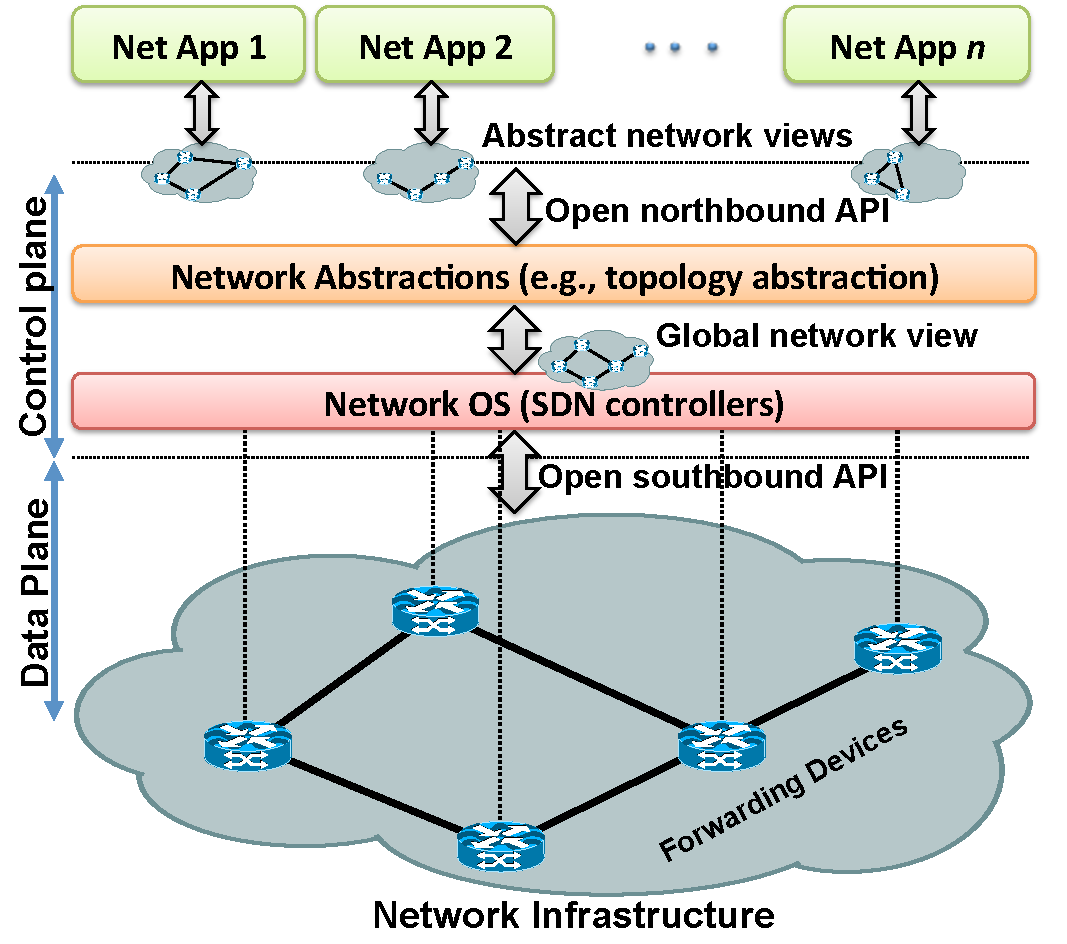
\includegraphics[width=0.95\columnwidth]{figures/fig3_sdn_abstractions.pdf}
\caption{SDN architecture and its fundamental abstractions.}
\label{fig:sdn_abstractions}
\end{figure}

As previously mentioned, the strong coupling between control and data planes has made it difficult 
to add new functionality to traditional networks, \coloredtext{
a fact illustrated in Figure~\ref{fig:traditionalversusSDN}.
The coupling of the control and data planes (and its physical embedding in the network elements) makes the development and deployment of new networking features (e.g., routing algorithms) very hard since 
it would imply a modification of the control plane of all network devices -- through the installation of new firmware and, in some cases, hardware upgrades.
Hence, the new networking features are commonly introduced via expensive, specialized and hard-to-configure equipment (aka middleboxes) such as load balancers, intrusion detection systems (IDS), and firewalls, among others.  
%are common examples.
 These middleboxes need to be placed strategically in the network, making it 
even harder to later change the network topology, configuration, and functionality.}
%For instance, an intrusion detection system might need to receive a cloned copy of the traffic of all switching devices of the network through specific physical and or logical links.
%Moreover, these specialized devices have usually to be configured in a standalone or specific way because each of them has its own (most of time proprietary) interface and configuration protocols.
%On the former we have a strong coupling between control and data planes.
%Appliances such as firewalls and load balancers have to be installed in specific physical spots of the network.
%Moreover, forwarding devices are managed separately from other elements of the network, adding diversity and complexity to the network management and operation tasks.

\begin{figure}[t!]
\centering
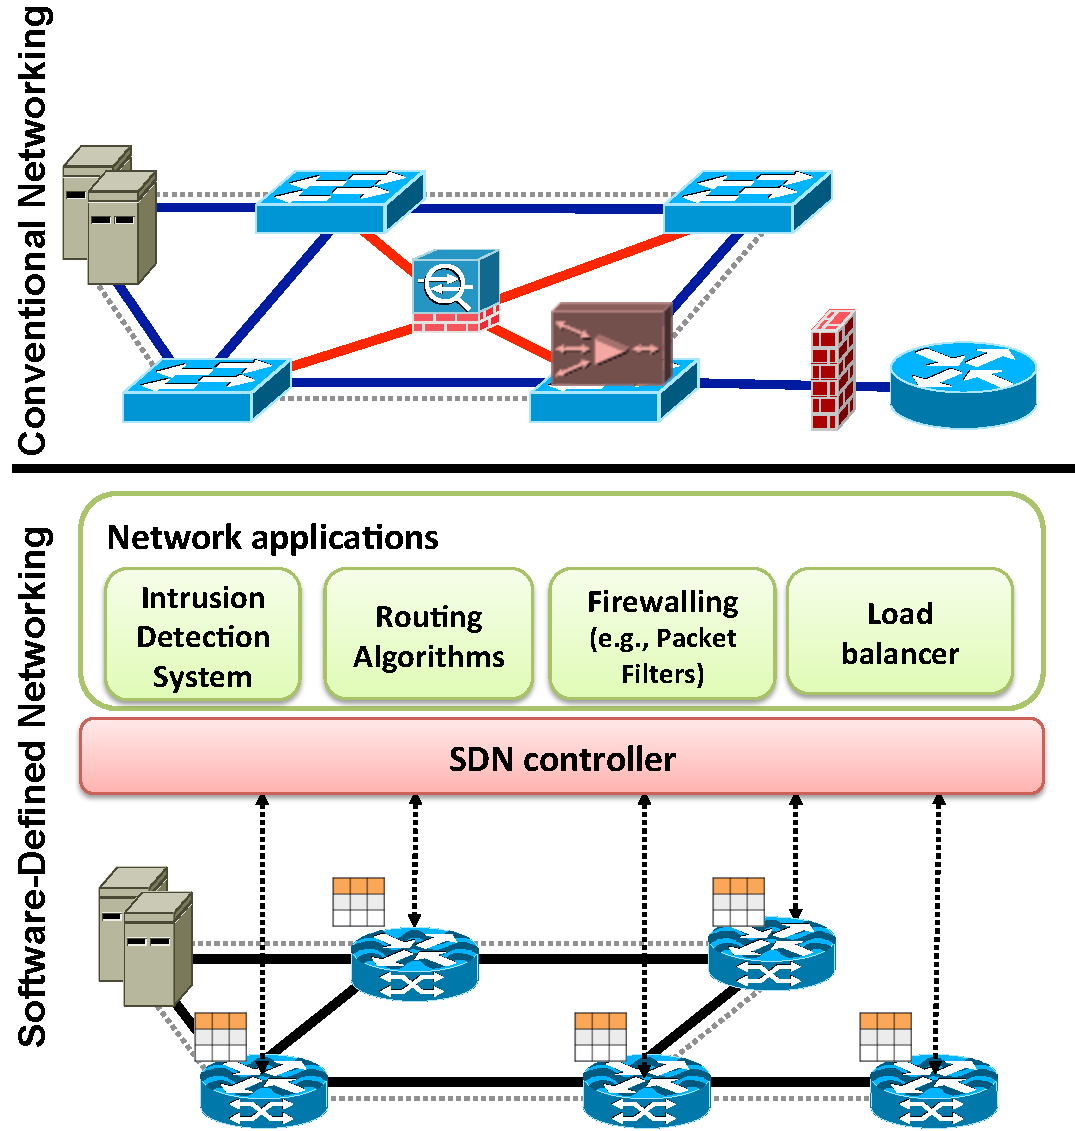
\includegraphics[width=0.95\columnwidth]{figures/fig4_traditional_and_sdn.pdf}
\caption{Traditional networking versus Software-Defined Networking (SDN). With SDN, management becomes simpler and middleboxes services can be delivered as SDN controller applications.}
\label{fig:traditionalversusSDN}
\end{figure}

\coloredtext{In contrast, SDN decouples the control plane from the network devices and becomes an external entity: the network operating system or SDN controller.}
%In other words, the control plane complexity of traditional networks is assembled in a 'single' software-based entity, the controller, which gives move flexibility and speed in terms of changes (e.g., updates and upgrades) and innovation.
%Decoupling devices and programs from the physical topology simplifies applications and allows different programs to co-exist on the same network without interference~\cite{Casado2014_4}.
%Moreover, introducing new functionality in SDN is made simply by adding a new software application to run on top of the NOS.
%For instance, a firewall becomes a simple software application running on top of the NOS and the security policies can be spread across the network devices, i.e., the firewall rules do not need to be applied in a single point or only in a specific device.}
This approach has several advantages:
\begin{itemize}
\item It becomes easier to program these applications since the abstractions provided by the 
control platform and/or the network programming languages can be shared.
\item All applications can take advantage of the same network information (the global network view), 
leading (arguably) to more consistent and effective policy decisions while re-using control plane 
software modules.
\item These applications can take actions (i.e., reconfigure forwarding devices) from any part of 
the network. There is therefore no need to devise a precise strategy about the location of the new 
functionality.
\item The integration of different applications becomes more straightforward~\cite{Casado2014_4}. For instance, load 
balancing and routing applications can be combined sequentially, with load balancing decisions having 
precedence over routing policies.
\end{itemize}
%Essentially, an SDN data plane is comprised of forwarding devices devoid of intelligence.
%Their only task is to process incoming packets based on match and action rules defined by applications running on top of controllers.
%A logically-centralized controller, or network operating system (NOS), abstracts the network for the applications, providing a global view that makes the network look like a single big switch or router.
%The NOS is responsible of dealing with the data collection and distribution to and from data plane devices.
%This data is basically of three types: (1) configuration and forwarding rules sent by the controller to program the device; (2) requests from data plane devices; (3) statistics from the network requested/sent through push or pull interfaces.
%
%In the SDN world OpenFlow is an open standard developed to materialize the clear separation between control and data plane functionalities.
%A controller keeps communication channels with data plane devices, through which it sends and receives OpenFlow messages.
%Forwarding devices can send the first packet of a flow to the controller when they do not know what to do with it.
%These requests are passed up to applications that implement the control logic.
%Their task is to analyze the request, look for policies to be applied and generate rules to be installed on the forwarding elements of the network.

%A data plane device's request can trigger the installation of flow rules in multiple devices.
%For instance, packets of a new flow A should routed to a service B.
%To setup the flow path the controller will have to program all forwarding devices up to service B.
%The forwarding rules are installed in a flow table, used by the device for matching incoming packets and take respective actions (e.g. forward, drop).
%Thereupon, the controller can be seen as  a general purpose network policy enforcement point.
%
%
%Finally, SDN is not a new concept.
%The first initiatives to separate control and data plane date back to the 80s, such as the AT\&T's network control point (NCP)~\cite{sheinbein1982}.
%Similarly, the first programmable data plane devices were introduced still in the 90s (e.g., active networks~\cite{tennenhouse1997}).
%
%\note{CH: May be include a discussion on what is NOT SDN. Introduce the SDN taxonomy by Srini here and/or defer the discussion to the Section on History of SDN?}
%\note{DK: Yes, that could be interesting. I think it fits better in the history section.}

%\coloredtext{It is also worth mentioning that the development and evolution of SDN is bringing into the arena new programming models and abstractions for network-wide structures, distributed updates, modular composition, virtualization, formal verification~\cite{Casado2014_4}.
%In fact, a variety of abstractions, in different levels, will be required to fruitfully build the future network operating systems, similarly to what happened with traditional operating systems.
%}

\subsection{Terminology}

To identify the different elements of an SDN as unequivocally as possible, we now present the 
essential terminology used throughout this work.

\noindent \textit{Forwarding Devices (FD)}: Hardware- or software-based data plane devices that perform 
a set of elementary operations. The forwarding devices have well-defined instruction sets (e.g., flow 
rules) used to take actions on the incoming packets (e.g., forward to specific ports, drop, forward to 
the controller, rewrite some header). These instructions are defined by southbound interfaces (e.g., 
OpenFlow~\cite{mckeown2008}, ForCES~\cite{doria2010}, Protocol- Oblivious Forwarding (POF)~\cite{song2013}) and are installed in the forwarding devices by the SDN controllers implementing the southbound protocols.

\noindent \textit{Data Plane (DP)}: Forwarding devices are interconnected through wireless radio channels 
or wired cables. The network infrastructure comprises the interconnected forwarding devices, which 
represent the data plane.
%More specifically, the data plane is the part of the forwarding device which is responsible for receiving and sending packets across the data plane.

\noindent \textit{Southbound Interface (SI)}: The instruction set of the forwarding devices is defined 
by the southbound API, which is part of the southbound interface. Furthermore, the SI also defines the 
communication protocol between forwarding devices and control plane elements. This protocol formalizes 
the way the control and data plane elements interact.

\noindent \textit{Control Plane (CP)}: Forwarding devices are programmed by control plane elements 
through well-defined SI embodiments. The control plane can therefore be seen as the ``network brain''.
All control logic rests in the applications and controllers, which form the control plane.
%At the lowest layer of the control plane, there are southbound interfaces for sending and receiving requests from and to forwarding devices.
%These requests can contain flow control rules to be installed on forwarding devices, or action requests and statistics sent by forwarding devices to control plane elements, such as network operating systems.

\noindent \textit{Northbound Interface (NI)}: The network operating system can offer an API to application 
developers. This API represents a northbound interface, i.e., a common interface for developing applications.
%and interacting with external system such as cloud orchestration services.
Typically, a northbound interface abstracts the low level instruction sets used by southbound interfaces 
to program forwarding devices.

\noindent \textit{Management Plane (MP)}: The management plane is the set of applications that leverage 
the functions offered by the NI to implement network control and operation logic.
This includes applications such as routing, firewalls, load balancers, monitoring, and so forth.
%In other words, the MP accommodates management applications which are responsible for programming, configuring and monitoring the network operation.
Essentially, a management application defines the policies, which are ultimately translated to 
southbound-specific instructions that program the behavior of the forwarding devices.

\subsection{Alternative and Broadening Definitions}
\label{sec:alt-SDN}


Since its inception in 2010~\cite{greene2009}, the original OpenFlow-centered SDN term 
has seen its scope broadened beyond architectures with a cleanly decoupled control plane 
interface. The definition of SDN will likely continue to broaden, driven by the industry 
business-oriented views on SDN -- irrespective of the decoupling of the control plane. In 
this survey, we focus on the original, ``canonical'' SDN definition based on the aforementioned
key pillars and the concept of layered abstractions. However, for the sake of completeness 
and clarity, we acknowledge alternative SDN definitions~\cite{nadeau2013}, including:

%\begin{itemize}
%\item
\noindent \textit{Control Plane / Broker SDN}: A networking approach that retains existing distributed 
control planes but offers new APIs that allow applications to interact (bidirectionally) with the network. 
An SDN controller --often called orchestration platform-- acts as a broker between the applications and 
the network elements. This approach effectively presents control plane data to the application and allows 
a certain degree of network programmability by means of ``plug-ins'' between the orchestrator function and 
network protocols. This API-driven approach corresponds to a hybrid model of SDN, since it enables the broker 
to manipulate and directly interact with the control planes of devices such as routers and switches. Examples 
of this view on SDN include recent standardization efforts at IETF \coloredtext{(see Section~\ref{sec:standardization})} and the design philosophy behind the OpenDaylight project~\cite{opendaylight2013} that goes beyond the OpenFlow split control mode.

%\item 
\noindent \textit{Overlay SDN}: A networking approach where the (software- or hardware-based) network edge 
is dynamically programmed to manage tunnels between hypervisors and/or network switches, introducing an 
overlay network. In this hybrid networking approach, the distributed control plane providing the underlay 
remains untouched. The centralized control plane provides a logical overlay that utilizes the underlay 
as a transport network. This flavor of SDN follows a proactive model to install the overlay tunnels. The overlay
tunnels usually terminate inside virtual switches within hypervisors or in physical devices acting as gateways 
to the existing network. This approach is very popular in recent data center network virtualization \cite{chowdhury2010}, and are based on a variety of tunneling technologies \coloredtext{(e.g., STT~\cite{davie2014stt}, VXLAN~\cite{mahalingam2013}, NVGRE~\cite{sridharan2013}, LISP~\cite{maino2013lisp,hertoghs2014lisp}, GENEVE~\cite{Gross2014_4})}~\cite{jain2013}.

\coloredtext{Recently, other attempts to define SDN in a layered approach have appeared~\cite{haleplidis2014layers,jarraya2014}.
From a practical perspective and trying to keep backward compatibility with existing network management approaches, one  initiative at IRTF SDNRG~\cite{haleplidis2014layers} proposes a management plane at the same level of the control plane, i.e., it classifies solutions in two categories: control logic (with control plane southbound interfaces) and management logic (with management plane southbound interfaces).
In other words, the management plane can be seen as a control platform that accommodates traditional network management services and protocols, such as SNMP~\cite{presuhn2002}, BGP~\cite{rekhter2006}, PCEP~\cite{vasseur2009}, and NETCONF~\cite{enns2011-1}.
}

In addition the broadening definitions above, the term SDN is often used to define extensible network management planes (e.g., OpenStack~\cite{corradi2014}), \coloredtext{
whitebox / bare-metal switches with open operating systems (e.g., Cumulus Linux),} open-source dataplanes (e.g., Pica8 Xorplus~\cite{shang2014}, Quagga~\cite{jakma2014}), specialized programmable hardware devices (e.g., 
NetFPGA~\cite{netfpga2014}), virtualized software-based appliances \coloredtext{(e.g., Open Platform for Network Functions Virtualization - OPNFV~\cite{opnfv})}, in spite of 
lacking a decoupled control and data plane or common interface along its API. Hybrid SDN models are further discussed in Section~\ref{sec:hybrid}. 


\coloredtext{

\subsection{Standardization Activities}
\label{sec:standardization}

The standardization landscape in SDN (and SDN-related issues) is already wide and is expected to keep evolving over time. 
While some of the activities are being carried out in Standard Development Organizations (SDOs), other related efforts are ongoing at industrial or community consortia (e.g., OpenDaylight, OpenStack, OPNFV), delivering results often considered candidates for \textit{de facto} standards.
These results often come in the form of open source implementations that have become the common strategy towards accelerating SDN and related cloud and networking technologies~\cite{floss-meets-sdn}.
The reason for this fragmentation is due to SDN concepts spanning different areas of IT and networking, both from a network segmentation point of view (from access to core) and from a technology perspective (from optical to wireless).

Table~\ref{tab:standardization} presents a summary of the main SDOs and organizations contributing to the standardization of SDN, as well as the main outcomes produced to date.
 
The Open Networking Foundation (ONF) was conceived as a member-driven organization to promote the adoption of SDN through the development of the OpenFlow protocol as an open standard to communicate control decisions to data plane devices. 
The ONF is structured in several working groups (WGs). Some WGs are focused on either defining extensions to the OpenFlow protocol in general, such as the Extensibility WG, or tailored to specific technological areas. 
Examples of the latter include the Optical Transport (OT) WG, the Wireless and Mobile (W\&M) WG, and the Northbound Interfaces (NBI) WG. Other WGs center their activity in providing new protocol capabilities to enhance the protocol itself, such as the Architecture WG or the Forwarding Abstractions (FA) WG.

%The Internet Engineering Task Force (IETF), arguably the most relevant SDO related to Internet protocols, is structured in eight different areas, each comprised of WGs producing technical documents known as Request For Comment (RFC). %, which usually become the norm followed by the industry for specific topics
Similar to how network programmability ideas have been considered by several Working Groups (WGs) of the Internet Engineering Task Force (IETF) in the past, the present SDN trend is also influencing a number of activities. 
A related body that focuses on research aspects for the evolution of the Internet, the Internet Research Task Force (IRTF), has created the Software Defined Networking Research Group (SDNRG).
This group investigates SDN from various perspectives with the goal of identifying the approaches that can be defined, deployed and used in the near term, as well as identifying future research challenges.
%For the sake of completeness, Table~\ref{tab:standardization} includes outcomes related contributions of these WGs, either in the form of stable RFCs, working group accepted documents or individual submissions for discussion.

%The International Telecommunications Union's Telecommunication sector (ITU-T) is an organism of the United Nations, structured in distinct Study Groups (SG) and in charge of developing international standards, in the form of recommendations.
In the International Telecommunications Union's Telecommunication sector (ITU-T), some Study Groups (SGs) have already started to develop recommendations for SDN, 
%including the SG 11 (Signaling requirements, protocols and test specifications), SG 13  (Future networks including cloud computing, mobile and next-generation networks), SG 15 (Networks, Technologies and Infrastructures for Transport, Access and Home), and SG17 (Security). On top of that, the ITU-T has established 
and a Joint Coordination Activity on SDN (JCA-SDN) has been established to coordinate the SDN standardization work.% on SDN and related technical topics within ITU-T.

The Broadband Forum (BBF) is working on SDN topics through the Service Innovation \& Market Requirements (SIMR) WG. The objective of the BBF is to release recommendations for supporting SDN in multi-service broadband networks, including hybrid environments where only some of the network equipment is SDN-enabled.

The Metro Ethernet Forum (MEF) is approaching SDN with the aim of defining service orchestration with APIs for existing networks. %to accommodate NFV and Network-as-a-Service. %This initiative will be called The Third Network, and has been publicly announced in September 2014.

At the Institute of Electrical and Electronics Engineers (IEEE), the 802 LAN/MAN Standards Committee has recently started some activities to standardize SDN capabilities on access networks based on IEEE 802 infrastructure through the P802.1CF project, for both wired and wireless technologies to embrace new control interfaces.% on top of the IEEE 802 infrastructure. 

The Optical Internetworking Forum (OIF) Carrier WG released a set of requirements for Transport Software-Defined Networking. The initial activities have as main goal to describe the features and functionalities needed to support the deployment of SDN capabilities in carrier transport networks.

The Open Data Center Alliance (ODCA) is an organization working on unifying data center in the migration to cloud computing environments through interoperable solutions. Through the documentation of usage models, specifically one for SDN, the ODCA is defining new requirements for cloud deployment. 

The Alliance for Telecommunication Industry Solutions (ATIS) created a Focus Group for analyzing operational issues and opportunities associated with the programmable capabilities of network infrastructure. %The result of this competed activity was the release of a report covering such analysis.

At the European Telecommunication Standards Institute (ETSI), efforts are being devoted to Network Function Virtualization (NFV) through a newly defined Industry Specification Group (ISG). 
NFV and SDN concepts are considered complementary, sharing the goal of accelerating innovation inside the network by allowing programmability, and altogether changing the network operational model through automation and a real shift to software-based platforms.
%Architectural work at ETSI NFV ISG defines the presence of orchestration capabilities including computing, storage and networking, tightly linked to SDN concepts.

Finally, the mobile networking industry 3GPP consortium is studying the management of virtualized networks, an effort aligned with the ETSI NFV architecture and, as such, likely to leverage from SDN.

{\renewcommand{\arraystretch}{1.4}
\begin{table*}[!htp]
\caption{\coloredtext{OpenFlow standardization activities}}
\label{tab:standardization}
\begin{center}
\footnotesize
%\rowcolors{1}{lightgray}{white}
%\rowcolors{1}{red!45}{red!45}
\begin{tabularx}{\linewidth}{p{0.8cm}p{3.8cm}Xp{4.6cm}}
\hline
%\rowstyle{\color{red}}
%\colorrows{\color{red}}
\textbf{SDO} & \textbf{Working Group} & \textbf{Focus}  & \textbf{Outcomes} \\
\hline
%\rowstyle{\color{red}}
\multirow{16}{*}{ONF} 
& Architecture \& Framework & SDN architecture, defining architectural components and interfaces & SDN Architecture~\cite{SDNARCH}  \\\cline{2-4}

& Northbound Interfaces & Definition of standard NBIs for SDN controllers	& \\\cline{2-4}

& Testing and Interoperability	& Specification of OpenFlow conformance test suites	& Conformance tests~\cite{CTSOSS} \\\cline{2-4}

& Extensibility	& Development of extensions to OpenFlow protocol, producing specifications of the OpenFlow switch (OF-WIRE) protocol &	OF-WIRE 1.4.0~\cite{OSS} \\\cline{2-4}

& Configuration \& Management	& OAM (operation, administration, and management) capabilities for OF protocol, producing specifications of the OF Configuration and Management (OF-CONFIG) protocol & OF-CONFIG 1.2~\cite{OFCONFIG} \par OpenFlow Notifications Framework~\cite{onf2013-2} \\\cline{2-4}

& Forwarding Abstractions & Development of hardware abstractions and simplification of behavioral descriptions mapping & OpenFlow Table Type Patterns~\cite{OTTP} \\\cline{2-4}

& Optical Transport	& Specification of SDN and control capabilities for optical transport networks by means of OpenFlow & Use cases~\cite{OTUC} \par Requirements~\cite{RATOSDN} \\\cline{2-4}

& Wireless \& Mobile & Specification of SDN and control capabilities for wireless and mobile networks by means of OpenFlow & \\\cline{2-4}

& Migration	& Methods to migrate from conventional networks to SDN-based networks based on OpenFlow & Use cases~\cite{MUCM} \\\cline{2-4}

& Market Education	& Dissemination of ONF initiatives in SDN and OpenFlow by releasing White Papers and Solution Briefs	& SDN White Paper~\cite{SDN_NNN} \\
\hline
\multirow{15}{*}{IETF} 
& Application-Layer Traffic Optimization (ALTO) &  Provides applications with network state information  &    Architectures for the coexistence of SDN and ALTO~\cite{xie2012} \\\cline{2-4}

& Forwarding and Control Element Separation (ForCES) & Protocol specifications for the communication between control and forwarding elements. & Protocol specification~\cite{doria2010} \\\cline{2-4}

& Interface to the Routing System (I2RS) & Real-time or event driven interaction with the routing system in an IP routed network	& Architecture~\cite{AIRS} \\\cline{2-4}

& Network Configuration (NETCONF) & Protocol specification for transferring configuration data to and from a device & NETCONF protocol~\cite{enns2004} \\\cline{2-4}

& Network Virtualization Overlays (NVO3) & Overlay networks for supporting multi-tenancy in the context of data center communications (i.e., VM communication) & Control plane requirements~\cite{NVENVA} \\\cline{2-4}

& Path Computation Element (PCE) & Path computation for traffic engineering and path selection based on constrains & ABNO framework~\cite{PCE} \par Cross stratum path computation~\cite{CSOPC} \\\cline{2-4}

& Source Packet Routing in Networking (SPRING) & Specification of a forwarding path at the source of traffic	 & OpenFlow interworking~\cite{khasnabish2014} \par SDN controlled use cases~\cite{kim2014} \\\cline{2-4}

& Abstraction and Control of Transport Networks (ACTN) BoF & Facilitate a centralized virtual network operation	 &   Virtual network controller framework~\cite{ceccarelli2014} \\
\hline
IRTF & Software-Defined Networking Research Group (SDNRG) & Prospection of SDN for the evolution of Internet & SDN operator perspective~\cite{boucadair2014} \par SDN Architecture~\cite{haleplidis2014} \par
 Service / Transport separation~\cite{contreras2014} \\
 \hline
\multirow{7}{*}{ITU-T} 
& SG 11 & Signalling requirements using SDN technologies in Broadband Access Networks & Q.Supplement-SDN~\cite{itutqsup2014} \par Q.SBAN~\cite{itutqsban2014} \\\cline{2-4}

& SG 13 & Functional requirements and architecture for SDN and networks of the future & Recommendation Y.3300~\cite{ituty33002014} \\\cline{2-4}

& SG 15 & Specification of a transport network control plane architecture to support SDN control of transport networks & \\\cline{2-4}

& SG 17 & Architectural aspects of security in SDN and security services using SDN & \\
\hline
BBF & Service Innovation and Market Requirements & Requirements and impacts of deploying SDN in broadband networks & SD-313~\cite{bforum2014}\\
\hline
MEF & The Third Network & Service orchestration in Network as a Service and NFV environments & \\
\hline
IEEE & 802 & Applicability of SDN to IEEE 802 infrastructure & \\
\hline
OIF & Carrier WG & Transport SDN networks & Requirements for SDN enabled transport networks~\cite{oif2013}\\
\hline
ODCA & SDN/Infrastructure  & Requirements for SDN in cloud environments & Usage model~\cite{odc2014}\\
\hline
ETSI & NFV ISG & Orchestration of network functions, including the combined control of computing, storage and networking resources & NFV Architecture~\cite{etsi2013}\\
\hline
ATIS & SDN Focus Group & Operational aspects of SDN and NFV & Operation of SDN~\cite{atis2014}\\
\hline
\end{tabularx}
\end{center}
\end{table*}
}



} % coloredtext
\subsection{History of Software-Defined Networking}

Albeit a fairly recent concept, SDN leverages on networking ideas with a longer history~\cite{feamster2013-2}.
In particular, it builds on work made on programmable networks, such as active networks~\cite{tennenhouse1997}\coloredtext{, programmable ATM networks~\cite{lazar1996,lazar1997} }, and on proposals for control and data plane separation, such as NCP~\cite{sheinbein1982} and RCP~\cite{caesar2005}.

In order to present an historical perspective, we summarize in Table~\ref{tab:history} different instances of SDN-related work prior to SDN, splitting it into five categories.
Along with the categories we defined, the second and third columns of the table mention past initiatives (pre-SDN, i.e., before the OpenFlow-based initiatives that sprung into the SDN concept), and recent developments that led to the definition of SDN.


\newcommand{\fcwidth}{3.2cm}
\newcommand{\scwidth}{9.2cm}
\newcommand{\tcwidth}{4.6cm}
{\renewcommand{\arraystretch}{1.4}
\begin{table*}[!htp]
\caption{Summarized overview of the history of programable networks}
\label{tab:history}
\begin{center}
\footnotesize
\begin{tabularx}{\linewidth}{p{\fcwidth}p{\scwidth}p{\tcwidth}}
\hline
\textbf{Category} & \textbf{Pre-SDN initiatives} & \textbf{More recent SDN developments} \\
\hline
\multirow{2}{*}{\begin{minipage}{\fcwidth}
		Data plane programmability
	\end{minipage}} 
& \multirow{2}{*}{\begin{minipage}{\scwidth}
		\coloredtext{xbind~\cite{lazar1996},}
		IEEE P1520~\cite{biswas1998},
		smart packets~\cite{schwartz1999},
		ANTS~\cite{wetherall1998},
		SwitchWare~\cite{alexander1998},
		Calvert~\cite{calvert1998},
		high performance router~\cite{wolf2000},
		NetScript~\cite{silva2001},
		Tennenhouse~\cite{tennenhouse2007}
	\end{minipage}} 
& \multirow{2}{*}{
	\begin{minipage}{\tcwidth}
		ForCES~\cite{doria2010},
		OpenFlow~\cite{mckeown2008},
		POF~\cite{song2013}
	\end{minipage}} \\
& & \\
\hline
\multirow{2}{*}{\begin{minipage}{\fcwidth}
		Control and data plane \\decoupling
	\end{minipage}} 
& \multirow{2}{*}{\begin{minipage}{\scwidth}
		NCP~\cite{sheinbein1982},
		\coloredtext{GSMP~\cite{rfc1987,rfc3294}},
		Tempest~\cite{merwe1998},
		%Click~\cite{morris1999},
		ForCES~\cite{doria2010},
		RCP~\cite{caesar2005},
		SoftRouter~\cite{lakshman2004},
		PCE~\cite{vasseur2009},
		4D~\cite{greenberg2005},
		IRSCP~\cite{merwe2006}
	\end{minipage}} 
& \multirow{2}{*}{
	\begin{minipage}{\tcwidth}
		SANE~\cite{casado2006},
		Ethane~\cite{casado2007-1},
		OpenFlow~\cite{mckeown2008},
		NOX~\cite{gude2008},
		POF~\cite{song2013}
	\end{minipage}} \\
& & \\
\hline
\multirow{2}{*}{\begin{minipage}{\fcwidth}
		Network virtualization
	\end{minipage}} 
& \multirow{2}{*}{\begin{minipage}{\scwidth}
		Tempest~\cite{merwe1998},
		MBone~\cite{macedonia1994},
		6Bone~\cite{fink2004},
		RON~\cite{andersen2001},
		Planet Lab~\cite{chun2003},
		Impasse~\cite{anderson2005},
		GENI~\cite{peterson2006},
		VINI~\cite{bavier2006-1}
	\end{minipage}} 
& \multirow{2}{*}{
	\begin{minipage}{\tcwidth}
		Open vSwitch~\cite{pfaff2009},
		Mininet~\cite{lantz2010},
		FlowVisor~\cite{sherwood2010},
		NVP~\cite{koponen}
	\end{minipage}} \\
& & \\
\hline
\multirow{1}{*}{\begin{minipage}{\fcwidth}
		Network operating systems
	\end{minipage}} 
& \multirow{1}{*}{\begin{minipage}{\scwidth}
		Cisco IOS~\cite{bollapragada2000},
		JUNOS~\cite{junipernetworks2012}.
		ExtremeXOS~\cite{extremenetworks2014},
		SR OS~\cite{alcatellucent2014}
	\end{minipage}} 
& \multirow{1}{*}{
	\begin{minipage}{\tcwidth}
		NOX~\cite{gude2008},
		Onix~\cite{koponen-1},
		ONOS~\cite{krishnaswamy2013}
	\end{minipage}} \\
\hline
\multirow{1}{*}{\begin{minipage}{\fcwidth}
		Technology pull initiatives
	\end{minipage}} 
& \multirow{1}{*}{\begin{minipage}{\scwidth}
	Open Signaling~\cite{campbell1999}
	\end{minipage}} 
& \multirow{1}{*}{
	\begin{minipage}{\tcwidth}
	ONF~\cite{onf2013-3}
	\end{minipage}} \\
\hline
\end{tabularx}
\end{center}
\end{table*}
}

Data plane programmability has a long history. Active networks~\cite{tennenhouse1997} 
represent one of the early attempts on building new network architectures based on this concept.
The main idea behind active networks is for each node to have the capability to perform computations 
on, or modify the content of, packets. To this end, active networks propose two distinct approaches: 
programmable switches and capsules. The former does not imply changes in the existing packet or cell 
format. It assumes that switching devices support the downloading of programs with specific instructions 
on how to process packets. The second approach, on the other hand, suggests that packets should be 
replaced by tiny programs, which are encapsulated in transmission frames and executed at each node 
along their path.

ForCES~\cite{doria2010}, OpenFlow~\cite{mckeown2008} and POF~\cite{song2013}  represent recent approaches for designing and deploying programmable data plane devices.
In a manner different from active networks, these new proposals rely essentially on modifying forwarding devices to support flow tables, which can be dynamically configured by remote entities through simple operations such as adding, removing or updating flow rules, i.e., entries on the flow tables.

The earliest initiatives on separating data and control signalling date back to the 80s and 90s.
The network control point (NCP)~\cite{sheinbein1982} is probably the first attempt to separate 
control and data plane signalling. NCPs were introduced by AT\&T to improve the management and control 
of its telephone network. This change promoted a faster pace of innovation of the network and provided 
new means for improving its efficiency, by taking advantage of the global view of the network provided 
by NCPs. Similarly, other initiatives such as Tempest~\cite{merwe1998}, ForCES~\cite{doria2010},
RCP~\cite{caesar2005}, and PCE~\cite{vasseur2009} proposed the separation of the control 
and data planes for improved management in ATM, Ethernet, BGP, and MPLS networks, respectively.

More recently, initiatives such as SANE~\cite{casado2006}, Ethane~\cite{casado2007-1},
OpenFlow~\cite{mckeown2008}, NOX~\cite{gude2008} and POF~\cite{song2013} proposed the decoupling of the control and data planes 
for Ethernet networks. Interestingly, these recent solutions do not require significant modifications 
on the forwarding devices, making them attractive not only for the networking research community, but 
even more to the networking industry. OpenFlow-based devices~\cite{mckeown2008}, 
for instance, can easily co-exist with traditional Ethernet devices, enabling a progressive adoption 
(i.e., not requiring a disruptive change to existing networks).

Network virtualization has gained a new traction with the advent of SDN. Nevertheless, network virtualization 
also has its roots back in the 90s. The Tempest project~\cite{merwe1998} is one of the first initiatives to 
introduce network virtualization, by introducing the concept of switchlets in ATM networks. The core idea 
was to allow multiple switchlets on top of a single ATM switch, enabling multiple independent ATM networks 
to share the same physical resources. Similarly, MBone~\cite{macedonia1994} was one of the early initiatives that 
targeted the creation of virtual network topologies on top of legacy networks, or overlay networks. This work 
was followed by several other projects such as Planet Lab~\cite{chun2003}, GENI~\cite{peterson2006} 
and VINI~\cite{bavier2006-1}. It is also worth mentioning FlowVisor~\cite{sherwood} as one of the first recent initiatives to promote a 
hypervisor-like virtualization architecture for network infrastructures, resembling the hypervisor model 
common for compute and storage.
More recently, Koponen et al. proposed a Network Virtualization Platform (NVP~\cite{koponen}) for multi-tenant datacenters using SDN as a base technology.

The concept of a network operating system was reborn with the introduction of OpenFlow-based network 
operating systems, such as NOX~\cite{gude2008}, Onix~\cite{koponen-1} 
and ONOS~\cite{krishnaswamy2013}. Indeed, network operating systems have been in existence for decades.
One of the most widely known and deployed is the Cisco IOS~\cite{bollapragada2000}, which was originally 
conceived back in the early 90s. Other network operating systems worth mentioning are JUNOS~\cite{junipernetworks2012},
ExtremeXOS~\cite{extremenetworks2014} and SR OS~\cite{alcatellucent2014}. Despite being more specialized 
network operating systems, targeting network devices such as high-performance core routers, these NOSs abstract 
the underlying hardware to the network operator, making it easier to control the network infrastructure as well 
as simplifying the development and deployment of new protocols and management applications.

Finally, it is also worth recalling initiatives that can be seen as ``technology pull'' drivers.
Back in the 90s, a movement towards open signalling~\cite{campbell1999} started 
to happen. The main motivation was to promote the wider adoption of the ideas proposed by projects 
such as NCP~\cite{sheinbein1982} and Tempest~\cite{merwe1998}. The open signalling movement worked 
towards separating the control and data signalling, by proposing open and programmable interfaces.
Curiously, a rather similar movement can be observed with the recent advent of OpenFlow and SDN, with 
the lead of the Open Networking Foundation (ONF)~\cite{onf2013-3}. This type of movement is crucial 
to promote open technologies into the market, hopefully leading equipment manufacturers to support 
open standards and thus fostering interoperability, competition, and innovation.

For a more extensive intellectual history of programmable networks and SDN we forward the reader to 
the recent paper by Feamster et al.~\cite{feamster2013-2}.

%\subsection*{Separating control and data signaling}
%
%Network control point (NCP)~\cite{sheinbein1982} is the first attempt to separate control and data plane signaling.
%NCPs were introduced to improve the management view and control over the AT\&T telephony network.
%This change intrinsically promoted a faster pace of innovation and provided new means to advance the resources utilization efficiency through a global view of the network that was available at the NCPs.
%A global view of the network helps to foster the development of better monitoring and call routing solutions, as was the case of AT\&T, for instance.
%
%One decade later, on the 90s, a movement towards open signaling~\cite{campbell1999} started to happen.
%The core motivation was to remove the network control capabilities from the data plane, i.e., separate control and data signaling through open and programmable interfaces.
%
%The idea of the open signaling movement was to explore avenues to use open and programmable interfaces to have access and manage network hardware.
%This would allow the development and deployment of new services in a more flexible and interoperable way.
%Hence, it can be seen as the next step after the advent of network control points.
%Curiously, a similar movement can be observed with the arriving of SDNs, the open networking, which is leaded by the Open Networking Foundation (ONF)~\cite{onf2013-3}.
%This kind of movement is important to promote open technologies into the market, lead equipment manufacturers to support open standards, foster interoperability, competition, and innovation.
%

%\subsection*{Programmable data plane}
%
%Active networks~\cite{tennenhouse1997} represent one of the early attempts to build new network architectures.
%An active network node can perform computations on or modify the content of packets.
%Additionally, computations can be defined and executed in a per user or per application basis.
%
%Two distinct approaches for active networks were proposed.
%First, programmable switches that do not change the existing packet or cell format.
%These devices should support the downloading of programs with specific instructions on how to process packets.
%The second approach is based on the concept of a capsule.
%It suggests that packets are replaced by tiny programs, which are encapsulated in transmission frames and executed at each node along their path.
%
%%Both programmable switches and capsules were proposed to develop the same key idea: add programmability to the network for customized services.
%%While the former proposes separating the data transfer and management channels, the latter copes with the idea of inserting program fragments in the messages, which are interpreted and executed by routers.
%
%The developments on active networks led to architectural frameworks that define elements such as Node Operating System (NodeOS), Execution Environments (EEs), and Active Applications (AAs)~\cite{calvert1999}.
%A NodeOS is like an operating system, providing basic functionality to manage shared resources, which are leveraged by EEs to build abstractions that can be used by AAs.
%An EE is an encapsulated virtual environment for packet operations and AAs are associated to EEs to provide end-to-end services.
%
%The main motivation for active networks was the challenges of integrating and changing existing technologies and standards in shared networks.
%However, challenges for industry adoption such as practical security and performance helped to close the chapter of active networks.
%Notwithstanding, this still is one of the main motivations of current software defined networks.
%Yet, differently from active networks, performance and scalability were the main initial threats of the SDN success.
%Therefore, as we will show later on, a lot of effort has been spent to demonstrate that software defined networks can scale up to the enterprise class needs, such as data center networks.
%Tackle these first threats was one of the important strategies to open a broader acceptance of SDN  both on market and academic environments.
%
%It is worth noting that programmability on the data plane by itself is not enough to drive a wide adoption of a new technology.
%Standard programming interfaces to abstract the complexity of the network represent a key ingredient to foster a long-standing and widely acceptable way of taking over the network.
%With this in mind, initiatives such as the IEEE P1520~\cite{biswas1998} started to propose new programmable interfaces.
%The IEEE P1520 Project proposed five layers of programming interfaces for networks, (1) network physical elements, (2) software abstractions of physical elements, (3) signaling and control algorithms, (4) value-added service intelligence, (5) application semantics and intelligence.
%The key insight of this project was to promote the advancement of networks by leveraging the benefits of software engineering (e.g., modularity, reusability, scalability, reliability) to reduce the development and deployment cycles, of distributed computing (e.g., resource location transparency and dynamic binding), and of programming interfaces that allow the development of management applications with a clearer separation between software and hardware.
%
%Following the idea of programmable networks, other initiatives such as Click~\cite{morris1999} proposed software architectures for building flexible and configurable forwarding devices.
%Click provides a set of fine-grained components, named as elements, which are specialized packet processing modules.
%These elements can be combined or extended in different ways to design personalized routers.
%Along these lines, one could build a router for each of the approaches proposed by active networks.
%A programmable router could act similarly to a programmable switch, while a second kind of router could provide the needed capabilities to deal with capsules.
%
%Another important issue in the design of programmable data planes is scalability~\cite{yeganeh2013}.
%The most common requirement for forwarding devices is high performance, i.e., efficiently accomplish their task of forwarding packets.
%There are different approaches for designing data plane devices such as custom software, custom hardware, and programmable hardware.
%Custom software provides higher flexibility and is easy to program.
%However, it results in slower forwarding speeds.
%Custom hardware has long development cycles and is rigid (hard to change), but provides an excellent performance.
%Lastly, programmable hardware is flexible and fast, but programming it is difficult.
%Therefore, the fundamental challenge in designing data plane is to achieve at the same time programmability, flexibility and performance.
%OpenFlow-based SDNs try to combine control and data plane approaches to achieve this goal.
%Albeit the data plane devices are based on custom hardware and programmable flow tables, the control plane is based on customizable software, leveraging characteristics such as flexibility and programmability.
%
%\note{DK:
%SideCar: Building Programmable Datacenter Networks Without Programmable Switches~\cite{shieh2010}
%}
%
%\subsection*{Network virtualization}
%
%Overlay networks such as Mbone (for multicast)~\cite{macedonia1994} the 6bone (for IPv6)~\cite{fink2004}, and the X-Bone ~\cite{touch2000} are commonly used to create virtual network topologies and communication channels on top of legacy networks.
%Howbeit, these networks add an extra cost to the network infrastructure due to the re-encapsulation of packets send through the overlay network (e.g., GRE tunnels transporting IP packets inside Ethernet frames on top of an IP network), resulting in an significant overhead on the communication channels (i.e., IP/Ethernet over IP more than doubles the overhead of the protocol headers).
%Normally, overlay networks have no control of the network infrastructure, which means that there are no (or hard to enforce) end-to-end QoS guarantees (e.g., bandwidth, forwarding device resources usage, latency).
%On fully virtualized networks, similarly to full virtualization in PCs, one of the key ideas is to directly share physical resources with QoS guarantees on the elements of the network infrastructure.
%
%Full network virtualization capabilities were first introduced in ATM networks by The Tempest project~\cite{merwe1998-1}.
%The prime idea was to share physical resources of ATM switches through switchlets.
%Conceptually, each of these units encapsulates a subset of physical resources of the ATM switch.
%A group of switchlets, on different ATM switches, forms a virtual network.
%
%The Tempest project explores the potentials of partitioning the resources of a switch, allowing different controllers to manage distinct partitions of the switch at the same time.
%This empowers an operator with the possibility of having multiple (virtual) network architectures over the same physical infrastructure.
%Similarly, FlowVisor~\cite{sherwood2009}, in OpenFlow based networks, resembles this idea by slicing the network and allowing multiple controllers (one per slice) to co-exist in a controlled and isolated way.
%
%More recently, solutions such as VINI~\cite{bavier2006} have been developed to create and manage virtual networking infrastructures.
%VINI tries to address issues such as the capability of running real routing software, expose realistic network conditions, allow the control of network events and carry real network traffic.
%Its main idea is to have more realistic experimentation environments, where new algorithms can be deployed and evaluated under real network conditions.
%
%VINI is a virtualization platform supported by a set of protocols and tools like XORP~\cite{handley2003} for routing, Click~\cite{morris1999} for packet forwarding and network address translation, OpenVPN~\cite{feilner2006} servers to connect with end users, and rcc~\cite{and2004} for parsing router configuration data of operational networks used as reference to drive the experiments.
%By also leveraging the resources of virtualization platforms provided by testbeds like PlanetLab, VINI is capable of providing virtual network in a per experiment basis, with resource (e.g., CPU, memory, bandwidth) allocation guarantees.
%
%Network virtualization is an important and extensible research area.
%Recent surveys ~\cite{chowdhury2010,bari2013} give a good idea of different technologies that can be used to achieve diverse goals in virtualized network infrastructures, such as low overhead, QoS guarantees, and high scalability.
%While some technologies can be more suitable for data center infrastructures ~\cite{bari2013}, others are of general purpose strategies for network virtualization.
%
%Lastly, there is a clear new market trend towards network virtualization.
%Commercial solutions such as Nicira's Network Virtualization Platform (NVP) ~\cite{vmware2013} are available for acquisition and deployment.
%The idea of NVP is to provide each tenant a view of a single forwarding device, where all virtual machines are connected to.
%However, instead of relying purely on traditional overlay networks, NVP uses a software switch that is actually an extension of the physical network.
%This virtual device uses a GRE tunnel to encapsulate traffic between virtual machines running on different servers.
%The main advantage of this approach is that the underlying infrastructure need zero change.
%It works with both legacy and OpenFlow-enabled physical networks.
%Moreover, one of the major breaking news of 2012 for the SDN community was the acquisition of Nicira by VMware~\cite{vmware2012}.
%This means that network virtualization is going to be a common thing in real world infrastructure deployments once the biggest computer platform virtualization company is finally embracing the virtualization of the network.
%
%\subsection*{Logically-centralized controllers}
%
%A logically centralized control of the network is one of the core ideas of architectures such as SoftRouter~\cite{lakshman2004} and Routing Control Platform (RCP)~\cite{caesar2005}, and protocols like the Path Computation Element (PCE)~\cite{vasseur2009}.
%These solutions add programmability in the control plane and provide a better network visibility and control logic.
%
%RCP~\cite{caesar2005} is an extension of 4D~\cite{greenberg2005}, which proposes a clean slate design by separating Decision, Dissemination, Discovery and Data (4D) modules.
%Therefore, RCP advocates a clear separation between control logic (e.g., routing decision logic) and the remaining protocols (e.g., BGP) responsible for providing the interaction between network elements.
%It introduces a logically-centralized controller that can be deployed in existing infrastructures without introducing new protocols or architectural changes.
%
%RCP is designed as a central control platform to perform route selection and distribution to routers using iBGP protocol.
%To take routing decisions, it collects information about the internal network topology and external destinations, using a centralized control logic to perform the computations.
%The RCP controller can be used to configure iBGP routers in a similar way to a full-mesh iBGP topology configuration, but with the scalability of route reflectors.
%Consequently, RCP gets the best of two worlds, full-mesh iBGP and route reflectors.
%While the former provides correctness, the later allows the routing topology to scale.
%By doing so, RCP tries to address problems still unsolved on iBGP full-mesh (e.g., scalability limitations~\cite{yu2000} and management costs to create and manage connections with all iBGP routers) and configurations of iBGP route reflectors (e.g., protocol oscillation ~\cite{basu2002,mcpherson2002} and persistent forwarding loops~\cite{griffin2002}).
%%The main motivation to this approach was the cost of upgrading routers.
%
%Nevertheless, solutions such as RCP can more easily suffer from hot-potato routing changes, for instance.
%By centralizing the routing decisions, extra delays for path setup are added in the system.
%Although one can try to mitigate such problems using diverse strategies, it is unlikely to have the same efficiency of highly optimized local decision makers.
%Yet, global decision makers have a broader network view, being able to faster react and take measures to avoid problems caused by congestion or network disruption, for example.
%After all, it is clear that there are different trade-offs to be considered in the design and deployment of decoupled and logically-centralized control platforms.
%
%It is also worth to note that controllers such as SoftRouter~\cite{lakshman2004} were created before the advent of SDN.
%The SoftRouter architecture proposes something quite similar to SDN/OpenFlow, where control and data plane functionalities are well-defined and separated.
%Network elements are comprised of control elements (CEs) and forwarding elements (FEs), as in current SDN definition.
%However, the implemented functionalities are limited to forwarding with MAC, prefix and header TCP/IP and MPLS labels verification.

%\subsection*{Controlling packet switched networks}
%
%The recent history of controlling packet switched networks, in the context of software defined networks, can be divided in at least five evolutionary initiatives.
%We can say that it starts with ForCES in the early 2000's, followed by RCP, SANE, Ethane and OpenFlow.
%
%%** ForCES (2003)
%The Forwarding and Control Element Separation (ForCES)~\cite{doria2010} proposes to separate the control and data plane functionalities of networking devices.
%Differently from OpenFlow, ForCES advocates that both control and forwarding elements should be kept in a single entity.
%The idea is to allow third-party control elements in the networking devices, but without a stronger decoupling between control and data plane, like is the case of OpenFlow.
%In essence, control elements are deployed and operated closely to the forwarding elements.
%Therefore, one could think that ForCES does not remove some of the complexities and difficulties that are inherent to a distributed or vertically integrated control plane of traditional networks.
%It essentially provides a greater flexibility in the control plane by enabling the download of software to the control elements.
%Nonetheless, ForCES requires more modifications on hardware devices when compared to OpenFlow, which is something that can be seen as a potential barrier for the industry.
%
%%** RCP (2004)
%RCP~\cite{caesar2005}, differently from ForCES, creates a stronger separation between the control and data plane elements of routing systems without requiring any modification on the forwarding devices.
%Namely, RCP is compatible with existing iBGP and IGP routing infrastructures.
%Yet, it is not designed to be a general purpose solution for deploying new network protocols or architectures, like is the case of ForCES and OpenFlow.
%
%%** SANE (2006) and Ethane (2007)
%SANE~\cite{casado2006}, similarly to RCP, incorporates the idea of a centralized controller to provide a single point of security policy enforcement in the network.
%Things such as access control, typically done through a complicated combination of services and technologies, can be done in a single software-based controller.
%The controller decides whether packets/flows should be forwarded or not by the data plane devices.
%
%Ethane~\cite{casado2007-1} is the first tentative to generalize the idea of the SANE's security policy enforcement centralized architecture by proposing flow-based control of Ethernet switches.
%These devices should be considered as simple dummy forwarding elements containing flow tables, which are filled with rules used to decide what should be done with ingress flows.
%Once a new flow arrives, the Ethane switch does a lookup to find a matching rule in the flow tables.
%If there is no match, the packet can be sent to the controller system.
%The controller analyzes the packet, based on network policies defined by operators, and generates flow rules that are send back to the device.
%These rules tell the switch what to do with the flow, such as forward to a specific port, clone it to multiple ports, or simply drop the packets.
%
%%** OpenFlow (2008)
%Moreover, Ethane was the cradle of birth of OpenFlow~\cite{mckeown2008}.
%It started as an open protocol that lies between Ethernet switches and controllers.
%Hence, it defines the requirements for the design of forwarding devices.
%Besides its inherently simplicity, it can be applied to solve different networking problems and challenges such as routing protocols, security policy enforcement, load balancing, middlebox placement, and the deployment of new network architectures without disrupting or changing the current ones.
%Furthermore, OpenFlow can also be seen as the first open standard that provides a clear and precise separation between data and control plane, allowing software developers to dynamically program the network through management applications running on top of logically-centralized controllers.

%\section{Software-Defined Networks: a bottom-up approach}
\section{Software-Defined Networks: Bottom-up}
\label{sec:layeredapproach}

An SDN architecture can be depicted as a composition of different layers, 
as shown in Figure~\ref{fig:sdnlayers}~(b). Each layer has its own specific functions.
While some of them are always present in an SDN deployment, such as the southbound API, 
network operating systems, northbound API and management applications, others may be 
present only in particular deployments, such as hypervisor- or language-based virtualization.

\begin{figure*}[ht!]
\centering
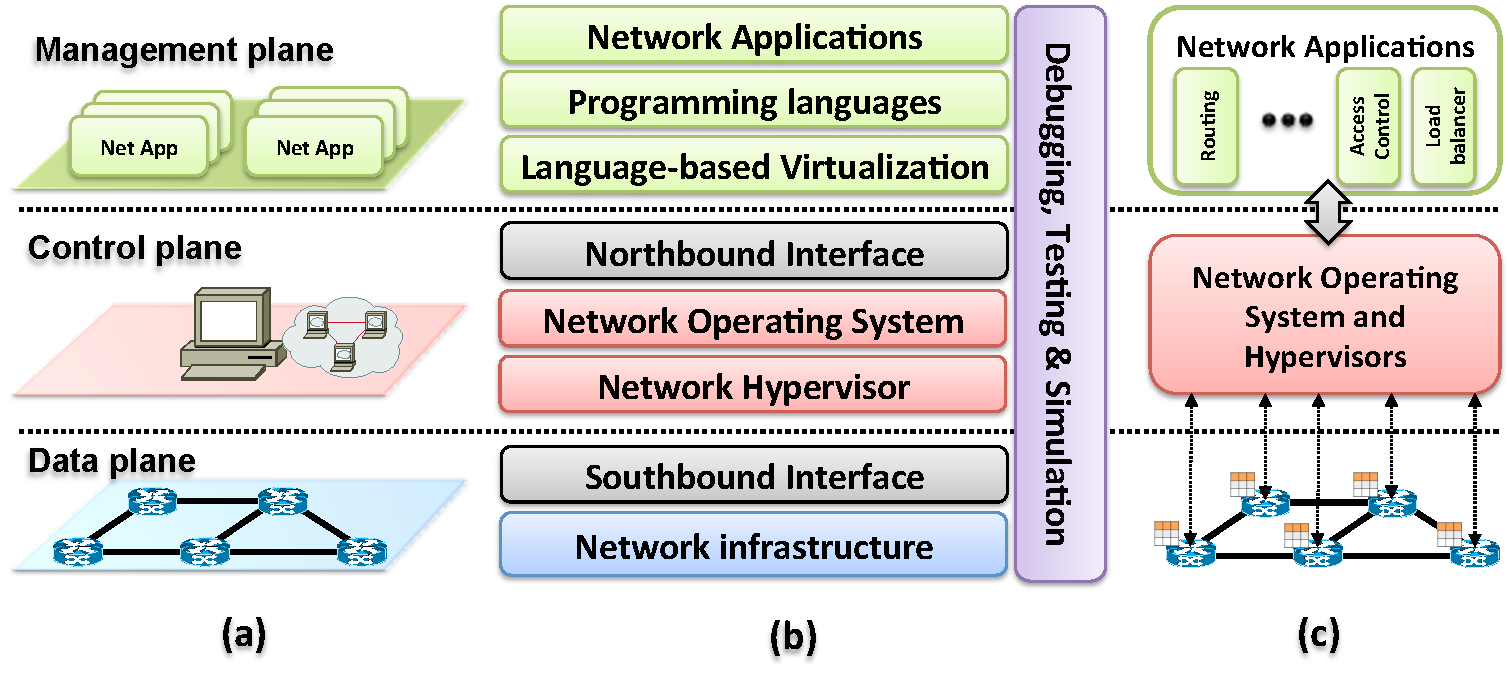
\includegraphics[width=0.85\textwidth]{figures/fig5_sdn_in_layers.pdf}
\caption{Software-Defined Networks in (a) planes, (b) layers, and (c) system design architecture}
\label{fig:sdnlayers}
\end{figure*}

Figure~\ref{fig:sdnlayers} presents a tri-fold perspective of SDNs. The SDN layers are represented 
in the center (b) of the figure, as explained above. Figures~\ref{fig:sdnlayers} (a) and ~\ref{fig:sdnlayers} (c) depict
a plane-oriented view and a system design perspective, respectively.

The following sections introduce each layer, following a bottom-up approach. For each layer, the core properties and concepts are explained based on the different technologies and solutions.  Additionally, debugging and troubleshooting techniques and tools are discussed.

\subsection{Layer I: Infrastructure}
\label{sec:infrastructure}

An SDN infrastructure, similarly to a traditional network, is composed of a set of networking 
equipment (switches, routers and middlebox appliances). The main difference resides in 
the fact that those traditional physical devices are now simple forwarding elements 
without embedded control or software to take autonomous decisions. The network intelligence is 
removed from the data plane devices to a logically-centralized control system, i.e., the network 
operating system and applications, as shown in Figure ~\ref{fig:sdnlayers} (c).
More importantly, these new networks are built (conceptually) on top of open and standard 
interfaces (e.g., OpenFlow), a crucial approach for ensuring  configuration and communication 
compatibility and interoperability among different data and control plane devices. In other words, 
these open interfaces enable controller entities to dynamically program heterogeneous forwarding 
devices, something difficult in traditional networks, due to the large variety of 
proprietary and closed interfaces and the distributed nature of the control plane.

In an SDN/OpenFlow architecture, there are two main elements, the controllers and the forwarding 
devices, as shown in Figure~\ref{fig:sdnopenflowswitch}. A data plane device is a hardware or software 
element specialized in packet forwarding, while a controller is a software stack (the ``network brain'') 
running on a commodity hardware platform. An OpenFlow-enabled forwarding device is based on a pipeline of 
flow tables where each entry of a flow table has three parts: (1) a matching rule, (2) actions to be executed 
on matching packets, and (3) counters that keep statistics of matching packets. This high-level and simplified model derived from OpenFlow is currently  the most widespread design of SDN data plane devices. Nevertheless, other specifications of SDN-enabled forwarding devices are being pursued, including POF~\cite{song2013,song2013-1} and the  Negotiable Datapath Models (NDMs) from the ONF Forwarding Abstractions Working Group (FAWG)~\cite{onf2013}.

\begin{figure*}[ht!]
\centering
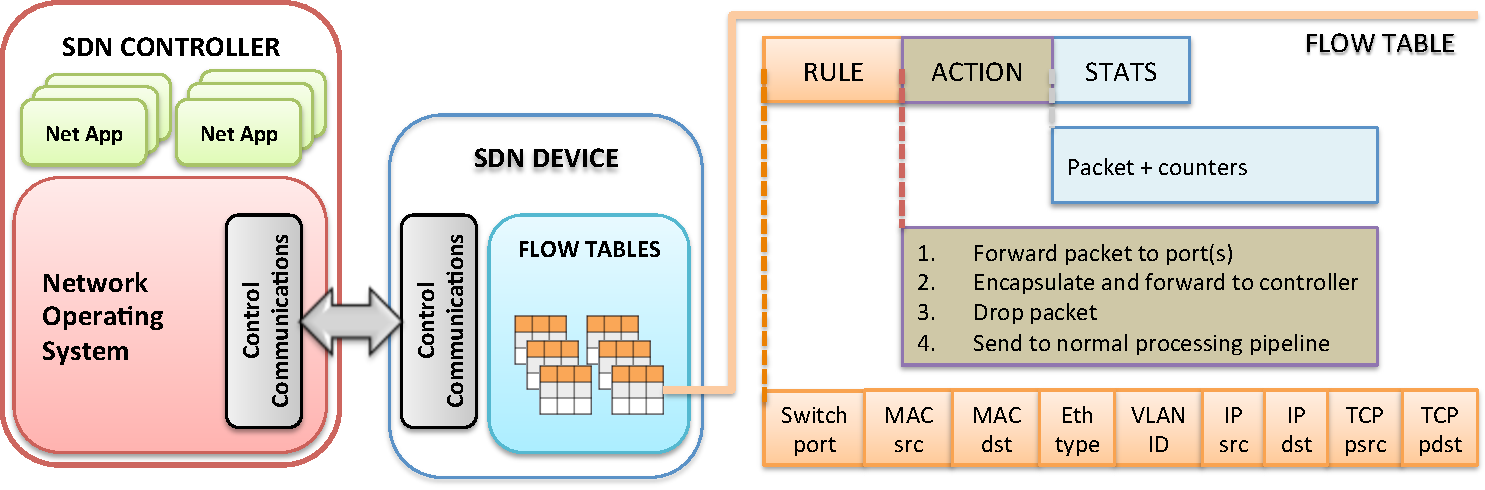
\includegraphics[width=0.85\textwidth]{figures/fig6_sdn_devices_openflow.pdf}
\caption{OpenFlow-enabled SDN devices}
\label{fig:sdnopenflowswitch}
\end{figure*}

Inside an OpenFlow device, a path through a sequence of flow tables defines how packets should be handled. 
When a new packet arrives, the lookup process starts in the first table and ends either with a match in one of the tables of the pipeline 
or with a miss (when no rule is found for that packet). 
A flow rule can be defined by combining different matching fields, as illustrated in Figure~\ref{fig:sdnopenflowswitch}.
If there is no default 
rule, the packet will be discarded. However, the common case is to install a default rule which tells the switch to send the packet to the controller (or to the normal non-OpenFlow pipeline of the switch). The priority  of the rules follows the natural sequence number of the tables and the row order in a 
flow table. Possible actions include (1) forward the packet to outgoing port(s), (2) 
encapsulate it and forward it to the controller, (3) drop it, (4) send it to the 
normal processing pipeline, (5) send it to the next flow table or to special tables, such as group or metering tables introduced in the latest OpenFlow protocol.
% versions 1.1 and 1.3, respectively.

As detailed in Table~\ref{tab:of-versions}, each version of the OpenFlow specification introduced new match fields including Ethernet, IPv4/v6, MPLS, TCP/UDP, etc. However, only a subset of those matching fields are mandatory to be compliant to a given protocol version. Similarly, many actions and port types are optional features. 
Flow match rules can be based on almost arbitrary combinations of bits of the different packet headers using bit masks for each field. Adding new matching fields has been eased with the extensibility capabilities introduced in OpenFlow version 1.2 through an OpenFlow Extensible Match (OXM) based on type-length-value (TLV) structures. To improve the overall protocol extensibility, with OpenFlow version 1.4 TLV structures have been also added to  ports, tables, and queues in replacement of the hard-coded counterparts of earlier protocol versions. 
%This provides flexibility and allows new addressing schemes on OpenFlow-enabled 
%networks, a fact that can arguably foster the development and experimentation of new 
%networking architectures and protocols, such as information and content centric networks~\cite{xxx-sdn-icn-ccn}.


{\renewcommand{\arraystretch}{1.4}
\begin{table*}[ht!]
\caption{Different match fields, statistics and capabilities have been added on each OpenFlow protocol revision. The number of required (Req) and optional (Opt) capabilities has grown considerably.}
\label{tab:of-versions}
\begin{center}
\footnotesize
\begin{tabular}{|c|l|l|c|c|c|c|c|c|c|c|}
\hline
\multirow{2}{*}{\textbf{OpenFlow Version}}        & \multirow{2}{*}{\textbf{Match fields}}           & \multirow{2}{*}{\textbf{Statistics}} & \multicolumn{2}{l|}{\textbf{\# Matches}}           & \multicolumn{2}{l|}{\textbf{\# Instructions}}    & \multicolumn{2}{l|}{\textbf{\# Actions}}          & \multicolumn{2}{l|}{\textbf{\# Ports}}           \\ \cline{4-11} 
                         &                                         &                             & Req                 & Opt                 & Req                & Opt                & Req                & Opt                 & Req                & Opt                \\ \hline  \hline
\multirow{4}{*}{v 1.0} & Ingress Port                            & Per table statistics        & \multirow{4}{*}{18} & \multirow{4}{*}{2}  & \multirow{4}{*}{1} & \multirow{4}{*}{0} & \multirow{4}{*}{2} & \multirow{4}{*}{11} & \multirow{4}{*}{6} & \multirow{4}{*}{2} \\ \cline{2-3}
                         & Ethernet: src, dst, type, VLAN                & Per flow statistics         &                     &                     &                    &                    &                    &                     &                    &                    \\ \cline{2-3}
                         & IPv4: src, dst, proto, ToS              & Per port statistics         &                     &                     &                    &                    &                    &                     &                    &                    \\ \cline{2-3}
                         & TCP/UDP: src port, dst port             & Per queue statistics        &                     &                     &                    &                    &                    &                     &                    &                    \\ \hline
\multirow{2}{*}{v 1.1} & Metadata, SCTP,  VLAN tagging       & Group statistics            & \multirow{2}{*}{23} & \multirow{2}{*}{2}  & \multirow{2}{*}{0} & \multirow{2}{*}{0} & \multirow{2}{*}{3} & \multirow{2}{*}{28} & \multirow{2}{*}{5} & \multirow{2}{*}{3} \\ \cline{2-3}
                         & MPLS: label, traffic class              & Action bucket statistics    &                     &                     &                    &                    &                    &                     &                    &                    \\ \hline
\multirow{2}{*}{v 1.2} & OpenFlow Extensible Match (OXM)         &                             & \multirow{2}{*}{14} & \multirow{2}{*}{18} & \multirow{2}{*}{2} & \multirow{2}{*}{3} & \multirow{2}{*}{2} & \multirow{2}{*}{49} & \multirow{2}{*}{5} & \multirow{2}{*}{3} \\ \cline{2-3}
                         & IPv6: src, dst, flow label, ICMPv6      &                             &                     &                     &                    &                    &                    &                     &                    &                    \\ \hline
\multirow{2}{*}{v 1.3} & \multirow{2}{*}{PBB, IPv6 Extension Headers} & Per-flow meter              & \multirow{2}{*}{14} & \multirow{2}{*}{26} & \multirow{2}{*}{2} & \multirow{2}{*}{4} & \multirow{2}{*}{2} & \multirow{2}{*}{56} & \multirow{2}{*}{5} & \multirow{2}{*}{3} \\ \cline{3-3}
                         &                                         & Per-flow meter band         &                     &                     &                    &                    &                    &                     &                    &                    \\ \hline
\multirow{2}{*}{v 1.4} & \multirow{2}{*}{---} & ---            & \multirow{2}{*}{\textbf{14}} & \multirow{2}{*}{\textbf{27}} & \multirow{2}{*}{\textbf{2}} & \multirow{2}{*}{\textbf{4}} & \multirow{2}{*}{\textbf{2}} & \multirow{2}{*}{\textbf{57}} & \multirow{2}{*}{\textbf{5}} & \multirow{2}{*}{\textbf{3}} \\ \cline{3-3}
                         &                                         & Optical port properties        &                     &                     &                    &                    &                    &                     &                    &                    \\ \hline
\end{tabular}
\end{center}
\end{table*}
}

%\vspace{2mm}
%\noindent \textit{More on OpenFlow devices}
%
%OpenFlow devices have a flow table that is configured by an external controller.
%Flow table entries are represented by rules consisting of a pattern and an action.
%A pattern can be any sequence of bits on the packet header.
%There is no strict definition of a specific address space like in IP networks, for instance.
%Additionally, rules have also an expiration time (timeout) and associated counters.
%Timeouts can be used to autonomously (by the switch itself) remove a rule from the flow table without requiring any interaction with a controller.
%There are several counters defined in the OpenFlow specification~\cite{theopennetworkingfoundation2012}.
%They can be used to collect diverse statistics from networking devices in a per flow basis.
%
%Rules can also have different granularity levels for matching the incoming flows.
%At the lowest level, a micro flow rule will match on all fields of the incoming packets.
%On the opposite side, a macro flow rule (or wildcard) can suppress (avoid matching) any number of bits in some fields.
%Therefore, it is up to the operator to define the required level of granularity.
%For instance, applications can use more than one level of granularity to solve different kinds of problems.
%While wildcards can be applied for an initial macro load balancing of incoming requests, micro flow rules may be needed to keep ongoing connection or to do finer traffic engineering when bottlenecks are close to happening.

\vspace{2mm}
\noindent \textit{Overview of available OpenFlow devices}

%At the date of this writing, 
Several OpenFlow-enabled forwarding devices are available on 
the market, both as commercial and open source products (see Table~\ref{tab:openflowdevices}).
There are many off-the-shelf, ready to deploy, OpenFlow switches and routers, among other appliances.
%A more complete list of commercially available products can be found at ~\cite{sdncentral2013}.
%Moreover, many companies have already announced new OpenFlow products~\cite{sdncentralcommunity2013}.
Most of the switches available on the market have relatively small Ternary Content-Addressable Memory (TCAMs), with up to 8K entries. 
Nonetheless, this is changing at a fast pace. Some of the latest devices released in the market go 
far beyond that figure. Gigabit Ethernet switches for common business purposes are already supporting up 
to 32K L2+L3 or 64K L2/L3 exact match flows~\cite{centecnetworks2013-1}. Enterprise class 10GE switches 
are being delivered with more than 80K Layer 2 flow entries~\cite{nec2013-1}. Other switching 
devices using high performance chips such as the EZchip NP-4, provide optimized TCAM memory that 
already supports from 125K up to 1000K flow table entries~\cite{noviflow2013-1}. This is a clear sign that the size 
of the flow tables is growing at a pace aiming to meet the needs of future SDN deployments.

Networking hardware manufacturers have produced various kinds of OpenFlow-enabled devices, as is shown in Table~\ref{tab:openflowdevices}. 
These devices range from equipment for small businesses (e.g., Gigabit Ethernet switches) to high-class data center equipment (e.g., high-density switch chassis with up to 100GbE connectivity for edge-to-core applications, with tens of Tbps of switching capacity).

{\renewcommand{\arraystretch}{1.4}
\begin{table*}[!htp]
\caption{OpenFlow enabled hardware and software devices}
\label{tab:openflowdevices}
\begin{center}
\footnotesize
%\rowcolors{1}{lightgray}{white}
\begin{tabularx}{\linewidth}{p{1.2cm}p{3.1cm}p{0.9cm}p{2.4cm}p{0.8cm}X}
\hline
\textbf{Group} & \textbf{Product} & \textbf{Type} & \textbf{Maker/Developer} & \textbf{Version} & \textbf{Short description} \\
\hline
\multirow{16}{*}{Hardware} 
& 8200zl and 5400zl~\cite{hp2013} & chassis & Hewlett-Packard & v1.0 & Data center class chassis (switch modules). \\\cline{2-6}
& Arista 7150 Series~\cite{aristanetworks2013} & switch & Arista Networks & v1.0 & Data centers hybrid Ethernet/OpenFlow switches. \\\cline{2-6}
& BlackDiamond X8~\cite{extremenetworks2013} & switch & Extreme Networks & v1.0 & Cloud-scale  hybrid Ethernet/OpenFlow switches. \\\cline{2-6}
& CX600 Series~\cite{co.2013} & router & Huawei & v1.0 & Carrier class MAN routers. \\\cline{2-6}
& EX9200 Ethernet~\cite{junipernetworks2013} & chassis & Juniper & v1.0 & Chassis based switches for cloud data centers. \\\cline{2-6}
& EZchip NP-4~\cite{yokneam2011} & chip & EZchip Technologies & v1.1 & High performance 100-Gigabit network processors. \\\cline{2-6}
& MLX Series~\cite{brocade2013} & router & Brocade & v1.0 & Service providers and enterprise class routers. \\\cline{2-6}
& NoviSwitch 1248~\cite{noviflow2013-1} & switch & NoviFlow & v1.3& High performance OpenFlow switch. \\\cline{2-6}
& NetFPGA~\cite{netfpga2014} & card & NetFPGA & v1.0 & 1G and 10G OpenFlow implementations. \\\cline{2-6}
& RackSwitch G8264~\cite{ibm2013} & switch & IBM & v1.0 & Data center switches supporting Virtual Fabric and OpenFlow. \\\cline{2-6}
& PF5240 and PF5820~\cite{nec2013-2} & switch & NEC & v1.0 & Enterprise class hybrid Ethernet/OpenFlow switches. \\\cline{2-6}
& Pica8 3920~\cite{pica8opennetworking2013} & switch & Pica8 & v1.0 & Hybrid Ethernet/OpenFlow switches. \\\cline{2-6}
& Plexxi Switch 1~\cite{plexxi2013} & switch & Plexxi & v1.0 & Optical multiplexing interconnect for data centers. \\\cline{2-6}
& V330 Series~\cite{centecnetworks2013} & switch & Centec Networks & v1.0 & Hybrid Ethernet/OpenFlow switches. \\\cline{2-6}
& Z-Series~\cite{cyan2013} & switch & Cyan & v1.0 & Family of packet-optical transport platforms.\\
\hline
\multirow{9}{*}{Software} 
& contrail-vrouter~\cite{networks2013} & vrouter &  Juniper Networks & v1.0 & Data-plane function to interface with a VRF.\\\cline{2-6}
& LINC~\cite{flowforwarding2013,rutka2013} & switch &  FlowForwarding & v1.3 & Erlang-based soft switch with OF-Config 1.1 support.\\\cline{2-6}
& ofsoftswitch13~\cite{cpqd2013} & switch & Ericsson, CPqD & v1.3 & OF 1.3 compatible user-space software switch implementation. \\\cline{2-6}
& Open vSwitch~\cite{listofcontributors2013,pfaff2009} & switch & Open Community & v1.0  & Switch platform designed for virtualized server environments.  \\\cline{2-6}
& OpenFlow Reference~\cite{openflowcommunity2009} & switch & Stanford & v1.0 & OF Switching capability to a Linux PC with multiple NICs. \\\cline{2-6}
& OpenFlowClick~\cite{mundada2009} & vrouter & Yogesh Mundada & v1.0 & OpenFlow switching element for Click software routers.\\\cline{2-6}
& Switch Light~\cite{bigswitchnetworks2013} & switch & Big Switch & v1.0  & Thin switching software platform for physical/virtual switches. \\\cline{2-6}
& Pantou/OpenWRT~\cite{yiakoumis2011} & switch & Stanford  & v1.0 & Turns a wireless router into an OF-enabled switch. \\\cline{2-6}
& XorPlus~\cite{shang2014} & switch &  Pica8 & v1.0 & Switching software for high performance ASICs.\\
\hline
\end{tabularx}
\end{center}
\end{table*}
}
%& Pica8~\cite{pica8opennetworking2013-1} & switch & Pica8 & v1.2 & Hardware independent software stack for open switches. \\\cline{2-6}
%& Indigo~\cite{projectfloodlight2013} & switch & Big Switch & v1.0 & Uses hardware features of Ethernet switch ASICs to run OF. \\\cline{2-6}
%& RouteFlow~\cite{nascimento2011} & router & CPqD & v1.0 & Virtual OpenFlow enabled routers for Internet service providers.

Software switches are emerging as one of the most promising 
solutions for data centers and virtualized network infrastructures~\cite{weissberger2013,schenker2013,casado2013}.
Examples of software-based OpenFlow switch implementations include Switch Light~\cite{bigswitchnetworks2013}, ofsoftswitch13~\cite{cpqd2013}, Open vSwitch~\cite{listofcontributors2013}, OpenFlow Reference~\cite{openflowcommunity2009}, Pica8~\cite{pica8opennetworking2013-1}, Pantou~\cite{yiakoumis2011}, and XorPlus~\cite{shang2014}.
Recent reports show that the number of virtual access ports is already larger than physical access ports on data centers~\cite{casado2013}. 
Network virtualization has been one of the drivers behind this trend.
Software switches such as Open vSwitch have been used for moving network functions to the edge (with the core performing traditional IP forwarding), thus enabling network virtualization~\cite{koponen}.

An interesting observation is the number of small, start-up enterprises devoted to SDN, such as 
Big Switch, Pica8, Cyan, Plexxi, and NoviFlow. This seems to imply that SDN is springing a more competitive and open 
networking market, one of its original goals.
Other effects of this openness triggered by SDN include the emergence of so-called ``bare metal switches'' or ``whitebox switches'', where the software and hardware are sold separately and the end-user is free to load an operating system of its choice~\cite{onie2013}. 

%%Moreover, customers have been waiting for a long time new
%%technologies for creating new conditions to drive innovation and new
%%opportunities in the ``locked down'' network world, i.e., more less
%%inflexible network infrastructures and a %%market (hard to compete
%%in) traditionally owned and controlled by a few big companies.

\subsection{Layer II: Southbound Interfaces}
\label{sec:southboundAPIs}
% FIXME: extract and put forward the essential properties of southbound APIs

Southbound interfaces (or southbound APIs) are the connecting bridges between control and forwarding 
elements, thus being the crucial instrument for clearly separating control and data plane functionality. However, 
these APIs are still tightly tied to the forwarding elements of the underlying physical or virtual 
infrastructure.

Typically, a new switch can take two years to be ready for commercialization if built from scratch, 
with upgrade cycles that can take up to nine months. The software development for a new product can 
take from six months to one year~\cite{kato2013}. The initial investment 
is high and risky. 
As a central component of its design the southbound APIs represent one of the major barriers for the introduction 
and acceptance of any new networking technology. 
In this light, the emergence of SDN southbound API proposals such as OpenFlow~\cite{mckeown2008} is seen as welcome by many in the industry.
These standards promote interoperability, allowing the deployment of vendor-agnostic network devices. 
This has already been demonstrated by the interoperability between OpenFlow-enabled equipments from different vendors.

As of this writing, OpenFlow is the most widely accepted and deployed open southbound standard 
for SDN. It provides a common specification to implement OpenFlow-enabled forwarding devices, and for the
communication channel between data and control plane devices (e.g., switches and controllers).
%An OpenFlow-enabled switch is similar to a normal Ethernet device, except that it does not act 
%autonomously. Actually, since the OpenFlow 1.1.0 specification~\cite{onf2012}, 
%there is a standalone operation mode, which can be enabled when the connection with the controller 
%fails. In this case, the device will act exactly as an Ethernet switch. Apart from exceptional 
%situations, an OpenFlow device will look for a matching rule in the local flow tables for every 
%incoming packet. A positive match tells the device what to do with the ingress packet, i.e., which 
%actions to take.
The OpenFlow protocol provides three information sources for network operating systems.
First, event-based messages are sent by forwarding devices to the controller when a link or port 
change is triggered. Second, flow statistics are generated by the forwarding devices and collected 
by the controller. Third, packet-in messages are sent by forwarding devices to the controller when 
they do not known what to do with a new incoming flow or because there is an explicit ``send to 
controller'' action in the matched entry of the flow table. These information channels are the essential 
means to provide flow-level information to the network operating system.

Albeit the most visible, OpenFlow is not the only available southbound interface for SDN.
There are other API proposals such as ForCES~\cite{doria2010}, OVSDB~\cite{pfaff2013-1}, POF~\cite{song2013,song2013-1}, and OpFlex~\cite{smith2014}.
ForCES proposes a more flexible approach to traditional network management without changing the current architecture of the network, i.e., without the need of a logically-centralized external controller. 
The control and data planes are separated but can potentially be kept in the same network element.
However, the control part of the network element can be upgraded on-the-fly with third-party firmware.
%, for instance.

%Interestingly, despite ForCES being older than OpenFlow, it is not yet widely accepted or supported on commercial products.
%Nevertheless, this does not mean its end because we are only on the early chapters of SDN.
%There is plenty space and opportunity for new southbound APIs.
%History has shown us that different environments, requirements and market needs are some of the major driving forces for developing new technologies and solutions.

OVSDB~\cite{pfaff2013-1} is another type of southbound API, designed to provide 
advanced management capabilities for Open vSwitches. Beyond OpenFlow's capabilities to configure 
the behavior of flows in a forwarding device, an Open vSwitch offers other networking functions.
For instance, it allows the control elements to create multiple virtual switch instances, set QoS 
policies on interfaces, attach interfaces to the switches, configure tunnel interfaces on OpenFlow 
data paths, manage queues, and collect statistics.
Therefore, the OVSDB is a complementary protocol to OpenFlow for Open vSwitch. 


%OpenSketch~\cite{yu2013-1} is an example of a more specific southbound API.
%It proposes data and control plane abstractions specifically for measurement purposes.
%One of the goals of OpenSketch is to allow multiple measurement tasks to execute concurrently without impairing accuracy.
%
%The internal design of a OpenSketch switch can be seen as a pipeline with three stages (hashing, classification, counting).
%Input packets have to first pass through a hashing function.
%Then they are classified accordingly a matching rule.
%Lastly, the match rule identifies a counting index, which is used to calculate the counter location in the counting stage.
%While a TCAM with few entries is enough for stage two (classification rules), the flexible counters are stored in SRAM.
%This makes the OpenSketch's operation efficient (fast matching) and costly effectively (cheaper SRAMs to store counters).
%However, differently from OpenFlow, OpenSketch is a special purpose southbound API designed to provide flexibility for measurements.
%\note{DK: Maybe, move to another place --- monitoring, applications, etc.}

One of the first direct competitors of OpenFlow is POF~\cite{song2013,song2013-1}.
One of the main goals of POF is to enhance the current SDN forwarding plane.
With OpenFlow, switches have to understand the protocol headers to extract the required bits to be matched with the flow tables entries.
This parsing represents a significant burden for data plane devices, in particular if we consider that OpenFlow version 1.3 already contains more  than 40 header fields. 
Besides this inherent complexity, backward compatibility issues may arise every time new header fields are included in or removed from the protocol.
To achieve its goal, POF proposes a generic flow  instruction set (FIS) that makes the forwarding plane protocol-oblivious.
A forwarding element does not need to know, by itself, anything about the packet format in advance.
Forwarding devices are seen as white boxes with only processing and forwarding  capabilities. 
In POF, packet parsing is a controller task that results in a sequence of generic keys and table lookup instructions that are installed in the forwarding elements.
The behavior of data plane devices is therefore completely under the control of the SDN controller.
Similar to a CPU in a computer sytem, a POF switch is application- and protocol-agnostic. 

A very recent soutbound interface proposal is OpFlex~\cite{smith2014}.
Contrary to OpenFlow (and similar to ForCES), one of the ideas behind OpFlex is to distribute part of the 
complexity of managing the network back to the forwarding devices, with the aim of improving scalability.
Similar to OpenFlow, policies are logically centralized and abstracted from the underlying implementation.
The differences between OpenFlow and OpFlex are a clear illustration of one of the important questions to be answered when devising a southbound interface: where to place each piece of the overall functionality. 

\subsection{Layer III: Network Hypervisors}
\label{sec:virtualizationhypervisor}

Virtualization is already a consolidated technology in modern computers. The fast 
developments of the past decade have made virtualization of computing platforms mainstream.
Based on recent reports, the number of virtual servers has already exceeded the number of physical 
servers~\cite{bittman2013,koponen}.

Hypervisors enable distinct virtual machines to share the same hardware resources. In a 
cloud infrastructure-as-a-service (IaaS), each user can have its own virtual resources, from computing to 
storage. This enabled new revenue and business models where users allocate resources on-demand, from a shared 
physical infrastructures, at a relatively low cost.
% (less CAPEX and OPEX expenditures, for instance). 
At the same time, providers make better use of the capacity of their installed physical 
infrastructures, creating new revenue streams without significantly increasing their CAPEX and OPEX 
costs. One of the interesting features of virtualization technologies today is the fact that virtual 
machines can be easily migrated from one physical server to another and can 
be created and/or destroyed on-demand, enabling the provisioning of elastic services with flexible 
and easy management.
Unfortunately, virtualization has been only partially realized in practice. Despite the great advances 
in virtualizing computing and storage elements, the network is still mostly statically configured in a box-by-box manner~\cite{chowdhury2010}.

The main network requirements can be captured along two dimensions: network topology and address space.
Different workloads require different network topologies and services, such as flat L2 or L3 services, or even more complex L4-L7 
services for advanced functionality.
Currently, it is very difficult for a single physical topology to support the diverse demands 
of applications and services. Similarly, address space is hard to change in current networks. Nowadays, 
virtualized workloads have to operate in the same address of the physical infrastructure. 
Therefore, it is hard to keep the original network configuration for a tenant, virtual machines can not migrate to arbitrary locations, and the addressing scheme is fixed and hard to change. 
For example, IPv6 cannot be used by the VMs of a tenant if the underlying physical forwarding devices support only IPv4.

%It is also worth emphasizing that traditional networks have a fairly static nature and are complex to manage.
%Things such as virtualization, live network migration or network changes are yet hard to implement.
%Therefore, flexible, fast, scalable and on-demand network virtualization is still one of the major open challenges in the network world.

To provide complete virtualization the network should provide similar properties to the computing layer~\cite{chowdhury2010}.
The network infrastructure should be able to support arbitrary network topologies and addressing schemes.
Each tenant should have the ability to configure both the computing nodes and the network simultaneously.
Host migration should automatically trigger the migration of the corresponding virtual network ports.
One might think that long standing virtualization primitives such as VLANs (virtualized L2 domain), NAT (Virtualized IP address space), and 
MPLS (virtualized path) are enough to provide full and automated network virtualization.
However, these  technologies are anchored on a box-by-box basis configuration, i.e., there is no single unifying 
abstraction that can be leveraged to configure (or reconfigure) the network in a global manner.
As a consequence, current network provisioning can take months, while computing provisioning takes only 
minutes~\cite{koponen,cearley2013,peng2012,zhang2014}.

There is hope that this situation will change with SDN and the availability of new tunneling techniques (e.g., VXLAN~\cite{mahalingam2013}, NVGRE~\cite{sridharan2013}).
For instance, solutions such as FlowVisor~\cite{sherwood2009,sherwood2010,azodolmolky2012},  FlowN~\cite{drutskoy2012}, NVP~\cite{koponen}, OpenVirteX~\cite{al-shabibi2014} and IBM SDN VE~\cite{racherla2014,li2014}
have been recently proposed, evaluated and deployed in real scenarios for on-demand provisioning of virtual 
networks.

\vspace{2mm}
\noindent \textit{Slicing the network}

FlowVisor is one of the early technologies to virtualize a Software-Defined Network.
%FlowVisor is also the first known hypervisor for OpenFlow-based SDNs. 
Its basic idea is to allow multiple logical networks share the same OpenFlow networking infrastructure.
For this purpose, it provides an abstraction layer that makes it easier to slice a data plane based on off-the-shelf OpenFlow-enabled switches, allowing multiple and diverse networks to co-exist. 
%More interestingly, it works with off-the-shelf OpenFlow-enabled switches, not requiring any 
%specialized or programmable hardware such as FPGAs or specific network processors.

Five slicing dimensions are considered in FlowVisor: bandwidth, topology, traffic, device CPU and forwarding 
tables. Moreover, each network slice supports a controller, i.e., multiple controllers can co-exist on top 
of the same physical network infrastructure. Each controller is allowed to act only on its own network slice.
In general terms, a slice is defined as a particular set of flows on the data plane. 
From a system design perspective, FlowVisor is a transparent proxy that intercepts OpenFlow messages between 
switches and controllers. It partitions the link bandwidth and flow tables of each switch. Each slice receives 
a minimum data rate and each guest controller gets its own virtual flow table in the switches.

Similarly to FlowVisor, OpenVirteX~\cite{al-shabibi2014} acts as a proxy between the network operating system and the forwarding 
devices. However, its main goal is to provide virtual SDNs through both topology, address, and control function
virtualization. 
All these properties are necessary in multi-tenant environments where virtual networks 
need to be managed and migrated according to the computing and storage virtual resources. Virtual network 
topologies have to be mapped onto the underlying forwarding devices, with virtual addresses allowing tenants 
to completely manage their address space without depending on the underlying network elements addressing schemes.

AutoSlice~\cite{bozakov2012} is another SDN-based virtualization proposal. Similar to FlowVisor, the idea is to 
allow multiple controllers to manage their respective virtual SDN.
The main difference is that AutoSlice intends to develop a transparent virtualization layer, or SDN hypervisor, 
to automate the deployment of virtual SDNs in a less cumbersome manner than FlowVisor.

FlowN~\cite{drutskoy2012,drutskoy2013} is based on a slightly different concept. Whereas FlowVisor can be compared to a full virtualization technology, FlowN 
is analogous to a container-based virtualization, i.e., a lightweight virtualization approach. FlowN 
was also primarily conceived to address multi-tenancy in the context of cloud platforms. It is designed to 
be scalable and allows a unique shared controller platform to be used for managing multiple domains 
in a cloud environment. Each tenant has full control over its virtual networks and is free to deploy 
any network abstraction and application on top of the controller platform.


\vspace{2mm}
\noindent \textit{Commercial multi-tenant network hypervisors}

None of the aforementioned approaches is designed to address all challenges of multi-tenant 
data centers. For instance, tenants want to be able to migrate their enterprise solutions to cloud 
providers without the need to modify the network configuration of their home network. Existing 
networking technologies and migration strategies have mostly failed to meet both the tenant and the 
service provider requirements.
A multi-tenant environment should be anchored in a network hypervisor capable of abstracting the 
underlaying forwarding devices and physical network topology from the tenants. Moreover, each tenant 
should have access to control abstractions and manage its own virtual networks independently and 
isolated from other tenants.

With the market demand for network virtualization and the recent research on SDN showing promise as an enabling technology, different commercial virtualization platforms based on SDN concepts have started to appear.
VMWare has proposed a network virtualization platform (NVP)~\cite{koponen} that provides the necessary abstractions to allow the creation of independent virtual networks for large-scale multi-tenant environments.
NVP is a complete network virtualization solution that allows the creation of virtual networks, each with independent service model, topologies, and addressing architectures over the same physical network.
With NVP, tenants do not need to know anything about the underlying network topology, configuration or other specific aspects of the forwarding devices. 
NVP's network hypervisor translates the tenants configurations and requirements into low level instruction sets to be installed on the forwarding devices. 
For this purpose, the platform uses a cluster of SDN controllers to manipulate the forwarding tables of the Open vSwitches in the host's hypervisor. 
Forwarding decisions are therefore made exclusively on the network edge.
After the decision is made, the packet is tunneled over the physical network to the receiving host hypervisor (the physical network sees nothing but ordinary IP packets).

IBM has also recently proposed SDN VE~\cite{racherla2014,li2014}, another commercial and enterprise-class network virtualization platform.
SDN VE uses OpenDaylight as one of its building blocks for Software-Defined Environments (SDEs)\footnote{We will return to OpenDaylight and SDE later.}.
This solutions also offers a complete implementation framework for network virtualization. 
Like NVP, it uses a host-based overlay approach, achieving advanced network abstraction that enables application-level network services in large-scale multi-tenant environments. 
%It provides a multi-hypervisor, server-centric solution comprising multiple components that overlay virtual networks onto any physical network that provides IP connectivity.
Interestingly, SDN VE 1.0 is capable of supporting in one single instantiation up to 16,000 virtual networks and 128,000 virtual machines~\cite{racherla2014,li2014}.
%The overall solution is designed to support up to 16M virtual networks in a global deployment.
%distinct virtual networks for multi-tenancy separation and isolation, multicast support without needing to be supported on the underlaying %hardware.
%This gives a rough idea of what future software-defined environments will be capable of delivering for the  evolution of IT infrastructures.

To summarize, currently there are only a few network hypervisor proposals leveraging the advances of SDN.
We antecipate, however, this ecosystem to expand in the near future since network virtualization will most likely play a key role in future virtualized environments, similarly to the expansion we have been witnessing in virtualized computing.

%By providing also overlay networks for backward compatibility, SDN VE also ensures:
%scalability on  L2 and L3 independently from the underlying network infrastructure;
%reduced exposure of MAC addresses in the underlay network;
%migration capabilities across data centers using L3 without any kind of dependency on the existing underlaying L2;
%smoothly migration of workloads to any location while still retaining the physical addressing scheme, even when overlapping schemes are used;
%broadcast isolation within each DMZ; and 
%open standard integration of systems without any kind of hardware or vendor lock-in.

%As an example of its interoperability capabilities, which are embedded since its conception, SDN VE is already integrated with VMware and KVM hypervisors/technologies, as well as OpenFlow-enabled devices through the unified controller.
%Furthermore, another cornerstone of the solution is the DOVE Overlay network, which, among other things, provides backward compatibility and interoperability. 
% What is does is to create virtual networks that transparently allow VM to VM communication throughout the infrastructure, without requiring any change on existing underlay network that it rides over.
% In other words, it represents and integration for a seamless migration between current existing infrastructures and OpenFlow-enabled data planes.
% One of the key technologies used by the DOVE Overlay is the VXLAN frame format.


\subsection{Layer IV: Network Operating Systems / Controllers}
\label{sec:controllers}

Traditional operating systems provide abstractions (e.g., high-level programming APIs) for accessing 
lower-level devices, manage the concurrent access to the underlying resources (e.g., hard drive, network 
adapter, CPU, memory), and provide security protection mechanisms. These functionalities and resources 
are key enablers for increased productivity, making the life of system and application developers easier. Their 
widespread use has significantly contributed to the evolution of various ecosystems (e.g., programming 
languages) and the development of a myriad of applications.

In contrast, networks have so far been managed and configured using lower level, device-specific instruction 
sets and mostly closed proprietary network operating systems (e.g., Cisco IOS and Juniper JunOS). 
Moreover, the idea of operating systems abstracting device-specific characteristics 
and providing, in a transparent way, common functionalities is still almost absent in networks.
For instance, nowadays designers of routing protocols need to deal with complicated distributed algorithms when solving networking problems.
Network practitioners have therefore been solving the same problems over and over again.

SDN is promised to facilitate network management and ease the burden of solving networking problems by means of the logically-centralized control offered by a network operating system (NOS)~\cite{gude2008}.
As with traditional operating systems, the crucial value of a NOS is to provide abstractions, essential services, 
and common application programming interfaces (APIs) to developers. 
Generic functionality as network state and network topology information, device discovery, and distribution of network configuration can be provided as services of the NOS.
With NOSs, to define network policies a developer no longer needs to care about the low-level details of data distribution among routing elements, for instance.
Such systems can arguably create a new environment capable of fostering innovation at a faster pace by reducing the inherent complexity of creating new network protocols and management applications.

A NOS (or controller) is a critical element in an SDN architecture as it is the key supporting piece 
for the control logic (applications) to generate the network configuration based on the policies defined by the network operator. 
Similar to a traditional operating system, the control platform abstracts the lower-level details of connecting and interacting with forwarding devices (i.e., of materializing the network policies).

%\vspace{2mm}
%\noindent \textit{Inside a controller}
%
%Figure~\ref{fig:controllerarchitecture} illustrates a simplified internal architecture of a controller.
%It gives an idea of how a controller and management applications deal with requests from forwarding devices.
%Incoming requests can go simultaneously through one or more pipelines of applications.
%For instance, programming languages like Pyretic~\cite{monsanto2013} make it possible this kind of composition, allowing two distinct configurations, parallel pipelines (e.g., packets are processed at the same time by apps 3 and 4) and sequential pipelines (e.g., packets go sequentially through apps 1 and 2).
%Regardless of the set of applications and pipelines, the output is always the same, i.e., programming/configuration data or data requests to be send to the forwarding devices.
%
%\begin{figure}[ht]
%\centering
%\includegraphics[width=\columnwidth]{figures/sdn-controller-internals-v3.pdf}
%\caption{Illustrated controller internals}
%\label{fig:controllerarchitecture}
%\end{figure}
%
%However, each controller can have a specific internal architecture that depends on design, development and technology choices with its inherent constraints.
%While some controllers have flow processing pipelines and are able to handle applications in parallel, others allow only a more static and sequential combination of applications.
%Controllers are also designed to explore two kinds of parallelism, on the application level and on the flow processing capabilities.
%Therefore, in some controllers even a single application pipeline may have concurrent instances for higher throughput, for instance.
%Moreover, there are controllers that have additional mechanisms to deal with concurrency problems such as packets/requests issued by a switch for a flow that is already in a configuration process.
%These kind of requests/packets can be automatically discharged by the controller.
%
%% FIXME: look for the best place to introduce these practical aspects of OpenFlow controllers
%In practical terms, the three top features in most OpenFlow controllers are:
%\begin{enumerate}
%\item \textit{Event-driven model}: each module registers listeners or call-back functions (example of async events include PACKET\_IN, PORT\_STATUS, FEATURE\_REPLY, STATS\_REPLY).
%\item \textit{Packet parsing capabilities}: when switch sends an OpenFlow message, module extracts relevant information using standard procedures.
%\item \textit{switch.send(msg)}, where msg can be
%  \begin{itemize}
%  \item PACKET\_OUT with buffer\_id or fabricated packet
%  \item FLOW\_MOD with match rules and action taken
%  \item FEATURE\_REQUEST, STATS\_REQUEST, BARRIER\_REQUEST
%  \end{itemize}
%\end{enumerate}
%


\vspace{2mm}
\noindent \textit{Architecture and design axes}
\vspace{2mm}

%While a controller can be seen as the kernel of an operating system, a control platform can be viewed as an operating system distribution (e.g., Ubuntu Linux).
There are very diverse controllers and control platforms with different design and architectural choices~\cite{koponen-1,opendaylight2013,junipernetworks2013-1,hp2013-1,phemius2013,erickson2013-1}.
Existing controllers can be categorized based on many aspects. 
From an architectural point of view, one of the most relevant is if they are centralized or distributed.
This is one of the key design axes of SDN control platforms, so we start by discussing this aspect next. 

\vspace{2mm}
\noindent \textit{Centralized vs. Distributed}

A centralized controller  is a single entity that manages all forwarding devices of the network.
Naturally, it represents a single point of failure and may have scaling limitations.
A single controller may not be enough to manage a network with a large number of data plane elements. 
Centralized controllers such as NOX-MT ~\cite{tootoonchian2012},
Maestro~\cite{cai2011}, Beacon~\cite{erickson2013}, and Floodlight~\cite{openflowhub.org2012}    
have been designed as highly concurrent systems, to achieve the throughput required by enterprise class 
networks and data centers. 
These controllers are based on multi-threaded designs to explore the parallelism of multi-core computer architectures.
As an example, Beacon can deal with more than 12 
million flows per second by using large size computing nodes of cloud providers such as Amazon~\cite{erickson2013}. Other centralized controllers such as Trema~\cite{takamiya2012}, 
Ryu NOS~\cite{nippontelegraphandtelephonecorporation2012}, Meridian~\cite{banikazemi2013}, and 
ProgrammableFlow~\cite{nec2013,nec2013-2} target more or less 
specific environments such as data centers, cloud infrastructures, and carrier grade networks.

Contrary to a centralized design, a distributed network operating system can be scaled up to meet the requirements 
of potentially any environment, from small to large-scale networks.
A distributed controller can be 
a centralized cluster of nodes or a physically distributed set of elements. While the first alternative 
can offer high throughput for very dense data centers, the latter can be more resilient to different 
kinds of logical and physical failures.
A cloud provider that spans multiple data centers interconnected by a wide area network may require a hybrid approach, with clusters of controllers inside each data center and 
distributed controller nodes in the different sites~\cite{jain2013-1}.

Onix~\cite{koponen-1}, HyperFlow~\cite{tootoonchian2010},
HP VAN SDN~\cite{hp2013-1}, ONOS~\cite{krishnaswamy2013}, DISCO~\cite{phemius2013},
and \textit{yanc}~\cite{monaco2013} are examples of distributed controllers. 
Most distributed controllers offer weak consistency semantics, which means that data updates on distinct nodes will \emph{eventually} be updated on 
all controller nodes.
This implies that there is a period of time in which distinct nodes may read different 
values (old value or new value) for a same property.
Strong consistency, on the other hand, ensures that all 
controller nodes will read the most updated property value after a write operation.
Despite its impact on system performance, strong consistency offers a simpler interface to application developers.
To date, only Onix and ONOS provide different data consistency models (both weak and strong). 

%A developer implementing an application for a system which offers only weak consistency has to be 
%aware of the fact that reading values of properties in different controlling node can produce different 
%outputs, i.e., lead to eventual data inconsistencies in the application if it has not been carefully designed 
%and implemented.

Another common property of distributed controllers is fault tolerance.
When one node fails, another neighbor node should take over the duties and devices of the failed node. 
So far, despite some controllers tolerating crash failures, they do not tolerate
arbitrary failures, which means that any node with an abnormal behavior will not be replaced by a potentially 
well behaved one.

%The robustness of control platforms varies, depending on whether they are centralized or distributed.
A single controller may be enough to manage a small network, however it represents a single point 
of failure.
Similarly, independent controllers can be spread across the network, each of them managing 
a network segment, reducing the impact of a single controller failure. Yet, if the control plane
availability is critical, a cluster of controllers can be used to achieve a higher degree of availability 
and/or for supporting more devices.
Ultimately, a distributed controller can improve the control plane 
resilience, scalability and reduce the impact of problems caused by network partition, for instance.
SDN resiliency as a whole is an open challenge that will be further discussed in Section \ref{sec:resiliency}.

\vspace{2mm}
\noindent \textit{Dissecting SDN Controller Platforms}
%\noindent \textit{Layering the Controller Platform}
%\noindent \textit{Sublayers of a Controller Platform}
\vspace{2mm}


To provide a better architectural overview and understanding the design a network operating system, Table~\ref{tab:controllerdesign} summarizes some of the most relevant architectural and design properties of 
SDN controllers and control platforms. 
We have focused on the elements, services and interfaces of a selection of production-level, well-documented controllers and control platforms.
Each line in the table represent a component we consider important in a modular and scalable control platform.
We observe a highly diversified environment, with different properties and components being used by distinct control platforms.
This is not surprising, given an environment with many competitors willing to be at the forefront of SDN development.
Note also that not all components are available on all platforms.
For instance, east/westbound APIs are not required in centralized controllers such as Beacon. 
In fact, some platforms have very specific niche markets, such as telecom companies and cloud providers, so the requirements will be different.


{\renewcommand{\arraystretch}{1.4}
\begin{table*}[!htp]
\caption{Architecture and design elements of control platforms}
\label{tab:controllerdesign}
\begin{center}
\footnotesize
\begin{tabularx}{\textwidth}{|p{1.9cm}|X|X|X|X|X|}
\hline
\textbf{Component} & \textbf{OpenDaylight} & \textbf{OpenContrail} & \textbf{HP VAN SDN} & \textbf{Onix} & \textbf{Beacon} \\\hline

\textbf{Base network services}     & Topology/Stats/Switch Manager, Host Tracker, Shortest Path Forwarding & Routing, Tenant Isolation & Audit Log, Alerts, Topology, Discovery & Discovery, Multi-consistency Storage, Read State, Register for updates  & Topology, device manager, and routing \\\hline

\textbf{East/Westbound APIs}       & \textit{---} & Control Node (XMPP-like control channel) & Sync API & Distribution I/O module & \textit{Not present} \\\hline

\textbf{Integration Plug-ins}  & OpenStack Neutron & CloudStack, OpenStack & OpenStack & \textit{---} & \textit{---} \\\hline

\textbf{Management Interfaces} & GUI/CLI, REST API & GUI/CLI & REST API Shell / GUI Shell & \textit{---} & Web \\\hline

\textbf{Northbound APIs}           & REST, RESTCONF, Java APIs & REST APIs (configuration, operational, and analytic) & REST API, GUI Shell & Onix API (general purpose) & API (based on OpenFlow events) \\\hline

\textbf{Service abstraction layers} & Service Abstraction Layer (SAL) & \textit{---} & Device Abstraction API & Network Information Base (NIB) Graph with Import/Export Functions & \textit{---} \\\hline

\textbf{Southbound APIs or connectors} & OpenFlow, OVSDB, SNMP, PCEP, BGP, NETCONF & \textit{---} & OpenFlow, L3 Agent, L2 Agent & OpenFlow, OVSDB & OpenFlow \\\hline

\end{tabularx}
\end{center}
\end{table*}
}


Based on the analysis of the different SDN controllers proposed to date (both those presented in Table~\ref{tab:controllerdesign} and others, such as NOX~\cite{gude2008}, Meridian~\cite{banikazemi2013}, ForCES~\cite{doria2010}, and  FortNOX~\cite{porras2012}), we extract several common elements and provide a first attempt to clearly and systematically dissect an SDN control platform in Figure~\ref{fig:controlplatformarch}.

\begin{figure*}[ht]
\centering
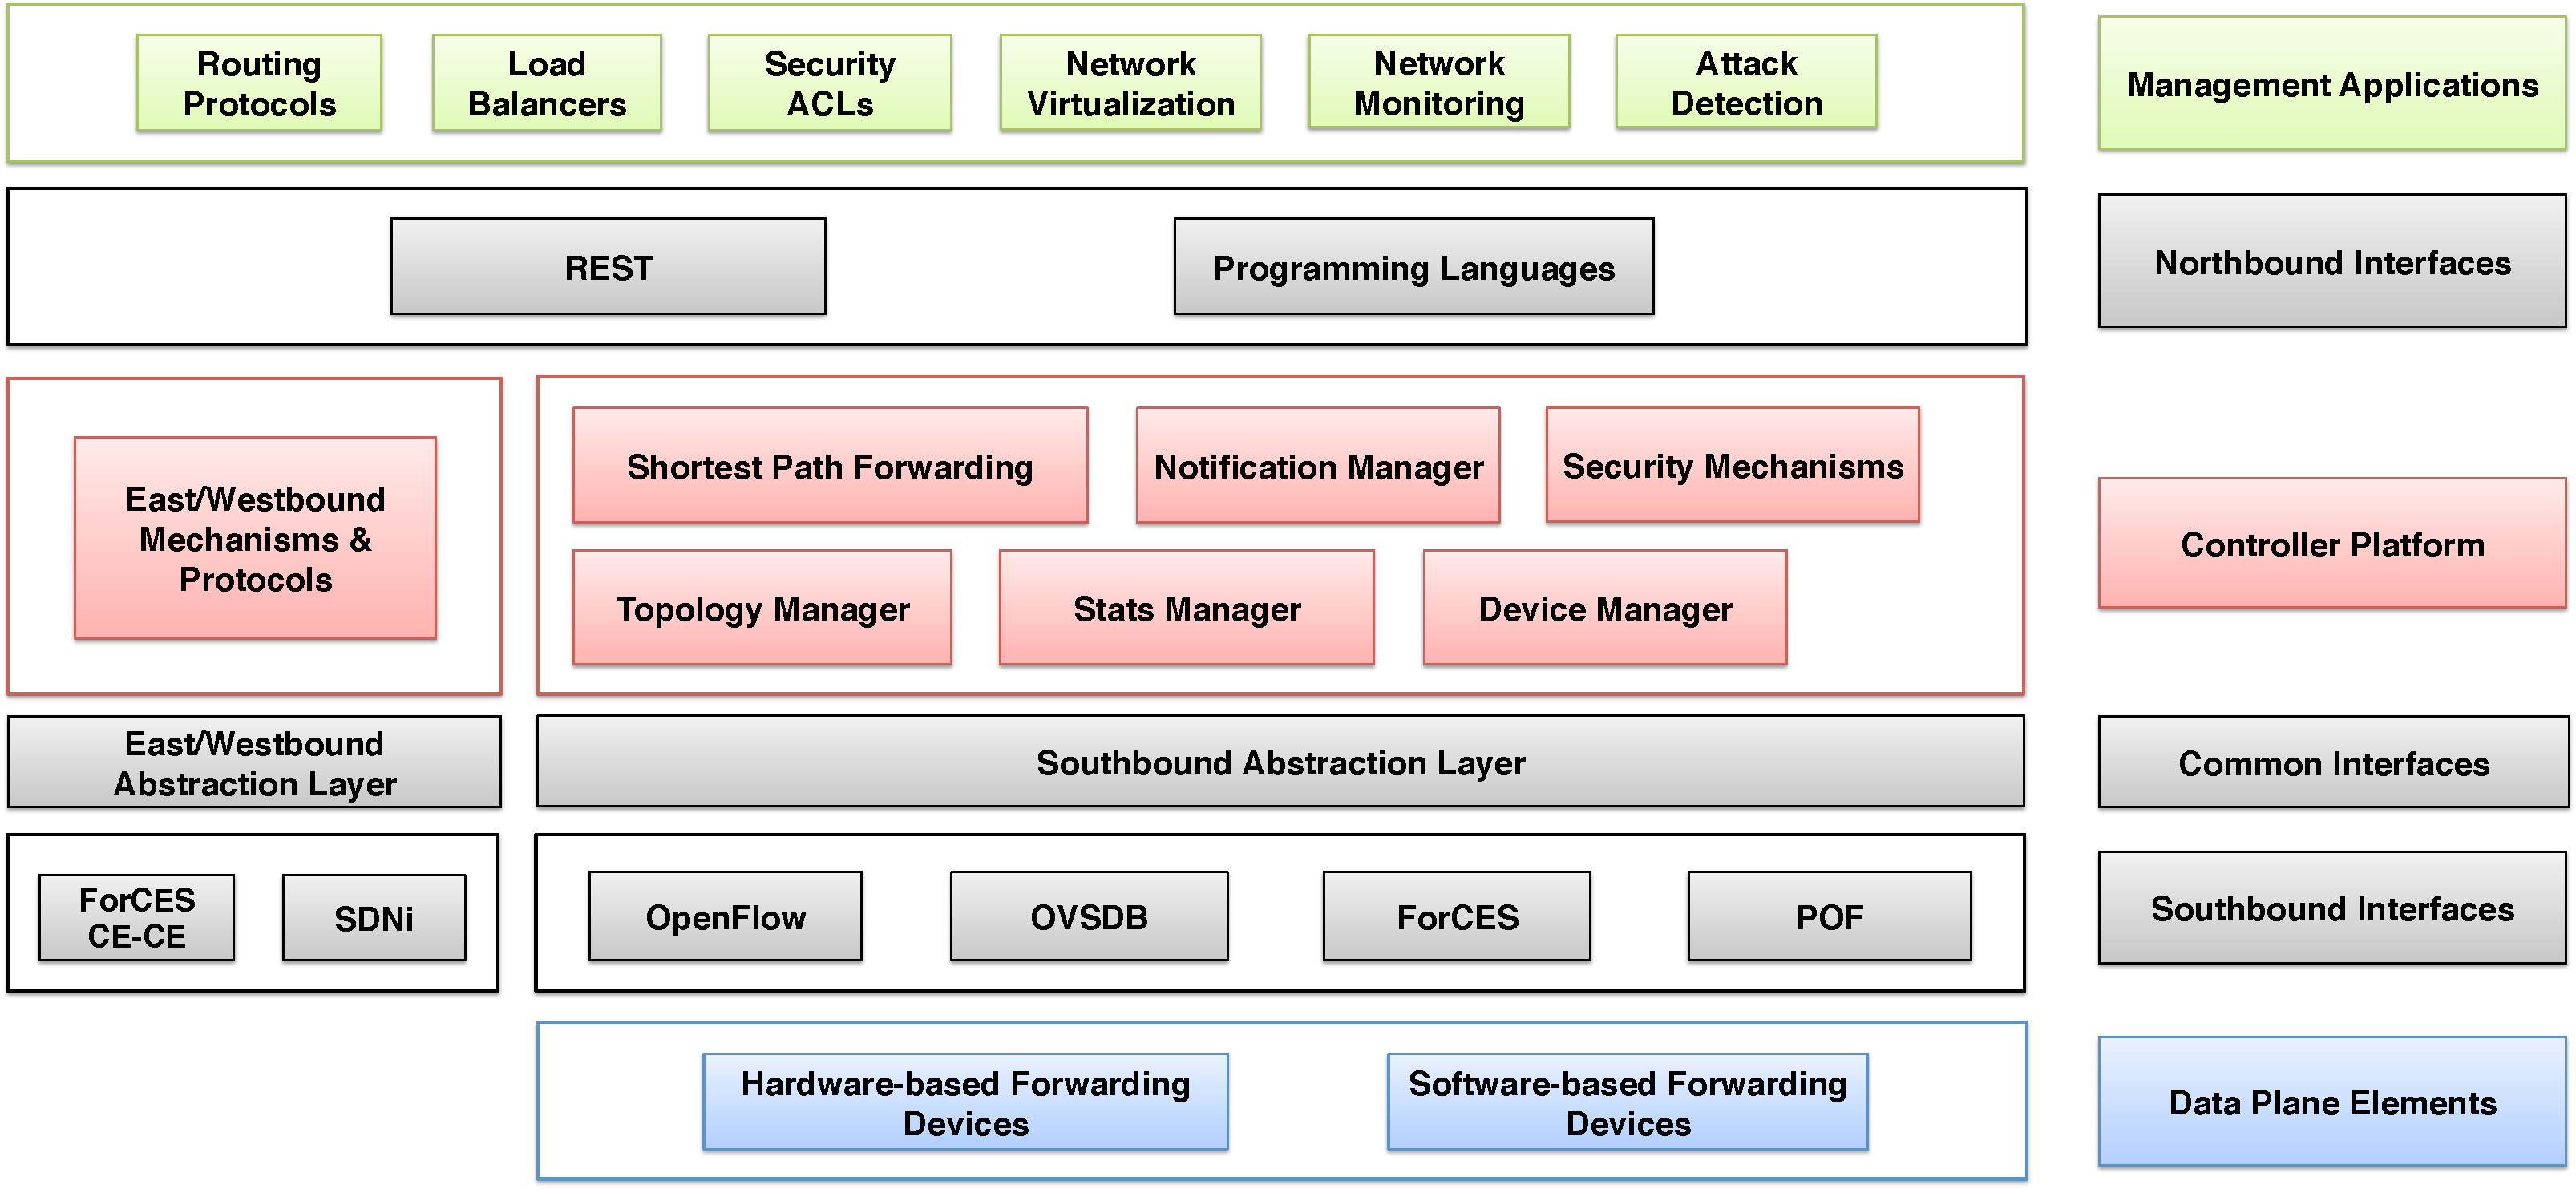
\includegraphics[width=0.85\textwidth]{figures/fig8_sdn_control_platform.pdf}
\caption{SDN control platforms: elements, services and interfaces}
\label{fig:controlplatformarch}
\end{figure*}

There are at least three relatively well-defined layers in most of the existing control platforms: 
(\textit{i}) the application, orchestration and services; (\textit{ii})  the core controller functions, and 
(iii) the elements for southbound communications. The connection at the upper-level layers is based on northbound interfaces such as REST APIs~\cite{richardson2008restful}  and programming languages such as FML~\cite{hinrichs2009}, Frenetic~\cite{foster2011} and NetCore~\cite{monsanto2012}. 
On the lower-level part of a control platform, southbound APIs and protocol plugins interface the forwarding elements. % and the controller platforms. 
The core of a controller platform can be characterized as a combination its base network service functions and the various interfaces. 


\vspace{2mm}
\noindent \textit{Core controller functions}

The base network service functions are what we consider the essential functionality all controllers should provide.
As an analogy, these functions are like base services of operating systems, 
such as program execution, I/O operations control, communications, protection, and so on. 
These services are used by other operating 
system level services and user applications. 
In a similar way, functions such as topology, statistics, notifications and device management, together with shortest path forwarding and security mechanisms are essential network control functionalities that network applications may use in building its logic.
For instance, the notification manager should be able to receive, process, and forward events (e.g., alarm notifications, security alarms, state changes)~\cite{onf2013-2}.
Security mechanisms are another example, as they are critical components to provide basic isolation and security enforcement between services and applications.
For instance, rules generated by high priority services should not be overwritten with rules created by applications with a lower priority.

%On the controller platform, network virtualization services are available for creating and managing 
%virtual tenant networks, traffic redirection services that can be used by routing and security services, 
%distributed overlay virtual Ethernet to deal with scenarios where overlays are required between segments 
%or sites of the network domain, among other specialized functions that may be needed by different services 
%and applications. The number and diversity of specialized services can significantly vary depending on the 
%target deployment scenario. While cloud infrastructure can require cloud integration and virtual tenant 
%network coordinators, these services may not be needed in a common enterprise network deployment.
%Another example could be deployment use cases requiring specialized IP multicasting services~\cite{kotani2012}.
%Therefore, while some services are of common use on most of the SDN deployment and can be considered as 
%essential services of a network operating systems, others are added on-demand accordingly the requirements 
%of the respective target environments.


\vspace{2mm}
\noindent \textit{Southbound}

On the lower-level of control platforms, the southbound APIs can be seen as a layer of device drivers.
They provide a common interface for the upper layers, while allowing a control platform to use different 
southbound APIs (e.g., OpenFlow, OVSDB, ForCES) and protocol plugins to manage existing or new physical or 
virtual devices (e.g., SNMP, BGP, NetConf). This is essential both for backward compatibility and heterogeneity, 
i.e., to allow multiple protocols and device management connectors. Therefore, on the data plane, a mix of physical devices, virtual devices (e.g., Open vSwitch~\cite{listofcontributors2013,pfaff2009}, vRouter~\cite{singla2013}) and a variety of device interfaces (e.g., OpenFlow, OVSDB, of-config~\cite{onf2013-1}, NetConf, and SNMP) can co-exist.

Most controllers support only OpenFlow as a southbound API. Still, a few of them, such as OpenDaylight, 
Onix and HP VAN SDN Controller, offer a wider range of southbound APIs and/or protocol plugins. Onix 
supports both the OpenFlow and OVSDB protocols. The HP VAN SDN Controller has other southbound connectors 
such as L2 and L3 agents. OpenDaylight goes a step beyond by providing a Service Layer Abstraction (SLA) 
that allows several southbound APIs and protocols to co-exist in the control platform. For instance, its 
original architecture was designed to support at least seven different protocols and plugins: OpenFlow, OVSDB~\cite{pfaff2013-1}, NETCONF~\cite{enns2011-1}, PCEP~\cite{vasseur2009}, SNMP~\cite{harrington2002}, BGP~\cite{rekhter2006} and LISP Flow Mapping~\cite{opendaylight2013}. Hence, OpenDaylight is one of 
the few control platforms being conceived to support a broader integration of technologies in a single 
control platform.


\vspace{2mm}
\noindent \textit{Eastbound and Westbound}

East/westbound APIs, as illustrated in Figure~\ref{fig:eastwestbounds}, are a special case of interfaces 
required by distributed controllers.
Currently, each controller implements its own east/westbound API. The functions of these interfaces include
import/export data between controllers, algorithms for data consistency models, and monitoring/notification 
capabilities (e.g., check if a controller is up or notify a take over on a set of forwarding devices).

\begin{figure}[ht]
\centering
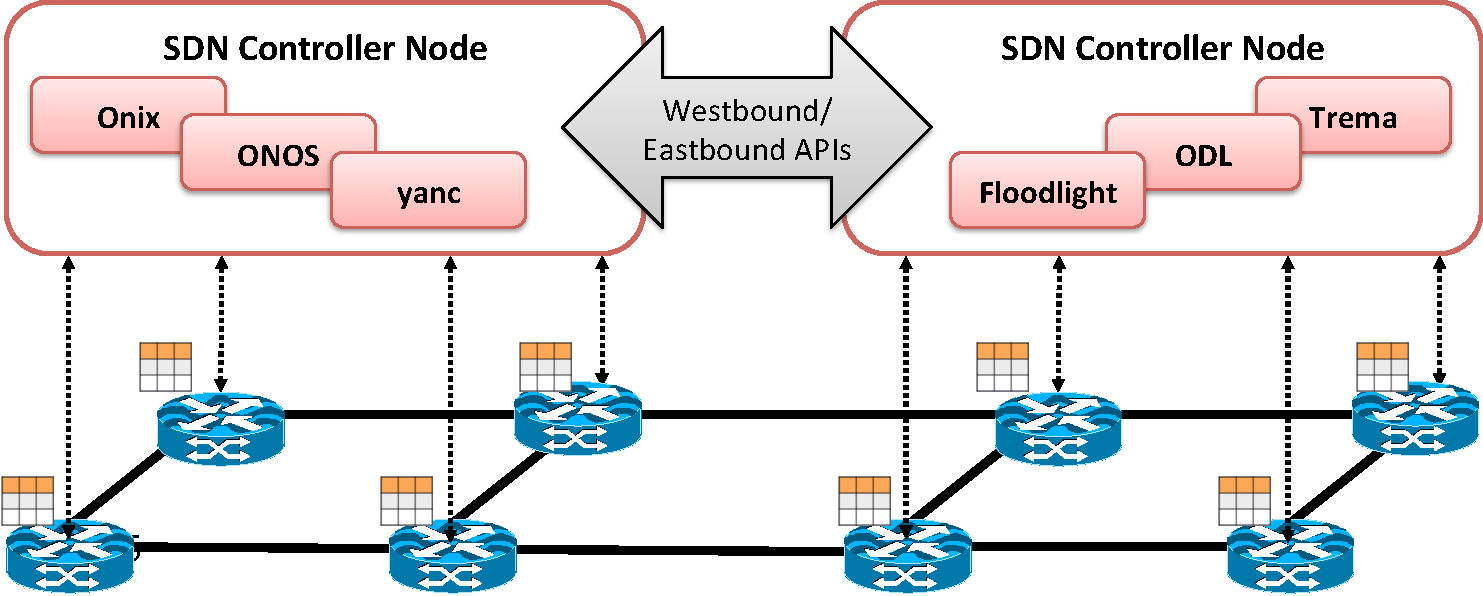
\includegraphics[width=0.99\columnwidth]{figures/fig7_sdn_eastwestbound.pdf}
\caption{Distributed controllers: east/westbound APIs.}
\label{fig:eastwestbounds}
\end{figure}

Similarly to southbound and northbound interfaces, east/westbound APIs are essential components of 
distributed controllers. 
To identify and provide common compatibility and interoperability between 
different controllers, it is necessary to have standard east/westbound interfaces. 
%Examples of early 
%initiatives that propose standard communication protocols and/or mechanisms between distinct control 
%nodes are SDNi~\cite{yin2012}, ForCES CE-CE interface~\cite{doria2010,wang2011-1}, 
%and ForCES Intra-NE mechanisms~\cite{ogawa2013}. 
For instance, SDNi~\cite{yin2012} defines 
common requirements to coordinate flow setup and exchange reachability information across multiple 
domains. 
In essence, such protocols can be used in an orchestrated and interoperable 
way to create more scalable and dependable distributed control platforms. Interoperability can be 
leveraged to increase the diversity of the control platform element. Indeed, diversity increases the 
system robustness by reducing the probability of common faults, such as software faults~\cite{garcia2013}.

%East/westbound APIs are essential building blocks for distributed or clustered controllers.
Other proposals that try to define interfaces between controllers include Onix data import/export functions~\cite{koponen-1}, ForCES CE-CE interface~\cite{doria2010,wang2011-1}, 
ForCES Intra-NE cold-standby mechanisms for high availability~\cite{ogawa2013}, and distributed data stores~\cite{botelho2013}. 
An east/westbound API requires advanced data distribution mechanisms such as the Advanced Message Queuing Protocol  (AMQP)~\cite{vinoski2006} used by
DISCO~\cite{phemius2013}, transactional databases and DHTs~\cite{ghodsi2006} ( as used in Onix~\cite{koponen-1}), or advanced algorithms for strong consistency and fault 
tolerance~\cite{botelho2013}.

In a multi-domain setup, east/westbound APIs may require also more specific communication protocols 
between SDN domain controllers~\cite{stallings2013}. Some of the essential functions of such 
protocols are to \textit{coordinate flow setup} originated by applications, \textit{exchange reachability 
information} to facilitate inter-SDN routing, \textit{reachability update} to keep the network state 
consistent, among others.

\vspace{2mm}
\noindent \textit{Northbound}

%%%NBI
%One of the important components of a network operating systems is the northbound interface.
Current controllers offer a quite broad variety of northbound APIs, such as ad-hoc APIs, RESTful APIs~\cite{richardson2008restful}, 
multi-level programming interfaces, file systems, among other more specialized APIs such as NVP NBAPI~\cite{koponen-1,koponen} and SDMN API~\cite{pentikousis2013}. %\cite{farooq2014}
 Section~\ref{sec:layer-north} is devoted to a more detailed discussion on the evolving layer of northbound APIs.  
 A second kind of northbound interfaces are those stemming out of SDN programming languages such as  
Frenetic~\cite{foster2011}, Nettle~\cite{voellmy2011-1},
NetCore~\cite{monsanto2012}, Procera~\cite{voellmy2012}, 
and Pyretic~\cite{monsanto2013}.  Section~\ref{sec:programminglanguages} gives a more detailed 
overview of the several existing programming languages for SDN.

%Programming languages are powerful northbound interfaces because they provide higher-level abstractions 
%to application developers, i.e., a programmer does not need to deal with low-level messages and events 
%from southbound interfaces (e.g., OpenFlow) that essentially emulate the behavior of a forwarding device.
%Programming languages such as Pyretic offer high-level policy description languages and logical predicates 
%to compose modular and reusable applications. More interestingly, some programming languages provide back-end 
%interfaces to simplify their integration with different network operating systems. For instance, Pyretic 
%requires only standard sockets and a simple OpenFlow client to be ported to different controllers~\cite{reich2013}.


{\renewcommand{\arraystretch}{1.4}
\begin{table*}[!htp]
\caption{Controllers classification}
\label{tab:controllers}
\begin{center}
\footnotesize
%\rowcolors{1}{lightgray}{white}
\begin{tabularx}{\linewidth}{p{2.94cm}Xp{2.29cm}p{1.47cm}p{0.75cm}p{1.35cm}p{2.1cm}p{0.9cm}}
\hline
\textbf{Name} & \textbf{Architecture} & \textbf{Northbound API} & \textbf{Consistency} & \textbf{Faults} & \textbf{License} & \textbf{Prog. language} & \textbf{Version}\\\hline
Beacon~\cite{erickson2013}     & centralized multi-threaded  & ad-hoc API & no & no & GPLv2 & Java & v1.0 \\\hline
DISCO~\cite{phemius2013} & distributed & REST & --- & yes & --- & Java & v1.1\\\hline
Floodlight~\cite{openflowhub.org2012} & centralized multi-threaded  & RESTful API & no & no & Apache & Java & v1.1 \\\hline
HP VAN SDN~\cite{hp2013-1} & distributed & RESTful API & weak & yes & --- & Java & v1.0 \\\hline
HyperFlow~\cite{tootoonchian2010}  & distributed               & --- & weak & yes & --- & C++ & v1.0 \\\hline
Kandoo~\cite{yeganeh2012}     & hierarchically distributed & --- & no & no & --- & C, C++, Python & v1.0 \\\hline
Onix~\cite{koponen-1}       & distributed               & NVP NBAPI   & weak, strong & yes & commercial & Python, C & v1.0 \\\hline
Maestro~\cite{cai2011}    & centralized multi-threaded  & ad-hoc API & no & no & LGPLv2.1 & Java & v1.0 \\\hline
Meridian~\cite{banikazemi2013} & centralized multi-threaded & extensible API layer & no & no & --- & Java & v1.0\\\hline
MobileFlow~\cite{pentikousis2013} & --- & SDMN API & --- & --- & --- & --- & v1.2 \\\hline
MuL~\cite{Saikia:2013:MuL}        & centralized multi-threaded  & multi-level interface & no & no & GPLv2 & C & v1.0 \\\hline
NOX~\cite{gude2008}       & centralized               & ad-hoc API  & no & no & GPLv3 & C++ & v1.0 \\\hline
NOX-MT~\cite{tootoonchian2012}     & centralized multi-threaded  & ad-hoc API & no & no & GPLv3 & C++ & v1.0 \\\hline
NVP Controller~\cite{koponen} & distributed & --- & --- & --- & commercial & --- & --- \\\hline
OpenContrail~\cite{junipernetworks2013-1} & --- & REST API & no & no & Apache 2.0 & Python, C++, Java & v1.0\\\hline
OpenDaylight~\cite{opendaylight2013} & distributed & REST, RESTCONF & weak & no & EPL v1.0 & Java & v1.\{0,3\} \\\hline
ONOS~\cite{krishnaswamy2013} & distributed & RESTful API & weak, strong & yes & --- & Java & v1.0 \\\hline
POX~\cite{mccauley2012}       & centralized               & ad-hoc API  & no & no & GPLv3 & Python & v1.0 \\\hline
ProgrammableFlow \cite{shimonishi2010} & centralized & --- & --- & --- & --- & C & v1.3 \\\hline
Ryu NOS~\cite{nippontelegraphandtelephonecorporation2012} & centralized multi-threaded & ad-hoc API & no & no & Apache 2.0 & Python & v1.\{0,2,3\}\\\hline
SNAC~\cite{appenzeller2011} & centralized & ad-hoc API & no & no & GPL & C++ & v1.0 \\\hline
Trema~\cite{takamiya2012}      & centralized multi-threaded  & ad-hoc API & no & no & GPLv2 & C, Ruby & v1.0 \\\hline
\textit{Unified Controller}~\cite{racherla2014} & --- & REST API & --- & --- & commercial & --- & v1.0 \\\hline
\textit{yanc}~\cite{monaco2013} & distributed & file system & --- & --- & --- & --- & --- \\\hline
\end{tabularx}
\end{center}
\end{table*}
}

\vspace{2mm}
\noindent \textit{Wrapping up remarks and platforms comparison}

Table~\ref{tab:controllers} shows a summary of some of the existing controllers with their respective 
architectures and characteristics.
As can be observed, most controllers are centralized and multi-threaded.
Curiously, the northbound API is very diverse. In particular, five controllers (Onix, Floodlight, MuL, Meridian and SDN Unified Controller) pay a bit more attention to this interface, as a statement
of its importance. Consistency models and fault tolerance are only present in Onix, HyperFlow, HP VAN SDN, 
and ONOS. Lastly, when it comes to the OpenFlow standard as southbound API, only Ryu supports its three 
major versions (v1.0, v1.2 and v1.3).

%A northbound API is an interface between the resources provided by the controller and applications. 
%It can be a programming language, a framework, or a standard set of functions provided by a library that facilitates the developer's life. 
%These APIs can also provide interoperability between different controllers in the sense that one application can be installed and executed on diverse controllers without any modification.
%The east/westbound APIs are more specific building blocks required by clustered or replicated controllers, i.e., they %are essential services of distributed network operating systems.
%These APIs should implement essential functions for data distribution, consistency models, and integrity guarantees, for instance.

%Essential network services represent the crucial and ``always needed'' network functions such as topology manager, device manager, and shortest path routing.
%Therefore, these services should be provided as built-in functions of controllers.

%Yet, the common abstraction layers are design artifacts to enable different east/westbound APIs, southbound APIs and protocol plug-ins to co-exist. 
%Therefore, they can be seen as a higher level common programming abstraction that suppress the details of lower level APIs, protocols and adaptors needed to connect and manage heterogeneous devices and systems.
%Accordingly, they provide standard programming interfaces for upper level frameworks and services such as programming frameworks and applications (e.g., common read and write methods, flow programming abstractions). 
%Underneath this layer a set of drivers and/or plugins can co-exist for integrating different data plane technologies.
%They are known as southbound APIs or connectors, representing protocols and plugins needed to manage diverse technologies such as OpenFlow, OVSDB, NETCONF, BGP, and SNMP.

%Another interesting thing to observe is that SDN domains~\cite{stallings2013} can be used in the context 
%of one or multiple infrastructure domains. Benefits and reasons for using multiple SDN domains include scalability,
%privacy, and incremental deployment. The scaling capability of a single controller node is not infinite, meaning 
%that it can handle only a limited number of devices. Moreover, privacy policies can be required in a per domain basis.
%For instance, carrier-grade network infrastructures and service providers have diverse kinds of customers that need
%different privacy policies.

%Incremental deployment is also a major requirement for infrastructure providers since it is infeasible to change all the legacy systems at once.
%Specially in transport and large-scale networks, incremental deployments of new control platforms and forwarding devices is a must have property.
%Changing routers, fabric, chassis switches, among other devices, is costly and has to pay off for infrastructure and service providers.

%From the security and dependability perspective it is worth emphasizing that most of the existing controllers are essentially monolithic applications~\cite{monaco2013,monsanto2013,foster2011,cai2011,nippontelegraphandtelephonecorporation2012,openflowhub.org2012,voellmy2011-1}, i.e., there is a domain specific programming language and/or a single resulting executable.
%Consequently, bugs in any part of the control platform (controller, application, module, etc.) can lead to severe consequences on the entire system.
%Even distributed controllers such as HyperFlow, Kandoo, and Onix are comprised of a set of monolithic distributed nodes.

%It is also worth mentioning that there are other research initiatives on controllers and control platforms such as clusters of controllers~\cite{yazici2012}, Hybrid Control Plane~\cite{martinez2011} to integrate OpenFlow Ethernet networks with GMPLS based networks, high performance controller for large multi-core architectures~\cite{theyalehaskellgroup2013}, and Distributed Controllers~\cite{macapuna2010} for data center networking.
%The Hybrid Control Plane~\cite{martinez2011} proposes distributed NOX-based controllers that work together through extended GMPLS protocols.
%The main idea is to provide an unified control platform between packet and circuit networks.
%In more specific use cases, distributed autonomous controllers are employed to manage data centers~\cite{macapuna2010}, for instance.
%In this case, the controllers allotting is done in a top of rack (TOR) basis for higher throughput (in a single TOR) and higher availability.

%Other initiatives propose algorithms for building clusters of controllers~\cite{yazici2012}.
%On the core of such solutions is a sort of coordination framework which helps on building and deploying clusters of controllers for environments requiring higher levels of scalability and reliability such as cloud scale data centers.
%Beacon, NOX, and Maestro were already used to prototype and evaluate coordination frameworks~\cite{yazici2012}.
%Experimental results show that a Beacon cluster is capable of achieving a throughput of six million flows per seconds in a modest set of four dual-core machines with low memory footprint and unmanaged gigabit connection.
%Although the throughput is lower that the one reported in ~\cite{erickson2013-1}, in which the experiments took advantage of a cluster with eight extra large computing nodes from Amazon's Elastic Computer Cloud (16 cores, more than 60GB of RAM, and 10Gb network), it increases approximately linearly with the number of nodes in the cluster.

To conclude, it is important to emphasize that the control platform is one of the critical points for 
the success of SDN~\cite{casemore2012-1}.
One of the main issues that needs to be address in this respect is interoperability. 
This is rather interesting, as it was the very first problem that southbound APIs (such as OpenFlow) tried to solve.
For instance, while WiFi and LTE networks~\cite{Kwan2010survey} need specialized control platforms such as MobileFlow~\cite{pentikousis2013} or SoftRAN~\cite{gudipati2013}, 
data center networks have different requirements that can be met with platforms such as Onix~\cite{koponen-1} or OpenDaylight~\cite{opendaylight2013}. 
For this reason, in environments where diversity of networking infrastructures is a reality, coordination and cooperation between different controllers is crucial. 
Standardized APIs for multi-controller and multi-domain deployments are therefore seen as an important step to achieve this goal.

\subsection{Layer V: Northbound Interfaces}
\label{sec:layer-north}

The North- and Southbound interfaces are two key abstractions of the SDN ecosystem. 
The southbound interface has already a widely accepted proposal (OpenFlow), but a common northbound 
interface is still an open issue.
At this moment it may still be a bit too early to define a standard northbound interface, as use-cases are still being worked out~\cite{dix2013}.
Anyway, it is to be expected a common (or a \emph{de facto}) northbound interface to arise as SDN evolves.
An abstraction that would allow network applications not to depend on specific implementations is important to explore the full potential of SDN 

The northbound interface is mostly a software ecosystem, not a hardware one as is the case of the southbound APIs.
In these ecosystems, the implementation is commonly the forefront driver, while standards emerge later and 
are essentially driven by wide adoption~\cite{guis2012}. Nevertheless, an initial and 
minimal standard for northbound interfaces can still play an important role for the future of SDN. 
Discussions about this issue have already begun ~\cite{dix2013,guis2012,salisbury2012-1,ferro2012,casemore2012,pepelnjak2012,johnson2012,little2013-1}, and a common consensus is that northbound APIs are indeed important but that it is indeed too early to define a single standard right now.
The experience from the development of different controllers will certainly be the basis for coming up with a common application level interface.

Open and standard northbound interfaces are crucial to promote application portability and interoperability among the different the control platforms.
A northbound API can be compared to the POSIX standard in operating systems, representing an abstraction that guarantees programming language and controller independence.
NOSIX~\cite{wundsam2012} is one of the first examples of an effort in this direction. It tries to 
define portable low-level (e.g., flow model) application interfaces, making southbound APIs such as OpenFlow 
look like ``device drivers''. However, NOSIX is not exactly a general purpose northbound interface, but 
rather a higher-level abstraction for southbound interfaces. Indeed, it could be part of the common 
abstraction layer in a control platform as the one described in Section~\ref{sec:controllers}.

Existing controllers such as Floodlight, Trema, NOX, Onix, and OpenDaylight propose and define their own northbound 
APIs~\cite{salisbury2012-1,chua2012}.
However, each of them has its own specific definitions.
Programming languages such as Frenetic~\cite{foster2011}, Nettle~\cite{voellmy2011-1}, NetCore~\cite{monsanto2012}, Procera~\cite{voellmy2012} and Pyretic~\cite{reich2013} also abstract the inner details of the controller functions and data plane behavior from the application developers.
Moreover, as we explain in 
Section~\ref{sec:programminglanguages}, programming languages can provide a wide range of powerful 
abstractions and mechanisms such as application composition, transparent data plane fault tolerance, 
and a variety of basic building blocks to ease software module and application development.

SFNet~\cite{yap2010} is another example of a northbound interface. It is a high-level API that 
translates application requirements into lower level service requests. However, SFNet has a limited scope, 
targeting queries to request the congestion state of the network and services such as bandwidth reservation 
and multicast.

Other proposals use different approaches to allow applications to 
interact with controllers. The \textit{yanc} control platform~\cite{monaco2013} explores 
this idea by proposing a general control platform based on Linux and abstractions such as the virtual file 
system (VFS). This approach simplifies the development of SDN applications as programmers are able to use
a traditional concept (files) to communicate with lower level devices and sub-systems.
 
Eventually, it is unlikely that a single northbound interface emerges as the winner, as the requirements for 
different network applications are quite different. APIs for security applications are likely to be different 
from those for routing or financial applications. One possible path of evolution for northbound APIs are 
vertically-oriented proposals, before any type of standardization occurs, a challenge the ONF has started 
to undertake in addition to open-source SDN controller platform developments (e.g., OpenDaylight, Floodlight,
OpenStack). 
%When and if this happens, the NBAPI might become more like an OS API (e.g., POSIX, iOS, Android), 
%to accommodate the potential wide range of applications that want a piece of the network.

\subsection{Layer VI: Language-based Virtualization}
\label{sec:virtualizationslicing}

Two essential characteristics of virtualization solutions are the capability of expressing modularity 
and of allowing different levels of abstractions while still guaranteeing desired properties such as protection.
For instance, virtualization techniques can allow different views of a single physical infrastructure.
As an example, one virtual ``big switch'' could represent a combination of several underlying forwarding devices.
This intrinsically simplifies the task of application developers as they do not need to think about the sequence of switches where forwarding rules have to be installed, but rather see the network as a 
simple ``big switch''.
Such kind of abstraction significantly simplify the development 
and deployment of complex network applications, such as advanced security related services.

Pyretic~\cite{reich2013} is an interesting example of a programming language that offers this type of high-level abstraction of network topology.
It incorporates this concept of abstraction by introducing network objects.
These objects consist of an abstract network topology and the sets of policies applied to it.
Network objects simultaneously hide information and offer the required services.

%An abstract topology can be a single big switch or a set of virtual switches spanned over the physical network.
%This means that Pyretic supports both ``one-to-many'' and ``many-to-one'' mappings, which empowers network 
%programmers with high flexible network topology abstractions for creating modular and composable SDN applications.
%For instance, a typical MAC-learning application is not suitable to learn the location of hosts in large networks.
%However, with topology abstractions, one can deploy the MAC-learning functionality only at the edge of the 
%network, where it is really needed and effective. 
%Beyond that, combine this application with a second one, 
%e.g., shortest-path routing and multicast trees, used to control the core of the network.

Another form of language-based virtualization is static slicing. 
This a scheme where the network is sliced by a compiler, based on application layer definitions.
The output of the compiler is a monolithic control program that has already slicing definitions and configuration commands for the network.
In such a case, there is no need for a hypervisor to dynamically manage the network slices.
Static slicing can be valuable for deployments with specific requirements, in particular those where higher performance and simple isolation guarantees are preferrable to
dynamic slicing.

One example of static slicing approach it the Splendid isolation~\cite{gutz2012}.
In this solution the network slices are made of 3 components:
(a) \textit{topology}, consisting of switches, ports, and links;
(b) \textit{mapping} of slice-level switches, ports and links on the network infrastructure;
(c) \textit{predicates on packets}, where each port of the slice's edge switches has an associated predicate.
The topology is a simple graph of the sliced nodes, ports and links.
Mapping will translate the abstract topology elements into the corresponding physical ones.
The predicates are used to indicate whether a packet is permitted or not to enter a specific slice. 
Different applications can be associated to each slice.
The compiler takes the combination of slices (topology, mapping, and predicates) and respective programs to generate a global configuration for the entire network. 
It also ensures that properties such as isolation are enforced among slices, i.e., no packets of a slice A can traverse to a slice B unless 
explicitly allowed.

Other solutions, such as libNetVirt~\cite{turull2012}, try to integrate heterogeneous technologies for creating 
static network slices. libNetVirt is a library designed to provide a flexible way to create and manage virtual 
networks in different computing environments. Its main idea is similar to the OpenStack Quantum 
project~\cite{quantumcommunicty2012}. While Quantum is designed for OpenStack (cloud environments), 
libNetVirt is a more general purpose library which can be used in different environments. Additionally, 
it goes one step beyond OpenStack Quantum by enabling QoS capabilities in virtual networks~\cite{turull2012}.
The libNetVirt library has two layers: (1) a generic network interface; and (2) technology specific device drivers 
(e.g., VPN, MPLS, OpenFlow). On top of the layers are the management applications and virtual network descriptions.
The OpenFlow driver uses a NOX controller to manage the underlying infrastructure, using OpenFlow rule-based flow 
tables to create isolated virtual networks. By supporting different technologies, it can be used as a bridging 
component in heterogeneous networks.

Table~\ref{tab:virtualizationsolutions} summarizes the hypervisor and non-hypervisor based virtualization 
technologies. 
As can be observed, only libNetVirt supports heterogeneous technologies, not restricting its 
application to OpenFlow-enabled networks. FlowVisor, AutoSlice and OpenVirteX allow multiple controllers, 
one per network slice. FlowN provides a container-based approach where multiple applications from different 
users can co-exist on a single controller. FlowVisor allows QoS provisioning guarantees by using VLAN PCP bits for priority queues.
SDN VE and NVP also provide their own provisioning methods for guaranteeing QoS.

{\renewcommand{\arraystretch}{1.4}
\begin{table*}[!htp]
\caption{Virtualization solutions}
\label{tab:virtualizationsolutions}
\begin{center}
\footnotesize
%\rowcolors{1}{lightgray}{white}
\begin{tabularx}{\textwidth}{p{3cm}p{3.1cm}p{3.1cm}p{2.6cm}X}
\hline
\textbf{Solution} & \textbf{Multiple controllers} & \textbf{Slicing} & \textbf{QoS ``guarantees''} & \textbf{Multi-technology} \\\hline
AutoSlice~\cite{bozakov2012} & yes, one per slice & VLAN tags & no & no, OF only\\\hline
FlowVisor~\cite{sherwood2009,azodolmolky2012} & yes, one per slice & virtual flow tables per slice &  yes (VLAN PCP bits) & no, OF only \\\hline
FlowN~\cite{drutskoy2012,drutskoy2013} & no (contained applications) & VLAN tags  & \textit{unknown} & no, OF only \\\hline
IBM SDN VE~\cite{racherla2014} & yes, a cluster of controllers & logical datapaths & yes (priority-based) & yes (VXLAN, OVS, OpenFlow) \\\hline
libNetVirt~\cite{turull2012} & no, one single controller & VLAN tags & no  & yes (e.g., VPN, MPLS, OpenFlow)\\\hline
NVP's Hypervisor~\cite{koponen} & yes, a cluster of controller & logical datapaths & yes & no, OVS only \\\hline
OpenVirteX~\cite{al-shabibi2014} & yes, one per slice & virtual flow tables per slice & \textit{unknown}  & no, OF only \\\hline 
Pyretic~\cite{reich2013} & no, one single controller & compiler time OF rules & no & no, OF only \\\hline
Splendid Isolation~\cite{gutz2012} & no, one single controller & compiler time VLANs & no  & no, OF only \\
\hline
\end{tabularx}
\end{center}
\end{table*}
}


\subsection{Layer VII: Programming languages}
\label{sec:programminglanguages}

Programming languages have been proliferating for decades. Both academia and industry have evolved 
from low-level hardware-specific machine languages, such as assembly for x86 architectures, to high-level 
and powerful programming languages such as Java and Python. The advancements towards more portable and 
reusable code has driven a significant shift on the computer industry~\cite{guzdial2008,farooq2014}.

Similarly, programmability in networks is starting to move from low level machine languages such as OpenFlow (``assembly'') to high-level programming languages~\cite{foster2011,hinrichs2009,voellmy2011-1,monsanto2012,voellmy2012,monsanto2013,koponen}.
Assembly-like machine languages, such as OpenFlow~\cite{mckeown2008} and POF~\cite{song2013,song2013-1}, essentially mimic the behavior of forwarding devices, forcing developers to spend too much time on low-level details
rather than on the problem solve.
Raw OpenFlow programs have to deal with hardware behavior details such as overlapping rules, the priority ordering of rules, and data-plane inconsistencies that arise from in-flight packets whose flow rules are under installation~\cite{foster2011,monsanto2012,ferguson2012}.
The use of these low-level languages makes it difficult to reuse software, to create modular and extensive code, and leads to a more error-prone development process~\cite{monsanto2013,nelson2014,katta2012}.

Abstractions provided by high level programming languages can significantly help address many 
of the challenges of these lower-level instruction sets~\cite{foster2011,hinrichs2009,voellmy2011-1,monsanto2012,voellmy2012,monsanto2013}.
In SDNs, high-level programming languages can be designed and used to:
\begin{enumerate}
\item create higher level abstractions for simplifying the task of programming forwarding devices;
\item enable more productive and problem-focused environments for network software programmers, speeding up development and innovation;
\item promote software modularization and code reusability in the network control plane;
\item foster the development of network virtualization.
\end{enumerate}

Several challenges can be better addressed by programming languages in SDNs.
For instance, in pure OpenFlow-based SDNs, it is hard to ensure that multiple tasks of a single application 
(e.g., routing, monitoring, access control) do not interfere with each other.
For example, rules generated for one task should not override the functionality of another task~\cite{foster2011,ferguson2012}.
Another example is when multiple applications run on a single controller~\cite{monsanto2013,ferguson2012,porras2012,shin2013-1,son2013}.
Typically, each application generates rules based on its own needs and policies without further knowledge about the rules generated by other applications. As a consequence, conflicting rules can be generated and installed in forwarding devices, which can create problems for network operation.
Programming languages and runtime systems can help to solve these problems that would be otherwise hard to prevent.

Important software design techniques such as code modularity and reusability are very hard to achieve using low-level programming models~\cite{monsanto2013}.
Applications thus built are monolithic and consist of building blocks that can not be reused in other applications.
The end result is a very time consuming and error prone development process.

Another interesting feature that programming language abstractions provide is the capability of 
creating and writing programs for virtual network topologies~\cite{reich2013,gutz2012}.
This concept is similar to object-oriented programming, where objects abstract both data and specific functions 
for application developers, making it easier to focus on solving a particular problem without worrying about 
data structures and their management. For instance, in an SDN context, instead of generating and installing 
rules in each forwarding device, one can think of creating simplified virtual network topologies that represent 
the entire network, or a subset of it. For example, the application developer should be able to abstract the 
network as an atomic big switch, rather than a combination of several underlying physical devices.
The programming languages or runtime systems should be responsible for generating and installing the lower-level 
instructions required at each forwarding device to enforce the user policy across the network. With such kind of 
abstractions, developing a routing application becomes a straightforward process. Similarly, a single physical 
switch could be represented as a set of virtual switches, each of them belonging to a different virtual network.
These two examples of abstract network topologies would be much harder to implement with low-level 
instruction sets. In contrast, a programming language or runtime system can more easily provide abstractions 
for virtual network topologies, as has already been demonstrated by languages such as Pyretic~\cite{reich2013}.

\vspace{2mm}
\noindent \textit{High-level SDN programming languages}


Low-level instruction sets suffer from several problems.
To address some of these challenges, higher-level programming languages have been proposed, with 
diverse goals, such as:
\begin{itemize}
\item Avoiding low-level and device-specific configurations and dependencies spread across the network, as happens
in traditional network configuration approaches; 
\item Providing abstractions that allow different management tasks to be accomplished through easy to understand and maintain network policies;
\item Decoupling of multiple tasks (e.g., routing, access control, traffic engineering);
\item Implementing higher-level programming interfaces to avoid low-level instruction sets;
\item Solving forwarding rules problems, e.g., conflicting or incomplete rules that can prevent a switch event to be triggered, in an automated way;
\item Addressing different race condition issues which are inherent to distributed systems;
\item Enhancing conflict-resolution techniques on environments with distributed decision makers;
\item Provide native fault-tolerance capabilities on data plane path setup;
\item Reducing the latency in the processing of new flows;
\item Easing the creation of stateful applications (e.g., stateful firewall).
\end{itemize}

Programming languages can also provide specialized abstractions to cope with other management requirements, 
such as monitoring~\cite{voellmy2012,foster2011,tootoonchian2010-1}.
For instance, the runtime system of a programming language can do all the ``laundry work'' of installing rules, polling 
the counters, receiving the responses, combining the results as needed, and composing monitoring queries in 
conjunction with other policies. Consequently, application developers can take advantage of the simplicity and 
power of higher level query instructions to easily implement monitoring modules or applications.

Another aspect of paramount importance is the portability of the programming language, necessary so that developers do not 
need to re-implement applications for different control platforms.
The portability of a programming language can be considered as a significant added value to the control plane ecosystem. 
Mechanisms such as decoupled back-ends could be key architectural ingredients to enable platform portability.
Similarly to the Java virtual machine, a portable northbound interface will easily allow applications to run on different controllers without requiring any modification.
As an example, the Pyretic language requires only a standard socket interface and a simple OpenFlow client on the target controller 
platform~\cite{monsanto2013}.

Several programming languages have been proposed for SDNs, as summarized in Table~\ref{tab:programminglanguages}.
The great majority propose abstractions for OpenFlow-enabled networks.
The predominant programming paradigm is the declarative one, with a single exception, Pyretic, which is an imperative language. 
Most declarative languages are functional, while but there are instances of the logic and reactive types.
The purpose -- i.e., the specific problems they intend to solve -- and the expressiveness power vary from language to 
language, while the end goal is almost always the same: to provide higher-level abstractions to facilitate the 
development of network control logic.

{\renewcommand{\arraystretch}{1.4}
\begin{table*}[!htp]
\caption{Programming languages}
\label{tab:programminglanguages}
\begin{center}
\footnotesize
%\rowcolors{1}{lightgray}{white}
\begin{tabularx}{\linewidth}{p{2cm}p{4cm}X}
\hline
\textbf{Name} & \textbf{Programming paradigm} & \textbf{Short description/purpose} \\\hline
FatTire~\cite{reitblatt2013}  & declarative (functional) & Uses regular expressions to allow programmers to describe network paths and respective fault-tolerance requirements. \\\hline
Flog~\cite{katta2012}  & declarative (logic), event-driven & Combines ideas of FML and Frenetic, providing an event-driven and forward-chaining logic programming language. \\\hline
FlowLog~\cite{nelson2014} & declarative (functional) & Provides a finite-state language to allow different analysis, such as model-checking.\\\hline
FML~\cite{hinrichs2009} & declarative (dataflow, reactive) & High level policy description language (e.g., access control).  \\\hline
Frenetic~\cite{foster2011} & declarative (functional) & Language designed to avoid race conditions through well defined high level programming abstractions.  \\\hline
HFT~\cite{ferguson2012}  & declarative (logic, functional) & Enables hierarchical policies description with conflict-resolution operators, well suited for decentralized decision makers. \\\hline
Maple~\cite{voellmy2013} & declarative (functional) & Provides a highly-efficient multi-core scheduler that can scale efficiently to controllers with 40+ cores. \\\hline
Merlin~\cite{soule2013} & declarative (logic) & Provides mechanisms for delegating management of sub-policies to tenants without violating global constraints. \\\hline
nlog~\cite{koponen} & declarative (functional) &  Provides mechanisms for data log queries over a number of tables. Produces immutable tuples for reliable detection and propagation of updates. \\\hline
Nettle~\cite{voellmy2011-1}   & declarative (functional, reactive) & Based on functional reactive programming  principles in order to allow programmers to deal with streams instead of events.   \\\hline
NetCore~\cite{monsanto2012}  & declarative (functional) & High level programming language that provides means for expressing packet-forwarding policies in a high level.  \\\hline
Procera~\cite{voellmy2012}  & declarative (functional, reactive) & Incorporates a set of high level abstractions to make it easier to describe reactive and temporal behaviors.  \\\hline
Pyretic~\cite{monsanto2013}  & imperative & Specifies network policies at a high level of abstraction, offering transparent composition and topology mapping. \\\hline
\end{tabularx}
\end{center}
\end{table*}
}


% FIXME: think about it... this last part can be eventually suppressed
Programming languages such as FML~\cite{hinrichs2009}, 
Nettle~\cite{voellmy2011-1}, and Procera~\cite{voellmy2012}
are functional and reactive.
Policies and applications written in these languages are based on reactive actions triggered by events (e.g., a new host connected to the network, or the current network load).
Such languages allow users to declaratively express different network configuration rules such as access control lists (ACLs), virtual LANs (VLANs), and many others.
Rules are essentially expressed as allow-or-deny policies, which 
are applied to the forwarding elements to ensure the desired network behavior.

Other SDN programming languages such as Frenetic~\cite{foster2011},
Hierarchical Flow Tables (HFT)~\cite{ferguson2012}, NetCore~\cite{monsanto2012}, and
Pyretic~\cite{monsanto2013}, were designed with the simultaneous goal of efficiently expressing packet-forwarding policies and dealing with overlapping rules of different applications, offering advanced operators for parallel and sequential composition of software modules.
To avoid overlapping conflicts, Frenetic disambiguates rules 
with overlapping patterns by assigning different integer priorities, while HFT uses hierarchical policies with 
enhanced conflict-resolution operators.

\textit{See-every-packet} abstractions and race-free semantics also represent interesting features provided 
by programming languages (such as Frenetic~\cite{foster2011}). 
The former ensures that \emph{all} control packets will be available for analysis, sooner or later, while the latter provides the mechanisms for
suppressing unimportant packets. As an example, packets that arise from a network race condition, such as due to a concurrent flow 
rule installation on switches, can be simply discarded by the runtime system.

Advanced operators for parallel and sequential composition help bind (through internal workflow operators) 
the key characteristics of programming languages such as Pyretic~\cite{monsanto2013}. Parallel 
composition makes it possible to operate multiple policies on the same set of packets, while sequential 
composition facilitates the definition of a sequential workflow of policies to be processed on a set of 
packets. Sequential policy processing allows multiple modules (e.g., access control and 
routing) to operate in a cooperative way.
By using sequential composition complex applications can be built out of a combination of different modules (in a similar way as pipes can be used to build sophisticated Unix applications).

Further advanced features are provided by other SDN programming languages.
FatTire~\cite{reitblatt2013} is an example of a declarative language that heavily relies on regular 
expressions to allow programmers to describe network paths with fault-tolerance requirements. For instance, 
each flow can have its own alternative paths for dealing with failure of the primary paths. 
Interestingly, this feature is provided in a very programmer-friendly way, with the application programmer having only to use regular 
expressions with special characters, such as an asterisk. In the particular case of FatTire, an asterisk will produce the same behavior 
as a traditional regular expression, but translated into alternative traversing paths.
%As an example, imagine 
%that a particular flow has to pass through a deep packet inspection middlebox. If in case it can use any path 
%from the ingress switch to the DPI device, a regular expression can be used to declare that the flow is allowed 
%to pass any path (*) leading to the DPI system. Consequently, if the primary path fails, alternative paths will 
%be available and ready to thwart the problem.

Programming languages such as FlowLog~\cite{nelson2014} and Flog~\cite{katta2012} bring 
different features, such as model checking, dynamic verification and stateful middleboxes. For instance, using a programming language such as Flog, it is possible to build a 
stateful firewall application with only five lines of code~\cite{katta2012}.

Merlin~\cite{soule2013} is one of the first examples of unified framework for controlling different network components, such as forwarding devices, middleboxes, and end-hosts.
An important advantage is backward-compatibility with existing systems.
To achieve this goal, Merlin generates specific code for each type of component.
Taking a policy definition as input, Merlin's compiler determines forwarding 
paths, transformation placement, and bandwidth allocation.
The compiled outputs are sets of component-specific 
low-level instructions to be installed in the devices.
Merlin's policy language also allows operators to delegate the control of a sub-network to tenants, while ensuring isolation.
This delegated control is expressed by means of policies that can be further refined 
by each tenant owner, allowing them to customize policies for their particular needs. 
%The verification capability 
%is a natural requirement to avoid that different tenants specialize policies in such a way that it can cause 
%interference on other tenants. To avoid problems among tenants, the verification process has to guarantee 
%isolation, i.e., check whether the extended policy of a tenant is a valid specialization of the original 
%policy and does not violate any isolation requirement. Finally, the framework tries also to distribute 
%enforcement mechanisms (e.g., bandwidth constraints) to end-hosts, reducing the contention in forwarding 
%elements.

Other recent initiatives (e.g., systems programming languages~\cite{casey2013}) 
target problems such as detecting anomalies to improve the security of network protocols (e.g., OpenFlow), 
and optimizing horizontal scalability for achieving high throughput in applications running on multicore 
architectures~\cite{voellmy2013}.
%One of the key ideas behind systems programming languages 
%is to offer support new ways of expressing network protocol message structures and constraints. With a smart 
%enough compiler, these definitions can be used to identity and take countermeasures against known protocol 
%vulnerabilities, for instance.

%One arguable dichotomy of SDN is its reliance on software artefacts expected to yield a high-level defined, 
%flexible yet robust networking paradigm (cf.~\cite{doyle2005}).
Most of the value of SDN will come from the network managements applications built on top of the infrastructure.
Advances in high-level programming languages are a fundamental component to the success of a prolific SDN 
application development ecosystem. To this end, efforts are undergoing to shape forthcoming standard 
interfaces (cf.~\cite{kuzniar2013}) and towards the realization of integrated development 
environments (e.g., NetIDE~\cite{facca2013}) with the goal of fostering the development of a myriad of SDN applications.
We discuss these next.

\subsection{Layer VIII: Management applications}

Management applications can be seen as the ``network brains''. 
They implement the control-logic that will be translated into commands to be installed in the data plane, dictating the behavior of the forwarding devices.
Taking a simple application as routing as an example. 
The logic of this application is to define the path through which packets will flow from 
a point A to a point B.
To achieve this goal a routing application has to, based on the topology input, decide on the path to use and instruct the controller to install the 
respective forwarding rules in all forwarding devices on the chosen path, from A to B.

Software-defined networks can be deployed on any traditional network environment, from home and enterprise networks to data centers and Internet exchange points.
Such variety of environments has led to a wide array of management applications.
Existing network management applications perform traditional functionality such as routing, load balancing, and security policy enforcement, but also explore novel approaches, such as reducing power consumption . 
Other examples include fail-over and reliability functionalities to the data plane, end-to-end QoS enforcement, network virtualization, mobility management in wireless networks, among many others.

%Figure~\ref{fig:controllerplusapps} illustrates a controller with a set of three independent groups of applications.
%The first is a routing layer with two applications, discovery and intradomain routing.
%It receives LLD packets from switches and updates the routing table, which is used by the route flow module to configure paths for new flows.
%In the second group we have the security policy enforcement applications.
%For instance, a new user will have to authenticate as soon as he connects to the network, either wired or wireless.
%Depending on his authorizations, distinct security policies can be applied to flows belonging to the user.
%As a simple example we can consider the case of a visitor that will be isolated in a special network slice, which allows him to only have access to Internet services (e.g., HTTP and HTTPS).
%The third group is a routing and load balancing layer.
%For instance, some services may be directly accessed by any user, while others may require a load balancing policy.
%The second and third groups of applications generate an output consisting of flow rules for the underlying network infrastructure, which are carried out by the controller to the forwarding elements.
%A single flow setup may require the configuration of several switches across the network.
%
%\begin{figure}[ht]
%\centering
%\includegraphics[width=\columnwidth]{figures/sdn-controller-apps-v1.pdf}
%\caption{A controller and applications}
%\label{fig:controllerplusapps}
%\end{figure}

Despite the wide variety of use cases, most SDN applications can be grouped in one of five categories: traffic engineering, mobility and wireless, measurement and monitoring, security and dependability and data center networking.
Table~\ref{tab:managementapplications} summarizes several applications categorized as such, stating their main purpose, controller where it was implemented/evaluated, and southbound API used.

{\renewcommand{\arraystretch}{1.4}
\begin{table*}[!htp]
\caption{Management applications and services}
\label{tab:managementapplications}
\begin{center}
\footnotesize
%\rowcolors{1}{lightgray}{white}
\begin{tabularx}{\linewidth}{p{2cm}p{3.2cm}p{5.1cm}Xp{3.5cm}}
\hline
\textbf{Group} & \textbf{Solution/Application} & \textbf{Main purpose} & \textbf{Controller} & \textbf{Southbound API} \\
\hline
\multirow{12}{*}{\begin{minipage}{2cm}Traffic \\engineering\end{minipage}} 
& ALTO VPN~\cite{scharf2013} & on-demand VPNs & NMS~\cite{stiemerling2014ALTODeployment,alimi2013} & SNMP \\
& Aster*x~\cite{handigol2009}       & load balancing             &  NOX & OpenFlow      \\
& ElasticTree~\cite{heller2010}   & energy aware routing       &  NOX & OpenFlow      \\
& Hedera~\cite{al-fares2010}        & scheduling / optimization  &  --- & OpenFlow  \\
& In-packet Bloom filter~\cite{macapuna2010}        & load balancing  &  NOX & OpenFlow  \\
& OpenQoS~\cite{egilmez2012} & dynamic QoS routing for multimedia apps & Floodlight  & OpenFlow \\
& Plug-n-Serve~\cite{handigol2009-1}  & load balancing             &  NOX & OpenFlow      \\
& QNOX~\cite{jeong2012}          & QoS enforcement                &  NOX & Generalized OpenFlow \\
& QoS framework~\cite{kim2010} & QoS enforcement                &  NOX & OF with QoS extensions \\
& QoSFlow~\cite{ishimori2013} & multiple packet schedulers to improve QoS & --- & OpenFlow\\
& SIMPLE~\cite{qazi2013-1}  & middlebox-specific ``traffic steering'' & Extended POX & OpenFlow  \\
& ViAggre SDN~\cite{skoldstrom2013-1} & divide and spread forwarding tables & NOX & OpenFlow\\
\hline
\multirow{9}{*}{\begin{minipage}{2cm}Mobility \\\& \\Wireless\end{minipage}} 
& CROWD~\cite{ali-ahmad2013} & overlapping of LTE and WLAN cells & --- & OpenFlow \\
& CloudMAC~\cite{vestin2013} & outsourced processing of WLAN MACs & --- & OpenFlow \\
& FAMS~\cite{yamasaki2011} & flexible VLAN system based on OpenFlow & ProgrammableFlow & OpenFlow \\
& MobileFlow~\cite{pentikousis2013} & flow-based model for mobile networks & MobileFlow & SDMN API\\
& Odin~\cite{suresh2012} & smooth hand-off and load balancing & Floodlight & OpenFlow \\
& OpenRAN~\cite{yang2013} & vertical programmability and virtualization & --- & --- \\
& OpenRoads~\cite{yap2010-1} & control of the data path using OpenFlow & FlowVisor & OpenFlow \\
& SoftRAN~\cite{gudipati2013} & load balancing and interference management & --- & Femto API~\cite{smallcellforum2013,Chandrasekhar2008} \\
\hline
\multirow{7}{*}{\begin{minipage}{2cm}Measurement \\\& \\Monitoring\end{minipage}} 
& BISmark~\cite{kim2013} & active and passive measurements & Procera framework & OpenFlow \\
& FleXam~\cite{shirali-shahreza2013} & flexible sampling extension for OpenFlow & --- & --- \\
& FlowSense~\cite{yu2013} & measure link utilization in OF networks & --- & OpenFlow \\
& measurement model~\cite{jose2011} & model for OF switch measurement tasks & --- & OpenFlow \\
& OpenSketch\,\cite{yu2013-1} & separated measurement data plane & OpenSketch & ``OpenSketch sketches'' \\
& OpenTM~\cite{tootoonchian2010-1} & traffic matrix estimation tool & NOX & OpenFlow \\
& PaFloMon\,\cite{argyropoulos2012} & passive monitoring tools defined by users & FlowVisor & OpenFlow \\
\hline
\multirow{15}{*}{\begin{minipage}{2cm}Security \\\& \\Dependability\end{minipage}} 
& Active security~\cite{hand2013} & integrated security using network feedback control & Floodlight & OpenFlow \\
& AVANT-GUARD~\cite{shin2013-3} & DoS security specific extensions to OF & POX & OpenFlow \\
& CloudWatcher~\cite{shin2012}  & framework for monitoring clouds & NOX & OpenFlow      \\
& DDoS detection~\cite{braga2010-1}     & attacks detection and mitigation    &  NOX & OpenFlow      \\
& Elastic IP and Security Group~\cite{stabler2012}  & an SDN based implementation of Amazon's Elastic IP and Security Groups & NOX & OpenFlow   \\
& Ethane~\cite{casado2007-1}   & flow-rule enforcement (match/action)&  Ethane controller & first instance of OpenFlow  \\
& FortNOX ~\cite{porras2012}    & security flow rules prioritization &  NOX & OpenFlow      \\
& FRESCO ~\cite{shin2013-1}    & framework for security services composition & NOX & OpenFlow      \\
& LiveSec~\cite{wang2012-1}       & security policy enforcement          &  NOX & OpenFlow      \\
& NetFuse~\cite{wang2013} & protection against OF traffic overload & --- & OpenFlow \\
& OF-RHM~\cite{jafarian2012}    & random host mutation (defense) &  NOX & OpenFlow      \\
& OpenSAFE~\cite{ballard2010} & direct spanned net traffic in arbitrary ways & NOX & OpenFlow \\
& Reliable multicasting~\cite{kotani2012} & reduce packet loss when failures occur & Trema & OpenFlow \\
& SANE~\cite{casado2006}       & security policy enforcement         &  SANE controller & SANE header (pre-OpenFlow) \\
& VAVE~\cite{yao2011} & source address validation with a global view & NOX & OpenFlow \\
\hline
\multirow{7}{*}{\begin{minipage}{2cm}Data Center \\Networking\end{minipage}} 
& Big Data Apps ~\cite{wang2012} & optimize network utilization & --- & OpenFlow   \\
& CloudNaaS~\cite{benson2011} & networking primitives for cloud applications & NOX &  OpenFlow  \\
& FlowComb~\cite{das2013} & predicts application workloads & NOX & OpenFlow \\
& FlowDiff~\cite{arefin2013} & detects operational problems & FlowVisor & OpenFlow \\
& LIME~\cite{keller2012} & live network migration & Floodlight & OpenFlow      \\
& NetGraph ~\cite{raghavendra2012} & graph queries for network management & --- & OpenFlow, SNMP   \\
& OpenTCP~\cite{ghobadi2013} & dynamic and programmable TCP adaptation & --- & --- \\
\hline
\end{tabularx}
\end{center}
\end{table*}
}

\vspace{2mm}
\noindent \textit{Traffic engineering}

Several traffic engineering applications have been proposed, including 
ElasticTree~\cite{heller2010}, Hedera~\cite{al-fares2010},
OpenFlow-based server load balancing~\cite{wang2011},
Plug-n-Serve~\cite{handigol2009-1} and Aster*x~\cite{handigol2009},
In-packet Bloom filter~\cite{macapuna2010},
SIMPLE~\cite{qazi2013-1}, QNOX~\cite{jeong2012}, QoS framework~\cite{kim2010},
ALTO~\cite{scharf2013}, and ViAggre SDN~\cite{skoldstrom2013-1}.
The main goals of most applications is to engineer traffic with the aim of minimizing power consumption, maximizing aggregate network utilization, providing optimized load balancing, and other generic traffic optimization techniques.

Load balancing was one of the first applications envisioned for SDN/OpenFlow.
Different algorithms and techniques have been proposed for this purpose~\cite{wang2011,handigol2009,handigol2009-1}. 
One particular concern is the scalability of these solutions.
A technique to allow this type of applications to scale is to use wildcard-based rules to perform proactive load balancing~\cite{wang2011}.
Wildcards can be utilized for aggregating clients requests based on the ranges of IP prefixes, for instance, allowing the distribution and directing of large groups of client requests without requiring controller intervention for every new flow
In tandem, operation in reactive mode may still be used when traffic bursts are detected.
The controller application needs to monitor the network traffic and use some sort of 
threshold in the flow counters to redistribute clients among the servers when bottlenecks are likely to happen.

SDN load-balancing also simplifies the placement of network services in the network~\cite{handigol2009-1}.
Every time a new server is installed, the load-balancing service can take the appropriate actions to seamlessly distribute the traffic among the 
available servers, taking into consideration both the network load and the available computing capacity of the respective servers.
This simplifies network management and provides more flexibility to network operators.
% assumes that web services and computing resources are installed in the network in an arbitrary way, as it commonly happens in an university campus.
%It means that operators of these environments do not have a fine-grained control over the load distribution (e.g., placement of servers and current network traffic in all subnets) on the network when new resources need to be installed, for instance.
%Therefore, Aster*x is different from traditional load balancers in the sense that it uses a more global view of the network conditions to apply load balancing policies.
%As an example, we could have two servers A and B both of them with the same processing capacities.
%However, network traffic bottlenecks are more frequent between clients and the server B due to other services running on the same segment of the network.
%Consequently, the incoming traffic should not always be of 50\% for each server.
%Server A, despite having the exact same processing power, can receive more traffic load because its network path is less likely to have bottlenecks.

Existing southbound interfaces can be used for actively monitoring the data plane load.
This information can be leveraged to optimize the energy consumption of the network~\cite{heller2010}. 
By using specialized optimization algorithms and diversified configuration options, it is possible to meet the 
infrastructure goals of latency, performance, and fault tolerance, for instance, while reducing power consumption.
With the use of simple techniques, such as shutting down links and devices intelligently in response to traffic load dynamics, data center operators can save up to 50\% of the network energy in normal traffic 
conditions~\cite{heller2010}. 

One of the important goals of data center networks is to avoid or mitigate the effect of network bottlenecks on the operation of the computing services offered.
Linear bisection bandwidth is a technique that can be adopted for traffic patterns that stress the network by exploring path diversity in a data center 
topology.
Such technique has been proposed in an SDN setting, allowing the maximization of aggregated network utilization with minimal scheduling overhead~\cite{al-fares2010}. 

SDN can also be used to provide a fully automated system for controlling the configuration of routers.
This can be particularly useful in scenarios that apply virtual aggregation~\cite{ballani2009} .
This technique allows network operators to reduce the data replicated on routing tables, which 
is one of the causes of routing tables' growth~\cite{meyer2007}. 
A specialized routing application~\cite{skoldstrom2013-1} can calculate, divide and configure the routing tables of the different routing devices through a southbound API such 
as OpenFlow.

Traffic optimization is another interesting application for large scale service providers, where dynamic scale-out 
is required. For instance, the dynamic and scalable provisioning of VPNs in cloud infrastructures, using protocolols
such as ALTO~\cite{alimi2013}, can be simplified through an SDN-based approach~\cite{scharf2013}.

Other applications that perform routing and traffic engineering include application-aware 
networking for video streaming~\cite{jarschel2013} and improved QoS by employing multiple packet 
schedulers~\cite{ishimori2013} and other techniques~\cite{kim2010,jeong2012,egilmez2012, kumar2013}.

\vspace{2mm}
\noindent \textit{Mobility \& wireless}

The current distributed control plane of wireless networks is suboptimal for managing the limited 
spectrum, allocating radio resources, implementing handover mechanisms, managing interference, and performing efficient load-balancing between cells.
SDN-based approaches represent an opportunity for making it easier to deploy and manage different types of wireless networks, such as WLANs and cellular 
networks~\cite{suresh2012,yap2010-1,ali-ahmad2013,gudipati2013,li2012,jin2013}.
Traditionally hard-to-implement but desired features are indeed becoming a reality with the SDN-based wireless networks. 
These include seamless mobility through efficient hand-overs~\cite{suresh2012,dely2011,li2012}, load balancing~\cite{suresh2012,gudipati2013}, creation of on-demand virtual access points (VAPs)~\cite{suresh2012,vestin2013}, downlink scheduling (e.g., an OpenFlow switch can do a rate shaping or time division) ~\cite{vestin2013}, dynamic spectrum usage~\cite{vestin2013}, enhanced inter-cell 
interference coordination~\cite{vestin2013,li2012}, device to device offloading (i.e., decide in when and how LTE transmissions should be offloaded to users adopting the D2D paradigm~\cite{yang2013d2d})~\cite{ali-ahmad2013}, per client and/or base station resource block allocations (i.e.,  time and frequency slots in LTE/OFDMA networks, which are known as resource blocks)~\cite{gudipati2013,ali-ahmad2013,jin2013}, control and assign 
transmission and power parameters in devices or in a group basis (e.g., algorithms to optimize the transmission and power parameters of
transmission and power parameters of WLAN devices, define and assign transmission power values to each resource block, at each base station, in LTE/OFDMA networks) ~\cite{ali-ahmad2013,gudipati2013}, simplified administration~\cite{suresh2012,yap2010-1,gudipati2013}, easy management of heterogenous network technologies~\cite{yap2010-1,gudipati2013,yap2010-2}, interoperability between different networks~\cite{yap2010-2,jin2013}, shared wireless infrastructures~\cite{yap2010-2}, seamless subscriber mobility and cellular networks~\cite{li2012}, QoS and access control policies made feasible and easier~\cite{li2012,jin2013}, and easy deployment of new applications 
~\cite{suresh2012,gudipati2013,yap2010-2}. 

%The current distributed control plane of wireless networks is suboptimal for managing the limited 
%spectrum, allocating radio resources, implementing handover mechanisms, managing interference, and performing efficient load-balancing between cells.
%SDN-based approaches represent an opportunity for making it easier to deploy and manage different types of wireless networks, such as WLANs and cellular 
%networks~\cite{suresh2012,yap2010-1,ali-ahmad2013,gudipati2013,li2012,jin2013}.
%Traditionally hard-to-implement but desired features are indeed becoming a reality with the SDN-based wireless networks. 
%These include seamless mobility through efficient hand-overs, load balancing, creation of on-demand virtual access points (VAPs), downlink scheduling, dynamic spectrum usage, enhanced inter-cell 
%interference coordination, device to device offloading, per client resource block allocations, assign 
%transmission power values in groups basis, simplified administration, and easy deployment of new applications 
%~\cite{suresh2012,dely2011,vestin2013,yap2010-1,ali-ahmad2013,gudipati2013,yap2010-1,li2012,jin2013}. 

One of the first steps towards realizing these features in wireless networks is to provide programmable and 
flexible stack layers for wireless networks~\cite{bansal2012,gudipati2013}.
One of the first examples is OpenRadio~\cite{bansal2012}, which proposes a software 
abstraction layer for decoupling the wireless protocol definition from the hardware, allowing shared MAC 
layers across different protocols using commodity multi-core platforms. OpenRadio can be seen as the 
``OpenFlow for wireless networks''. Similarly, SoftRAN~\cite{gudipati2013} proposes to rethink 
the radio access layer of current LTE infrastructures. Its main goal is to allow operators to improve and 
optimize algorithms for better hand-overs, fine-grained control of transmit powers, resource block allocation, 
among other management tasks.

Light virtual access points (LVAPs) is another interesting way of improving the management capabilities of 
wireless networks, as proposed by Odin~\cite{suresh2012}. Differently from OpenRadio, 
it works with existing wireless hardware and does not impose any change on IEEE 802.11 standards. An LVAP is 
implemented as a unique BSSID associated with a specific client, which means that there is a one-to-one mapping 
between LVAPs and clients. This empowers infrastructure operators to provide seamless mobility, load balancing 
and hidden terminal mitigation. For instance, when a user moves from one access point (AP) to another, the 
network mobility management application can automatically and proactively act and move the client LVAP from 
AP to the other. In this way, a wireless client will not even notice that it started to use a different AP 
because there is no perceptive hand-off delay, as it would be the case in traditional wireless networks.

%In~\cite{dely2011} the authors propose and demonstrate an OpenFlow based approach to settle the problem of client mobility in a wireless mesh network.
%The main challenge is on handling the fast migration of client addresses between mesh access points.
%An hybrid architecture comprised of two different control planes can help to address this challenge.
%The first control plane is used to manage OpenFlow based forwarding devices, while the second control plane is required to provide a multi-hop IP control connectivity among the mesh of access points.
%In other words, the independent controllers are used to separate and allow simultaneous monitoring and control traffic to flow through the network.
%Furthermore, the OpenFlow controller uses the monitoring information of the second controller to provide mobility and routing optimization to the network.

%SoftRAN's architecture uses a centralized controller to have a global view of the networks and resources, allowing operators to improve and optimize algorithms for better handovers, fine-grained control of transmit powers, resource block allocation, among other management tasks.
%Its decision making is divided in two groups, those that do affect neighboring devices (e.g., transmit powers, handovers) and those that do not affect radio elements (e.g., resource block allocation on the downlink).
%The later case of decisions can be independently done by the radio element once its decision will not affect other elements of the network.
%However, all operations that do affect neighboring devices or the behavior of the network must be done by the controller.
%SoftRAN is also one of the few solutions that do not use OpenFlow.
%Instead, it uses the FemtoAPI as its southbound API, which is an abstraction being proposed as standard interface to encourage innovation and competition between the hardware and software platforms, and application software in carrier networks.

Very dense heterogeneous wireless networks have also been a target for SDN.
These DenseNets have limitations due to constraints 
such as radio access network bottlenecks, control overhead, and high operational costs~\cite{ali-ahmad2013}.
A dynamic two-tier SDN controller hierarchy can be adapted to address some of these constraints~\cite{ali-ahmad2013}. Local controllers can be used to take fast and fine-grained decisions, while regional 
(or ``global'') controllers can have a broader, coarser-grained scope, i.e., that take slower but more 
global decisions.
In such a way, designing a single integrated architecture that encompasses LTE (macro/pico/femto) and WiFi 
cells, while challenging, seems feasible. 
%It would require providing enhanced wireless mechanisms 
%(e.g., scheduling policy control, relay management, subframe synching), dynamic radio and backhaul configuration, 
%and connectivity management across different wireless technologies, in a seamless and integrated way.

\vspace{2mm}
\noindent \textit{Measurement \& monitoring}

Measurement and monitoring solutions can be divided in two classes. First, applications that provide new 
functionality for other networking services. Second, proposals that target to improve features of OpenFlow-based SDNs, 
such as to reduce control plane overload due to the collection of statistics.

An example of the first class of applications is improving the visibility of broadband 
performance~\cite{sundaresan2011,kim2013}. An SDN-based broadband home connection can 
simplify the addition of new functions in measurement systems such as BISmark~\cite{sundaresan2011}, 
allowing the system to react to changing conditions in the home network~\cite{kim2013}. As an example, a home 
gateway can perform reactive traffic shaping considering the current measurement results of the home network.

The second class of solutions typically involve different kinds of sampling and estimation 
techniques to be applied, in order to reduce the burden of the control plane with respect to the collection of data plane statistics.
Different techniques have been applied to achieve this goal, such as stochastic and deterministic packet sampling techniques~\cite{mehdi2011}, traffic matrix estimation~\cite{tootoonchian2010-1}, and fine-grained monitoring of 
wildcard rules~\cite{wette2013}.
Point-to-point traffic matrix estimation, in particular, can help in network design and operational tasks such as load balancing, anomaly detection, capacity planning and 
network provisioning.
With information on the set of active flows in the network, routing information (e.g., from the routing application), flow paths, and flow counters in the switches it is possible to 
construct a traffic matrix using diverse aggregation levels for sources and destinations~\cite{tootoonchian2010-1}.

Other initiatives of this second class propose a stronger decoupling between basic primitives (e.g., matching and counting) and 
heavier traffic analysis functions such as the detection of anomaly conditions attacks~\cite{bianchi2013}.
A stronger separation favors portability and flexibility.
For instance, a functionality to detect abnormal flows should not be constrained by the basic primitives or 
the specific hardware implementation.
Put another way, developers should be empowered with streaming 
abstractions and higher level programming capabilities.

In that vein, some data and control plane abstractions have been specifically designed for measurement purposes.
OpenSketch~\cite{yu2013-1} is a special-purpose southbound API 
designed to provide flexibility for network measurements.
For instance, by allowing multiple measurement tasks to execute concurrently without impairing accuracy.
The internal design of an OpenSketch switch can be thought of as a pipeline with three stages (hashing, classification, and counting). 
Input packets first pass through a hashing function. 
Then, they are classified according to a matching rule.
Finally, the match rule identifies a counting index, which is used to calculate the counter location in the counting stage. While a TCAM with few 
entries is enough for the classification stage, the flexible counters are stored in SRAM.
This makes the OpenSketch's operation efficient (fast matching) and cost-effective (cheaper SRAMs to store counters).

\vspace{2mm}
\noindent \textit{Security \& Dependability}

An already diverse set of security and dependability proposals is emerging in the context of SDNs.
Most take advantage 
of SDN for improving services required to secure systems and networks, such as policy enforcement (e.g., access 
control, firewalling)~\cite{casado2006,wang2012-1,yao2011,stabler2012}, DoS attacks detection and mitigation~\cite{braga2010-1}, random host mutation (stabler2012) (i.e., randomly and frequently mutate the IP addresses of end-hosts to break the attackers' assumption about static IPs, which is the common case)~\cite{jafarian2012}, monitoring of cloud infrastructures for fine-grained security inspections (i.e., automatically analyze and detour suspected traffic to be  further inspected by specialized network security appliances, such as deep packet inspection systems) ~\cite{shin2012}, traffic anomaly detection~\cite{mehdi2011,braga2010-1}, and so forth~\cite{casado2006,wang2012-1,braga2010-1,jafarian2012,shin2012,stabler2012,yao2011,mehdi2011}.
Others address OpenFlow-based networks issues, such as flow rule prioritization, security 
services composition, and protection against traffic overload~\cite{porras2012,shin2013-1,shin2013-3,wang2013}.

There are essentially two approaches, one involves using SDNs to improve network security, and another for improving the 
security of the SDN \emph{itself}. 
The focus has been, thus far, in the latter.

%An already diverse set of security and dependability proposals is emerging in the context of SDNs.
%Most take advantage 
%of SDN for improving services required to secure systems and networks, such as policy enforcement (e.g., access 
%control, firewalling), DoS attacks detection and mitigation, random host mutation, monitoring of cloud 
%infrastructures, traffic anomaly detection, and so forth~\cite{casado2006,wang2012-1,braga2010-1,jafarian2012,shin2012,stabler2012,yao2011,mehdi2011}.
%Others address OpenFlow-based networks issues, such as flow rule prioritization, security 
%services composition, and protection against traffic overload~\cite{porras2012,shin2013-1,shin2013-3,wang2013}.
%
%There are essentially two approaches, one involves using SDNs to improve network security, and another for improving the 
%security of the SDN \emph{itself}. 
%The focus has been, thus far, in the latter.

\noindent \textit{Using SDN to improve the security of current networks}.
Probably the first instance of SDN was an application for security policies enforcement~\cite{casado2006}. 
An SDN allows the enforcement to be done on the first entry point to the network (e.g., the Ethernet switch to which the user is connected to). 
Alternatively, in a hybrid environment, security policy enforcement can be made on a wider network perimeter through programmable devices (without the need to migrate the entire infrastructure to OpenFlow)~\cite{wang2012-1}.
With either application, malicious actions are blocked before entering the critical regions of the network.

SDN has been successfully applied for other purposes, namely for the detection (and reaction) against DDoS flooding attacks~\cite{braga2010-1}, and active security~\cite{hand2013}.
OpenFlow forwarding devices make it easier to collect a variety of information from the network, in a timely 
manner, which is very handy for algorithms specialized in detecting DDoS flooding attacks

The capabilities offered by software-defined networks in increasing the ability to collect statistics data from the network and of allowing applications to actively program the forwarding devices, are powerful for proactive and smart 
security policy enforcement techniques such as Active security~\cite{hand2013}.
This novel security methodology proposes a novel feedback loop to improve the control of defense mechanisms 
of a networked infrastructure, and is centered around five core capabilities: protect, sense, 
adjust, collect, counter.
In this perspective, active security provides a centralized programming interface that simplifies the integration of mechanisms for detecting attacks, by
a) collecting data from different sources (to identify attacks), 
b) converging to a consistent configuration for the security appliances, and 
c) enforcing countermeasures to block or minimize the effect of attacks.

%SANE~\cite{casado2006} and LiveSec~\cite{wang2012-1} are two examples of SDN based solutions to enforce security control in enterprise networks.
%Yet, FortNOX~\cite{porras2012} and FRESCO~\cite{shin2013-1} represent two initiatives, a security kernel and a framework, that start to tackle with security issues of SDN itself, such as differentiate the flow rule priority of applications in controllers and facilitate security services composition.
%
%SANE~\cite{casado2006} 
%was one of the first security control solutions to adopt the pre-SDN concepts.
%Its key idea is to use a centralized controller to manage and enforce security policies in network devices, which is something that helps to reduce the inherent complexity of managing distributed and independent systems in a network such as firewalls, IPS, IDS, proxies, among other security appliances.
%Moreover, the policy enforcement is done on the first entry point (e.g., Ethernet switch where the user is connected to) rather than in different locations in the network.
%Consequently, malicious users and actions are blocked on the first entry point of the network, reducing internal risks by improving the network control and security.

%LiveSec~\cite{wang2012-1} 
%is one generic solution for improving network security.
%It provides an architecture and mechanisms to allow a broader coverage of security policies and services in a scalable and flexible manner.
%LiveSec allows security teams to solve security problems in production networks by leveraging the advantages of a full-mesh security schema (security enforcement points can be easily installed in any point of the network), linear performance increase (security services can be distributed on-demand through the network), and centralized management using a global information base.
%To achieve these goals, it employs the concept of access-switching layer, allowing security policy enforcement elements to be deployed in traditional networks without requiring OpenFlow enabled switches all over the infrastructure.
%This layer resides between users and legacy infrastructure and is comprised of virtual or physical OpenFlow devices managed by the LiveSec controller, which is responsible for applying and controlling security policy enforcement in the network.

\noindent \textit{Improving the security of SDN itself}.
There are already some research efforts on identifying the critical security threats of SDNs and in augmenting its security and dependability~\cite{porras2012,shin2013-1,kreutz2013}.
Early approaches try to apply simple techniques, such as classifying applications and using rule prioritization, to ensure that rules generated by security applications will not be overwritten by 
lower priority applications~\cite{porras2012}. 
Other proposals try to go a step further by providing a framework for developing security-related applications in SDNs~\cite{shin2013-1}.
However, there is still a long way to go in the development of secure and dependable SDN infrastructures~\cite{kreutz2013}.
An in-deep overview of SDN security issues and challenges can be found in Section~\ref{secSecurity}.

\vspace{2mm}
\noindent \textit{Data Center Networking}

%Nowadays, data centers can be considered as the ``heart of IT infrastructures''.
From small enterprises to large scale cloud providers, most of the existing IT systems and services are strongly dependent on highly scalable and efficient data centers.
Yet, these infrastructures still pose significant challenges regarding computing, storage and networking.
Concerning the latter, data centers should be designed and deployed in such a way as to offer
high and flexible cross-section bandwidth and low-latency, 
QoS based on the application requirements,
high levels of resilience,
%nearly error free communication within a physical server patch, 
%self-adjustable transport protocols,
intelligent resource utilization to reduce energy consumption and improve overall efficiency,
agility in provisioning network resources, for example by means of network virtualization and orchestration with computing and storage,
%management flexibility,
and so forth~\cite{Kant20092939,greenberg2008cost,bari2013}.
Not surprisingly, many of these issues remain open due to the complexity and inflexibility of traditional network architectures.

The emergence of software-defined networks has been expected to change the current state of affairs.
Early research efforts have indeed showed that data center networking can significantly benefit from SDN in solving different problems such as live network migration~\cite{keller2012}, improved network management~\cite{keller2012,arefin2013}, eminent failure avoidance~\cite{keller2012,arefin2013}, rapid deployment from development to production networks~\cite{keller2012}, troubleshooting~\cite{keller2012,raghavendra2012}, and optimization of network utilization~\cite{raghavendra2012,wang2012,das2013,arefin2013}.
SDN can also offer networking primitives for cloud applications, solutions to predict network transfers of applications~\cite{wang2012,das2013}, mechanisms for fast reaction to operation problems, network-aware VM placement~\cite{raghavendra2012,benson2011},  QoS support~\cite{raghavendra2012,benson2011}, realtime network monitoring and problem detection~\cite{raghavendra2012,das2013,arefin2013}, security policy enforcement services and mechanisms~\cite{raghavendra2012,benson2011}, and enable programmatic adaptation of transport protocols~\cite{wang2012,ghobadi2013}.

%Data center networking can benefit from SDN in solving problems such as live network migration~\cite{keller2012}, improved network management~\cite{keller2012,arefin2013}, eminent failure avoidance~\cite{keller2012,arefin2013}, rapid deployment from development to production networks~\cite{keller2012}, troubleshooting~\cite{keller2012,raghavendra2012}, and optimization of network utilization~\cite{raghavendra2012,wang2012,das2013,arefin2013}.
%SDN can also offer networking primitives for cloud applications, solutions to predict network transfers of applications~\cite{wang2012,das2013}, mechanisms for fast reaction to operation problems, network-aware VM placement~\cite{raghavendra2012,benson2011},  QoS support~\cite{raghavendra2012,benson2011}, realtime network monitoring and problem detection~\cite{raghavendra2012,das2013,arefin2013}, security policy enforcement services and mechanisms~\cite{raghavendra2012,benson2011}, and enable programmatic adaptation of transport protocols~\cite{wang2012,ghobadi2013}.
%

%SDN can help infrastructure providers to expose more networking primitives to their customers, such as virtual 
%network isolation, custom addressing, quality of service, interposition of middleboxes and placement of virtual 
%desktop cloud applications~\cite{benson2011,calyam2013}. For instance, OpenFlow-like protocols 
%provide the essential means for implementing and deploying dynamic allocation and migration of network slices 
%as well as deploy applications for fast path selection and load balancing between thin-client sites and virtual 
%desktop clouds.
%
%Data center networking can benefit from SDN in solving problems such as live network migration, improved network management, and optimization of network utilization.
%SDN can also offer networking primitives for cloud applications, solutions to predict network transfers of applications, mechanisms for fast reaction to operation problems, and enable programmatic adaptation of transport protocols~\cite{keller2012,raghavendra2012,wang2012,benson2011,das2013,arefin2013,ghobadi2013}.

SDN can help infrastructure providers to expose more networking primitives to their customers, by allowing virtual network isolation, custom addressing, and the placement of middleboxes and virtual desktop cloud applications~\cite{benson2011,calyam2013}. 
To fully explore the potential of virtual networks in clouds, an essential features is virtual network migration. 
Similarly to traditional virtual machine migration, a virtual network may need to be migrated when its virtual machines move from one place to another. Integrating live migration of virtual 
machines and virtual networks is one of the forefront challenges~\cite{keller2012}.
To achieve this goal it is necessary to dynamically reconfigure all affected networking devices (physical or 
virtual).
This as shown to be possible with SDN platforms, such as NVP~\cite{koponen}.

Another potential application of SDN in data centers is in detecting abnormal behaviors of the network 
operation~\cite{arefin2013}. By using different behavioral models and collecting the necessary 
information from elements involved in the operation of a data center (infrastructure, operators, applications), 
it is possible to continuously build signatures for applications by passively capturing control traffic.
Then, the signature history can be used to identify differences in behavior.
Every time a difference is detected, operators can reactively or proactively take corrective measures.
This can help to isolate abnormal components and avoid further damage to the
infrastructure.

\vspace{2mm}
\noindent \textit{Towards SDN App Stores}

As can be observed in Table~\ref{tab:managementapplications}, most SDN applications rely on NOX and OpenFlow.
NOX was the first controller available for general use, making it a natural choice for most use-cases so far.
As indicated by the sheer number of security-related applications, security is probably one of the killer 
applications for SDNs. Curiously, while most use cases rely on OpenFlow, new solutions such as SoftRAN are 
considering different APIs, as is the case of the Femto API~\cite{smallcellforum2013,Chandrasekhar2008}. This diversity of 
applications and APIs will most probably keep growing in SDN.

There are other kinds of management applications that do not easily fit in our taxonomy, such as Avior~\cite{parraga2013}, OESS~\cite{globalnoc2013}, and SDN App Store~\cite{duckett2013,hp2013-2}.
Avior and OESS are graphical interfaces and sets of software tools that make it easier to configure and manage controllers (e.g., Floodlight) and OpenFlow-enabled switches, respectively.
By leveraging their graphical functions it is possible to program OpenFlow enabled devices without coding in a particular programming language.

The SDN App Store~\cite{duckett2013,hp2013-2}, owned by HP, is probably the first SDN 
application market store. Customers using HP's OpenFlow controller have access to the online SDN App Store 
and are able to select applications to be dynamically downloaded and installed in the controller. 
The idea is similar to the Android Market or the Apple Store, making is easier for developers to provide 
new applications and for customers to obtain them.

\subsection{Cross-layer issues}
\label{sec:debuggingandtroubleshooting}

In this section we look at cross-layer problems such as debugging and troubleshooting, testing, verification, simulation and emulation.

\vspace{2mm}
\noindent \textit{Debugging and troubleshooting}

Debugging and troubleshooting have been important subjects in computing infrastructures, 
parallel and distributed systems, embedded systems, and desktop 
applications~\cite{sigelman2010,layman2013,erlingsson2012,tomaselli2013,tan2010,fonseca2007,trivedi2014}. 
The two predominant strategies applied to debug and troubleshoot are runtime debugging 
(e.g., \texttt{gdb}-like tools) and post-mortem analysis (e.g., tracing, replay and visualization).
Despite the constant evolution and the emergence of new techniques to improve debugging and troubleshooting, 
there are still several open avenues and research questions~\cite{layman2013}.

%Debugging and troubleshooting are particular essential for large scale networks~\cite{zeng2014}.
%These networks pose several additional challenges (e.g., scalability, consistency and performance) 
%for automating the process of troubleshooting and debugging, especially when things go wrong. 
%Very large networks need solutions capable of verifying several thousands of nodes and network 
%elements in a short period of time. Ultimately, the goal is to achieve real-time network diagnosis 
%and correction for very large scale networks, which is still a completely open challenge.

Debugging and troubleshooting in networking is at a very primitive stage.
In traditional networks, engineers and developers have 
to use tools such as \texttt{ping}, \texttt{traceroute}, \texttt{tcpdump}, \texttt{nmap}, 
\texttt{netflow}, and SNMP statistics for debugging and troubleshooting.
Debugging a complex 
network with such primitive tools is very hard.
Even when one considers frameworks such as
XTrace~\cite{fonseca2007}, Netreplay~\cite{anand2010} 
and NetCheck~\cite{zhuang2014}, which improve debugging capabilities in networks, it is still difficult 
to troubleshoot networking infrastructures. For instance, these frameworks require a huge effort in terms of 
network instrumentation. The additional complexity introduced 
by different types of devices, technologies and vendor specific components and features make matters worse.
As a consequence, 
these solutions may find it hard to be widely implemented and deployed in current networks.

Software-defined networks' capability of programming the network offers some hope in this respect.
Its software-based control and the use of open standards for control communication can potentially make debug and troubleshoot easier.
The flexibility and 
programmability introduced by SDN is indeed opening new avenues for developing better tools to debug, troubleshoot, 
verify and test networks~\cite{handigol2012-1,wundsam2011,canini2012-1,rotsos2012-1,al-shaer2010,khurshid2012,kuzniar2012,altekar2010,kuzniar2012}.

Early debugging tools for OpenFlow-enabled networks, such as \texttt{ndb}~\cite{handigol2012-1}, OFRewind~\cite{wundsam2011} and NetSight~\cite{handigol2014}, make it easier to discover the source of network problems such as faulty device firmware~\cite{handigol2012-1}, inconsistent or 
non-existing flow rules~\cite{handigol2012-1,wundsam2011}, lack of reachability~\cite{handigol2012-1,wundsam2011}, and faulty routing~\cite{handigol2012-1,wundsam2011}.
Similarly to the well-known \texttt{gdb} software debugger, \texttt{ndb} provides basic debugging 
actions such as \textit{breakpoint}, \textit{watch}, \textit{backtrace}, \textit{single-step}, and 
\textit{continue}. These primitives help application developers to debug networks in a similar way 
to traditional software.
By using \texttt{ndb}'s postcards (i.e., a unique packet identifier composed of a truncated copy of the packet's header, the matching flow entry, the switch, and the output port), for instance, a programmer is able to quickly identify 
and isolate a buggy OpenFlow switch with hardware or software problems. 
If the switch is 
presenting abnormal behavior such as corrupting parts of the packet header, by 
analyzing the problematic flow sequences with a debugging tool one can find (in a matter of few seconds) where 
the packets of a flow are being corrupted, and take the necessary actions to solve the problem.

The OFRewind~\cite{wundsam2011} tool works differently. The idea is to record and 
replay network events, in particular control messages.
These usually account for less than 1\% of the data 
traffic and are responsible for 95\%-99\% of the bugs ~\cite{altekar2010}. 
This tool allows operators to 
perform fine-grained tracing of network behavior, being able to decide which subsets of the network will 
be recorded and, afterwards, select specific parts of the traces to be replayed. These replays provide 
valuable information to find the root cause of the network misbehavior.

Despite the availability of these debugging and verification tools, it is still difficult to answer questions such as: What is happening to my packets that are flowing from point A to point B? What path do they follow? What header modifications do they undergo on the way? 
To answer some of these questions one could recur to the \emph{history} of the packets. A packet's history corresponds 
to the paths it uses to traverse the network, and the header modifications in each hop of the path.
NetSight~\cite{handigol2014} is a platform whose primary goal is to allow applications that use the history of the packets to be built, in order to find out problems in a network.
This platform is composed of three essential elements: (1) NetSight, with its dedicate servers that receive and 
process the postcards for building the packet history, (2) the NetSigh-SwitchAssist, which can be used in 
switches to reduce the processing burden on the dedicated servers, and (3) the NetSight-HostAssist to generate 
and process postcards on end hosts (e.g., in the hypervisor on a virtualized infrastructure).

\texttt{netwatch}~\cite{handigol2014}, \texttt{netshark}~\cite{handigol2014} and \texttt{nprof}~\cite{handigol2014} are three examples of tools built over NetSight.
The first is a live network invariant monitor. 
For instance, an alarm can be trigged every time a packet violates any invariant (e.g., no loops).
The second, \texttt{netshark}, enables users to define and execute filters on the entire history of packets.
With this tool, a network operator can view a complete list of properties of packets at each hop, such as input port, output port, and packet header values.
Finally, \texttt{nprof} can be used to profile sets of network links to provide data for analyzing 
traffic patterns and routing decisions that might be contributing to link load.

\vspace{2mm}
\noindent \textit{Testing and verification}

Verification and testing tools can complement debugging and troubleshooting.
Recent research~\cite{khurshid2012,altekar2010,al-shaer2010,canini2012-1,kuzniar2012,ruchansky2013,zeng2014} 
has shown that verification techniques can be applied to detect and avoid problems in SDN, 
such as forwarding loops and black holes. Verification can be done at different layers (at the controllers, management applications, or network devices).

%Most of the existing testing and verification solutions can be classified in correctness verification 
%through pre-defined properties and constraints~\cite{canini2012-1,kuzniar2012,son2013}, off-line analysis and verification of specific configuration (e.g., rules of the flow tables)~\cite{al-shaer2010}, online checking of network invariants and %policies~\cite{khurshid2012,kazemian2013}, compliance and performance evaluation of devices by measuring capabilities and bottlenecks~\cite{rotsos2012-1}, formal models for identifying unexpected behavior~\cite{ruchansky2013}, and fast %and scalable verification of the correctness of the entire forwarding state in very large networks~\cite{zeng2014}.
%These diverse techniques and methodologies try to detect or avoid different problems such as forwarding loops,  black holes, incorrect installation of flow rules, no FIFO processing, unawareness of echo, no instant OpenFlow response, forgotten %packers, rule overwrite, and device/system bottlenecks.

%NICE~\cite{canini2012-1},
%OFLOPS~\cite{rotsos2012-1},
%FlowChecker~\cite{al-shaer2010},
%VeriFlow~\cite{khurshid2012},
%OFTEN~\cite{kuzniar2012}, 
%FLOVER~\cite{son2013}, and 
%NetPlumber~\cite{kazemian2013}
% are examples of solutions designed for testing and verification purposes, which are indeed important aspects to assure the correct operation of programmable networks.

Tools such as NICE~\cite{canini2012-1} generate sets of diverse streams of packets 
to test as many as possible events, exposing corner cases such as race conditions.
Similarly, OFLOPS~\cite{rotsos2012-1} provides a set of features and functions that allow 
the development and execution of a rich set of tests on OpenFlow-enabled devices. 
Its ultimate 
goal is to measure the processing capacity and bottlenecks of control applications and forwarding devices.
With this tool, users are able to observe and evaluate forwarding table consistency, flow setup latency, 
flow space granularity, packet modification types, and traffic monitoring capabilities (e.g., counters).

FlowChecker~\cite{al-shaer2010}, OFTEN~\cite{kuzniar2012}, and VeriFlow~\cite{khurshid2012} are three examples of tools to verify correctness 
properties violations on the system. While the former two do offline analysis, the latter is capable of 
online checking of network invariants. Verification constraints include security and reachability issues, 
configuration updates on the network, loops, black holes, etc.

Other formal modeling techniques, such as Alloy, can be applied to SDNs to identify unexpected 
behavior~\cite{ruchansky2013}. For instance, a protocol specification can be weak 
when it under-specifies some aspects of the protocol or due to a very specific sequence of events.
In such situations, model checking techniques such as Alloy can help to find and correct unexpected 
behaviors.

One of the challenges in testing and verification is to verify forwarding tables in very large networks to find routing errors, which can cause traffic losses and security breaches, as quickly as possible.
In large scale networks, it is not possible to assume that the network snapshot, at any point, is consistent, 
due to the frequent changes in routing state.
Therefore, solutions such as HSA~\cite{kazemian2012}, Anteater~\cite{mai2011}, NetPlumber~\cite{kazemian2013} and VeriFlow~\cite{khurshid2012} are not suited for this kind of environment.
Another important issue is related on how fast the verification process is done, especially in modern data centers
that have very tight timing requirements. Libra~\cite{zeng2014} represents one of the first attempts to address 
these particular challenges of large scale networks. 
This tool provides the means for capturing stable and consistent 
snapshots of large scale network deployments, while also applying long prefix matching techniques 
to increase the scalability of the system.
By using MapReduce computations, Libra is capable of verifying the correctness of a 
network with up to 10k nodes within one minute.

\vspace{2mm}
\noindent \textit{Simulation and emulation}

Simulation and emulation software is of particular importance for fast prototyping and testing without the need for expensive physical devices.
Mininet~\cite{lantz2010} is the first system that provides a quick and 
easy way to prototype and evaluate SDN protocols and applications.
One of the key properties of Mininet 
is its use of software-based OpenFlow switches in virtualized containers, providing the exact same semantics of hardware-based OpenFlow  switches. This means that controllers or applications developed and tested in the emulated environment can be (in theory) deployed in an OpenFlow-enabled network without any modification. Users can easily emulate an OpenFlow network with hundreds of nodes and dozens of switches by using a single personal computer.
Mininet-HiFi~\cite{handigol2012} is an evolution of Mininet that enhances the container-based (lightweight) 
virtualization with mechanisms to enforce performance isolation, resource provisioning, and accurate monitoring for 
performance fidelity. 
One of the main goals of Mininet-HiFi is to enable repeatable and realistic network experiments.

Mininet CE~\cite{antonenko2013} and SDN Cloud DC~\cite{teixeira2013} are extensions 
to Mininet for enabling large scale simulations. Mininet CE combines groups of Mininet instances into one cluster 
of simulator instances to model global scale networks. SDN Cloud DC enhances Mininet and POX to emulate an SDN-based 
intra-DC network by implementing new software modules such as data center topology discovery and network traffic generation. 

The capability of simulating OpenFlow devices has been added to the popular ns-3 simulator~\cite{ns3project2013}.  
%allow programmers to simulate OpenFlow based networks using Open vSwitch. 
%Applications developed on this kind 
%of simulators can be deployed on physical OpenFlow compliant environments without surprises.
Another example of large scale simulation is \textit{fs-sdn}, which extends the \textit{fs} simulation engine~\cite{sommers2011} by incorporating a controller and switching components with OpenFlow support.
Its main goal is to provide a more realistic and scalable simulation platform as compared to Mininet.
%As an example, \textit{fs-sdn} generates SNMP-like counters byte/packet/flow measurements to improve the 
%accuracy of the simulation.
STS~\cite{ucbsts2013} is a simulator designed to allow developers to specify and apply a variety of test cases, while allowing them to interactively examine the state of the network.

%Mininet~\cite{lantz2010},
%Mininet-HiFi~\cite{handigol2012},
%ns-3~\cite{ns3project2013}, 
%STS~\cite{ucbsts2013},
%ns-3~\cite{ns3project2013}, 
%\textit{fs-sdn}~\cite{gupta2013}, 
%Mininet CE~\cite{antonenko2013}, and 
%SDN Cloud DC~\cite{teixeira2013} 
%are examples of simulation tools conceive or adapted to software-defined networks.


{\renewcommand{\arraystretch}{1.4}
\begin{table*}[!htp]
\caption{Debugging, verification and simulation}
\label{tab:debuggingverification}
\begin{center}
\footnotesize
%\rowcolors{1}{lightgray}{white}
\begin{tabularx}{\linewidth}{p{1.2cm}p{2.5cm}p{3.5cm}X}
\hline
\textbf{Group} & \textbf{Solution} & \textbf{Main purpose} & \textbf{Short description} \\
\hline
\multirow{5}{*}{Debugging} 
& \texttt{ndb}~\cite{handigol2012-1} & \textit{gdb} alike debugging for networks & It provides basic debugging primitives that help developers to debug their networks. \\
& NetSight~\cite{handigol2014} & multi purpose packet history & Allows operators to build flexible debugging, monitoring and profiling applications. \\ 
& OFRewind~\cite{wundsam2011} & tracing and replay & OFRewind allows operators to do a fine-grained tracing of the network behavior. Operators can decide which subsets of the network will be recorded. \\
\hline
\multirow{15}{*}{Verification} 
& Cbench~\cite{sherwood2011} & evaluate OpenFlow controllers & The Cbench framework can be used to emulate OpenFlow switches which are configured to generate workload to the controller.\\
& FLOVER~\cite{son2013} & model checking for security policies & FLOVER provides a provably correct and automatic method for verifying security properties with respect to a set of flow rules committed by an OF controller.\\
& FlowChecker~\cite{al-shaer2010} & flow table configuration verification & A tool used to verify generic properties of global behaviors based on flow tables.  \\
& NetPlumber~\cite{kazemian2013} & real time policy checking & NetPlumber uses a set of policies and invariants to do real time checking. It leverages header space analysis and keeps a dependency graph between rules.\\
& NICE~\cite{canini2012-1} & remove bugs in controllers & Its main goal is to test controller programs without requiring any type of modification or extra work for application programmers. \\
& OFCBenchmark~\cite{jarschel2012} & evaluate OpenFlow controllers & creates independent virtual switches, making is possible to emulate different scenarios. Each switch has its how configuration and statistics.\\
& OFTEN~\cite{kuzniar2012} & catch correctness property violations & A framework designed to check SDN systems, analyzing controller and switch interaction, looking for correctness condition violation. \\
 & OFLOPS~\cite{rotsos2012-1} & evaluate OpenFlow switches & A framework with a rich set of tests for OpenFlow protocol, enabling to measure capabilities of both switch and applications. \\
& VeriFlow~\cite{khurshid2012} & online invariant verification & It provides real time verification capabilities, while the network state is still evolving. \\
\hline
\multirow{12}{*}{Simulation} 
& \textit{fs-sdn}~\cite{gupta2013} & fast simulation & Like Mininet, it provides a simulation environment, but with speed and scalability advantages.\\
& Mininet~\cite{lantz2010} & fast prototyping & It emulates and OpenFlow network using Open vSwitches to provide the exact same semantics of hardware devices. \\
& Mininet CE~\cite{antonenko2013} & global network modeling & It is a combination of tools to create a Mininet cluster for large scale simulation of network topologies and architectures.\\
& Mininet-HiFi~\cite{handigol2012} & fast prototyping for reproducibility & An evolution of Mininet to enable repeatable and high fidelity network experiments. \\
& ns-3~\cite{ns3project2013} & network simulation & The latest version of ns-3 simulator provides support to OpenFlow, enabling to create programmable network devices. \\
& SDN Cloud DC~\cite{teixeira2013} & cloud data center emulation & The SDN Cloud DC solution allows users to evaluate the performance of their controllers at scale.\\
& STS~\cite{ucbsts2013} & troubleshooting & It simulates a network, allows to generate tricky test cases, and allows interactively examine the state of the network.\\
\hline
\end{tabularx}
\end{center}
\end{table*}
}

\section{Ongoing Research Efforts and Challenges}
\label{sec:challenges}

The research efforts we have surveyed so far seek to overcome the challenges of realizing the vision and fulfilling the potential of SDN.
While Section~\ref{sec:layeredapproach} provided a perspective structured across the layers of the ``SDN stack'', this
section highlights research we consider of particular importance for unleashing the full potential of SDN, and that therefore deserves a specific coverage in this survey.


\begin{comment}

Scalability, security and dependability, organizational barriers,
migration, minimally standardized northbound APIs, and global-scale
network services can be considered as some of the main challenges of
SDNs.  Despite  several works that address different scaling
issues in software-defined networks, scalability still needs attention
in large-scale enterprise
deployments~\cite{yeganeh2013,Li:2012:Toward:0001,yu2010-1}.  For
instance, one of the fundamental demanding features of distributed
network operating systems is consistent data distribution and fault
tolerance.  In control platforms designs the performance penalty for
strong data consistency among controller nodes is significantly
high~\cite{koponen-1}.
%However, recent research have shown that high performance of fault tolerant and strongly consistent data stores for distributed SDN control platforms is an achievable goal~\cite{botelho2013}.
Furthermore, cellular networks, first class data centers and
backbones, are three examples of challenging large-scale  scenarios for SDNs.

Security and dependability are first class priorities of any network architecture, and especially critical for control split approaches as in SDN.
In particular, enterprise deployments demand higher levels of security
and dependability, in order to give the appropriate confidence guarantees to infrastructure stakeholders~\cite{sorensen2012,kerner2013}.
In fact, currently available SDN standards and solutions provide only a few basic  features and properties with respect to security and dependability, such as encrypted TLS channels, flow rate limits, and master/slave controllers to tolerate failures.
However, as will be shown in the following sections, this is far from enough to mitigate most of the existing threats.

Examples of challenges regarding organizational barriers, migration, minimally standardized northbound APIs, and global-scale network services will also be explored throughout the section.
For instance, differently from storage and computing resources, which are nearly globally available through cloud providers, infrastructures that provide flexible Network-as-a-Service are still far from reality.
Despite the fact that SDN brings new means and opportunities, there is a long path to go and many difficulties to overcome, such as how to create cross domain virtual networks with quality of service and quality of protection guarantees.

\end{comment}

%IMplementation challenges:
%http://ieeexplore.ieee.org/xpl/articleDetails.jsp?arnumber=6553676

\subsection{Switch Designs}

% ~\cite{rotsos2012-1,wundsam2012,huang2013}
Currently available OpenFlow switches are very diverse and exhibit notable differences in terms of 
feature set (e.g., flow table size,  optional actions), performance (e.g., fast vs. slow 
path, control channel latency/throughput), interpretation and adherence to the protocol 
specification (e.g., \texttt{BARRIER} command), and architecture (e.g., hardware vs. software designs).

%\subsubsection{Heterogenous Implementations}
\vspace{2mm}
\noindent \textit{Heterogenous Implementations}

Implementation choices have a fundamental impact on the behavior, accuracy, and performance of switches, 
ranging from differences in flow counter behavior~\cite{curtis2011} to a number of 
other performance metrics~\cite{rotsos2012-1}. One approach to accommodate such heterogeneity 
is through NOSIX, a portable API that separates the application expectations from the switch heterogeneity~\cite{wundsam2012}. To do so, NOSIX provides a pipeline of multiple virtual flow 
tables and switch drivers. Virtual flow tables are intended to meet the expectations of applications and 
are ultimately translated by the drivers into actual switch flow tables. 
Towards taming the  complexity of multiple OpenFlow protocol versions with different sets of required and optional capabilities -- a roadblock for SDN practitioners --, tinyNBI~\cite{casey2014} has been proposed as a  simple API providing a unifying set of core abstractions of five OpenFlow protocol versions (from 1.0 to 1.4).
Ongoing efforts to introduce a new Hardware Abstraction Layer  (HAL) for non-OpenFlow capable devices~\cite{alienfp7}  include the development of open source artifacts like ROFL (Revised OpenFlow Library) and the xDPd (eXtensible DataPath daemon), a framework for creating new OpenFlow datapath implementations based on a diverse set of hardware and software platforms.
A related open source effort to develop a common library to implement OpenFlow 1.0 and 1.3 protocol endpoints (switch agents and controllers) is libfluid~\cite{libfluid}, winner of the OpenFlow driver competition organized by the ONF.

Within the ONF, the Forwarding Abstraction Working Group (FAWG) is pursuing another solution to the heterogenity problem, through Table Type Patterns 
(TTPs)~\cite{onf2013}. A TTP is a standards-based and negotiated switch-level behavioral abstraction. 
It consists of the relationships between tables forming a graph structure, the types of tables in the graph, 
a set of the parameterized table properties for each table in the graph, the legal \texttt{flow-mod} and \texttt{table-mod} commands for 
each flow table, and the metadata mask that can be passed between each table pair in the graph. 


%\subsubsection{Flow Table Capacity}
\vspace{2mm}
\noindent \textit{Flow Table Capacity}

Flow matching rules are stored in flow tables inside network devices.
One practical challenge is to provide switches with large and efficient flow tables to store the 
rules~\cite{appelman2012}. TCAMs are a common choice to hold flow tables. While flexible 
and efficient in terms of matching capabilities, TCAMs are costly and usually small (from 4K to 32K 
entries). Some TCAM chips today integrate 18 M-bit (configured as 500k entries $*$ 36 bit per entry) 
into a single chip working at 133 Mhz~\cite{kannan2013}, i.e., capable of 133M lookups 
per second. However, these chips are expensive and have a high-power consumption~\cite{liao2012}, 
representing a major power drain in a switching device~\cite{agrawal2006}. These are some of the reasons 
why currently available OpenFlow devices have TCAMs with roughly 8K entries, where the actual capacity 
in terms of OpenFlow table size has a non-trivial relationship to the type of flow entries being used~\cite{owens2013,salisbury2012}. OpenFlow version 1.1 introduced multiple tables, 
thereby adding extra flexibility and scalability. Indeed, OpenFlow 1.0 implied state explosion due to 
its flat table model~\cite{onf2013}. However, supporting multiple tables in hardware is challenging 
and limited -- yet another motivation for the ongoing ONF FAWG work on TTPs~\cite{onf2013}.

%\subsubsection{Performance}
\vspace{2mm}
\noindent \textit{Performance}

 Commercial OpenFlow switches today support only around 200 control events (e.g., 
\texttt{packet-in}, \texttt{flow-mod}) per second~\cite{stephens2012-1}. This is clearly a limiting 
factor that shall be addressed in the switch design process -- support of OpenFlow in existing product 
lines has been more a retrofitting activity than a clean feature planning and implementation activity. Deployment experiences~\cite{Kobayashi2014151} have pointed to a series of challenges stemming from the limited embedded CPU power of current commercial OpenFlow switches. 
One approach to handle the problem consists of adding more powerful CPUs into the switches, as proposed 
in~\cite{mogul2012}. Others have proposed to rethink the distribution of control 
actions between external controllers and the OpenFlow agent inside the switch~\cite{curtis2011}. 
Our current understanding indicates that an effective way forward is a native design of SDN switches 
consistent with the evolution of the southbound API standardization activities~\cite{bosshart2013-1,onf2013}. 

% Note: NetVM~\cite{hwang2014} is an approach for high performance, line rate, within new technologies such as DPDK~\cite{intelcorporation2014}.

%\subsubsection{Evolving Switch Designs}
\vspace{2mm}
\noindent \textit{Evolving Switch Designs}

New SDN switch designs are expected to appear in a myriad of hardware 
combinations to efficiently work together with TCAMs, such as SRAM, RLDRAM, DRAM, GPU, FPGA, NPs, CPUs, 
among other specialized network processors~\cite{ferkouss2011,naous2008,memon2013,luo2009,rostami2012,pongracz2013}. These early works suggest the need for additional efforts into new hardware architectures for future 
SDN switching devices. For instance, some proposals target technologies such as GPUs that have demonstrated 
20 Gbps with flow tables of up to 1M exact match entries and up to 1K wildcard entries~\cite{memon2013}. 
Alternatives to TCAM-based designs include new hardware architectures and components, as well as new and more 
scalable forwarding planes, such as the one proposed by the Rain Man firmware~\cite{stephens2012}.
Other design solutions, such as parallel lookup models~\cite{li2013}, can also be applied to SDN to reduce 
costs in switching and routing devices. Recent proposals on cache-like OpenFlow switch arrangements~\cite{katta2013} shed some light on overcoming the practical limitations of 
flow table sizes with clever switching designs. Additionally, counters represent another practical challenge 
in SDN hardware implementations. Many counters already exists, and they could lead to significant control 
plane monitoring overhead~\cite{curtis2011}. Software-defined counters 
(SDC)~\cite{mogul2012} have been proposed to provide both scalability and flexibility.

%\subsubsection{Hardware Enhancements/Support}
\vspace{2mm}
\noindent \textit{Hardware Enhancements \& Support}

As in any soft\-wa\-re/hard\-wa\-re innovation cycle, a number of advancements can be expected from the hardware 
perspective to improve SDN capabilities and performance~\cite{intelprocessors2012,brebner2012,appelman2012,matsumoto2012,naous2008,bianco2010}.
Microchip companies such as Intel are already shipping processors with flexible SDN capabilities to the 
market~\cite{intelprocessors2012}. Recent advances in Intel general-purpose CPU technology include a 
data-plane development kit~(DPDK)~\cite{intelcorporation2014} that allows high-level programming of how data 
packets shall be processed directly within network interface cards. Prototype implementations of an Intel 
DPDK accelerated switch shows the potential to deliver high-performance SDN software switches without 
giving up the flexibility of programmable data planes~\cite{pongracz2013}. This trend is likely to 
continue since high-speed and specialized hardware is needed to boost SDN performance and scalability for 
large, real-world networks. Hardware-programmable technologies such as FPGA are widely used to reduce time 
and costs of hardware-based feature implementations. NetFPGA, for instance, has been a pioneering technology 
used to implement OpenFlow 1.0 switches~\cite{naous2008}, providing a commodity 
cost-effective prototyping solution. Another line of work on SDN data planes proposes to augment switches 
with FPGA to (remotely) define the queue management and scheduling behaviour of packet 
switches~\cite{sivaraman2013}.

%\subsubsection{Native SDN Switch Designs}
\vspace{2mm}
\noindent \textit{Native SDN Switch Designs}

Most of the SDN switch (re)design efforts so far follow an evolutionary approach, to retrofit 
OpenFlow-specific programmable features into existing hardware layouts, following common wisdom 
on switch/router designs and consolidated technologies (e.g., SRAM, TCAM). One departure from 
this approach is the ongoing work on \textit{forwarding metamorphosis}~\cite{bosshart2013-1}, 
a reconfigurable match table model inspired from RISC-like pipelined architecture applied to switching 
chips. This work illustrates the feasibility of realizing a minimal set of action primitives for flexible 
header processing in hardware, at almost no additional cost or power. Also in line with the core SDN goals 
of highly flexible and programmable (hardware-based) dataplanes, Protocol-Oblivious Forwarding (POF)~\cite{song2013-1} aims at overcoming some of the limitations of OpenFlow (e.g., expressiveness, 
support of user-defined protocols, memory efficiency), through generic flow instruction sets.
Open-source prototypes are available~\cite{song2013} as well as evaluation 
results showing the line-speed capabilities using a network processing unit (NPU)-based~\cite{Hauger2009} proof of 
concept implementation. 


Pretty much as TTPs allow controllers to compile the right set of low-lever instructions known to be supported by the switches, a new breed of switch referred to as P4 (programmable, protocol-independent packet
processor)~\cite{bosshart2013} suggests an evolution path for OpenFlow, based on a high-level compiler. 
 The proposed flexibility would allow the functionality of programmable switches (i.e., pipeline, header parsing, field matching) to be not only specified by the controller but also changed in the field. In this model, 
programmers are able to decide how the forwarding plane processes packets without caring about implementation details due to  a compiler that transforms an imperative program into a control flow graph that can be mapped to different specific target switches. 



% http://conferences.sigcomm.org/sigcomm/2013/papers/hotsdn/p127.pdf

% Fast Programmable Match-Action Processing in Hardware for SDN
%On the cost and speed:
%\begin{itemize}
%\item Single Match Table: costly and wastful
%\item Multiple Match Tables: severely limits flexibility and limited repertoire of actions corresponding to common processing behaviors
%\item Reconfigurable Match Tables: allows a set of pipeline stages and four ways of data plane reconfigurability
%\end{itemize}


%OpenPipes: Prototyping high-speed networking systems~\cite{gibb2009}
%Build and connect high performance modules via OpenFlow network...

%
%ServerSwitch: A Programmable and High Performance Platform for Data Center Networks~\cite{lu2011}
%
%Stochastic Switching Using OpenFlow~\cite{shourmasti2013}
%
%ITEM hardware architectures, devices and performance ... ~\cite{intelprocessors2012,brebner2012,appelman2012,matsumoto2012,naous2008,bianco2010}
%
%ITEM Switch implementation and performance issues... ~\cite{rotsos2012-1,bianco2010,curtis2011,yu2010-1};
%
%There are several challenges related to the forwarding plane performance~\cite{rotsos2012-1,bianco2010,curtis2011,yu2010-1}.
%
%
%
%Towards TCAM-based Scalable Virtual Routers~\cite{luo2012}
%
%
%Accelerating OpenFlow Switching with Network Processors~\cite{luo2009}
%
%A 100Gig network processor platform for openflow~\cite{ferkouss2011}
%
%FlashFlow: a GPU-based Fully Programmable OpenFlow Switch~\cite{memon2013}
%Goal: reach 20 Gbps with flow tables of up to 1M exact match entries and up to 1K wildcard entries.
%
%\note{DK ... 
%    In some earlier work ~\cite{das2011-1}, authors apply network processor based acceleration cards to perform OpenFlow switching. They propose and describe the design options and report re- sults that show a 20\% reduction on packet delay. Also, in ~\cite{Yap:2010:TSN:1851276.1851288}, an architectural design to improve look-up performance of OpenFlow switching in Linux is proposed. Preliminary results reported show a packet switching throughput increase up to 25\% compared to the throughput of regular software-based OpenFlow switching. Another study on dataplane performance over Linux based OpenFlow switching is presented in ~\cite{foster2011}.
%}


\subsection{Controller Platforms}

In the SDN model, the controller platform is a critical pillar of the architecture, and, as such, 
efforts are being devoted to turn SDN controllers into high-performance, scalable, distributed, 
modular, and high-available pieces of programming-friendly software.

%\begin{itemize}
%\item Distribution:
%\item Elasticity:
%\item Architecture:
%\item Orchestration:
%\item Modularity:
%\end{itemize}

%

\vspace{2mm}
\noindent \textit{Performance}

As the SDN community learns from the development and operational experiences with OpenFlow controllers (e.g., Beacon~\cite{erickson2013-1}), further advancements are expected in terms of raw performance of controller implementations~\cite{azodolmolky2013-2}, including the exploitation of hierarchical designs and optimized buffer sizing~\cite{azodolmolky2013-2}. A more detailed discussion on performance evaluation will be presented in Section~\ref{sec:performance-eval}. 
%While the first commercially available controllers supporting OpenFlow 1.3 are capable of handling up to 200 physical switches per controller and/or 10.000 ports~\cite{little2013}, we expect these numbers to be transient

%Performance Evaluation of a Scalable Software-Defined Networking Deployment
%Given these parameters, the required buffer size of the root SDN controller amounts to 0.83 million events in worst case scenario. This result helps the designers provision the required buffer space (i.e., buffer sizing

% Modularity
%\subsubsection{Modularity}
\vspace{2mm}
\noindent \textit{Modularity}

As in software engineering in general, lack of modularity results in controller 
implementations that are hard to build, maintain, and extend -- and ultimately become resistant to further 
innovations, resembling traditional ``hardware-defined'' networks. As surveyed in Section~\ref{sec:programminglanguages}, 
SDN programming abstractions (e.g.,~Pyretic~\cite{monsanto2013}) introduce modularity in SDN 
applications and simplify their development altogether. Further research efforts (e.g., 
Corybantic~\cite{auyoung2013}) try to achieve modularity in SDN control programs. Other 
contributions towards achieving modular controllers can be expected from other areas of computer science 
(e.g., principles from Operating System~\cite{monaco2013}) and best practices of modern 
cloud-scale software applications.

%\subsubsection{High Availability}
% Production quality, HA
\vspace{2mm}
\noindent \textit{High Availability}

In production, SDN controllers need to sustain healthy operation 
under the pressure of different objectives from the applications they
host. Many advances are called for in order
to deal with potential risk vectors of controller-based solutions~\cite{kreutz2013}. Certainly, 
many solutions will leverage on results from the distributed systems and security communities made over the last decade. 
Recent efforts are evolving towards consistent, fault-tolerant data stores~\cite{botelho2013}. 

%%% autoscaling paper

%\subsection{Data Plane Performance}
%
%NetVM~\cite{hwang2014}
%ClickOS~\cite{martins2014}
\vspace{2mm}
\noindent \textit{Interoperability and application portability}

Similarly to forwarding device vendor agnosticism that stems from standard southbound interfaces, it is important to foster interoperability between controllers.
Early initiatives towards more interoperable control platforms include portable programming languages such as Pyretic~\cite{monsanto2013} and east/westbound interfaces among controllers, such as SDNi~\cite{yin2012}, ForCES CE-CE interface~\cite{doria2010,wang2011-1}, 
and ForCES Intra-NE mechanisms~\cite{ogawa2013}.
However, these efforts are yet far from fully realizing controller interoperability and application portability.
%The next chapters of SDN will give a better idea of what is going to happen regarding these important issues for the heathy development of an open market of paramount importance, i.e., the control platform ecosystem.

\subsection{Resilience}
\label{sec:resiliency}

Achieving resilient communication is a top purpose of networking.
As such, SDNs are expected to yield the same levels of availability as legacy and new alternative technologies. 
Split control architectures as SDN are commonly questioned~\cite{desai2010} about their
actual capability of being resilient to faults that may compromise
the control-to-data plane communications and thus result in
``brainless'' networks.
Indeed, the malfunctioning of particular SDN elements should not result in the loss
of availability. The relocation of SDN control plane functionality,
from inside the boxes to remote, logically centralized loci, becomes a
challenge when considering critical control plane functions such as
those related to link failure detection or fast reaction decisions.
The resilience of an OpenFlow network depends on fault-tolerance in the data plane (as in traditional networks) but also on the high availability of the (logically) centralized control plane functions. Hence, the resilience of SDN is challenging due to the multiple possible failures of the different pieces of the architecture. 

As noted in~\cite{kim2012}, there is a lack of sufficient research and experience in building and operating fault-tolerant SDNs.
Google B4~\cite{jain2013-1} may be one of the few examples that have proven that SDN can be resilient at scale. 
A number of related efforts~\cite{kempf2012,sharma2013-1,panda2013,reitblatt2013,ku'zniar2013,dixit2013,ramos2013,araujosoftware}  have started to tackle the concerns around control plane split architectures. 
The distributed controller architectures surveyed in Section~\ref{sec:controllers} are examples of approaches towards resilient SDN controller platforms with different tradeoffs in terms of consistency, durability and scalability. 

On a detailed discussion on whether the CAP theorem~\cite{Brewer2012CAP} applies to networks, by Panda et al.~\cite{panda2013}, the authors argue that the trade-offs in building consistent, available and
partition-tolerant distributed databases (i.e., CAP theorem) may apply
to SDN.
The CAP theorem demonstrated that it is impossible for
datastore systems to simultaneously achieve strong consistency,
availability and partition tolerance.
While availability and partition tolerance problems are similar in both distributed databases and networks, the problem of consistency in SDN relates to the consistent application of policies.
%Promising approaches~\cite{panda2013} consist of labeling packets with control information and combining both in-band and out-of-band network control. 

Taking the example of an OpenFlow network, when a switch detects that a link failure (\texttt{port-down} event), a notification is sent to the controller, which then takes the required actions (re-route computation, pre-computed back-up path lookups) and installs updated flow entries in the required switches to redirect the affected traffic. Such reactive strategies imply (1) high restoration time due to the necessary interaction with the controller; and (2) additional
load on the control channel. 
One experimental work on OpenFlow for carrier-grade networks investigated the restoration process and measured a restoration times in the order of 100 ms~\cite{sharma2013-1}. The delay introduced by the controller may, in some cases, be prohibitive. In order to meet carrier grade requirements (i.e., 50 ms recovery time),  protection schemes are required to mitigate the effects of a separated control plane.
Suitable protection mechanisms (e.g., installation of pre-established  backup paths in the switches) are possible in the most recent versions of the OpenFlow protocol, by means of OpenFlow group table entries using ``fast-failover'' actions. 

An OpenFlow fault management approach~\cite{kempf2012} similar to MPLS global path protection could be a viable solution, provided that OpenFlow switches are extended with end-to-end path monitoring capabilities in the spirit of Bidirectional Forwarding Detection (BFD). Such protection schemes are a critical design choice for larger scale networks and may also required considerable additional flow space. 
%On a related effort, fast failure recovery in OpenFlow networks~\cite{sharma2013-1} has  been investigated along automatic bootstrapping capabilities of that allow the deployment of reliable in-band OpenFlow networks. Further efforts are %expected on enabling resilient in-band OpenFlow control designs in contrast to the commonly accepted out-of-band OpenFlow control model which may not be feasible or economically appealing in long distance network scenarios. 

Another related line of work is SlickFlow~\cite{ramos2013}, leveraging the idea of using packet header space to carry alternative path information to implement resilient source routing in OpenFlow networks. Under the presence of failures along a primary path, packets can be rerouted to alternative paths by the switches themselves without involving the controller. 
Another recent proposal that uses in-packet information is INFLEX~\cite{araujosoftware}, an SDN-based architecture
for cross-layer network resilience which provides on-demand path fail-over by having end-points tag packets with virtual routing plane information that can be used by egress routers to re-route by changing tags upon failure detection.

Language-based solutions to the data plane fault-tolerance problem have also been proposed~\cite{reitblatt2013}. In this work the authors propose a language that compiles regular expressions into OpenFlow rules to express what network paths packets may take and what degree of (link level) fault tolerance is required. Such abstractions around fault tolerance allow developers to build fault recovery capabilities into applications without huge coding efforts.
%In addition, there is open research work on systems~\cite{ku'zniar2013} that provide automatic failure recovery on behalf of failure-agnostic controller modules have been proposed. 
%Elastic controller architectures~\cite{dixit2013}, in conjunction with switch migration techniques, promise significant increases in overall fault-tolerance and control plane capacity, a scalability concern that will be discussed next.


%\subsection{Scalability of SDN: Achievements and Challenges}
\subsection{Scalability}
\label{sec:scaling}

Scalability has been one of the major concerns of SDNs from the outset.
This is a problem that needs to addressed in any system -- e.g., in traditional networks -- and is obviously also a matter of much discussion in the context of SDN~\cite{yeganeh2013}.

Most of the scalability concerns in SDNs are related to the decoupling of the control and data planes. 
Of particular relevance are reactive network configurations where the first packet of a new flow is sent by the first forwarding element to the controller.
The additional control plane traffic increases network load and makes the control plane a potential bottleneck. 
Additionally, as the flow tables of switches are configured in real-time by an outside 
entity, there is also the extra latency introduced by the flow setup process.
In large-scale networks controllers will need to be able to process millions of flows per second~\cite{Benson2010DC} without compromising the quality of its service.
Therefore, these overheads on the control plane and on flow setup latency are (arguably) two of the major scaling concerns in SDN.

As a result, several efforts have been devoted to tackle the SDN scaling concerns, including
DevoFlow~\cite{curtis2011}, 
Software-Defined Counters (SDCs)~\cite{mogul2012},
DIFANE~\cite{yu2010-1},
Onix~\cite{koponen-1}, 
HyperFlow~\cite{tootoonchian2010},
Kandoo~\cite{yeganeh2012},
Maestro~\cite{cai2011},
NOX-MT~\cite{tootoonchian2012}, and 
Maple~\cite{voellmy2013}. 
Also related to scalability, the notion of elasticity in SDN controllers is also being pursued~\cite{dixit2013}.
Elastic approaches include dynamically changing 
the number of controllers and their locations under different conditions~\cite{bari2013-1}.

Most of the research efforts addressing scaling limitations of SDN can be classified in three categories: data 
plane, control plane, and hybrid.
While targeting the data plane, proposals such as 
DevoFlow~\cite{curtis2011} and Software-Defined Counters 
(SDC)~\cite{mogul2012} actually reduce the overhead of the control plane by delegating some work to the forwarding devices.
For instance, instead of requesting a decision from the
controller for every flow, switches can selectively identify the flows (e.g., elephant flows) that may need higher-level decisions from the control plane applications.
Another example is to introduce 
more powerful general purpose CPUs in the forwarding devices to enable SDCs. 
%The key message behind SDCs is that 
%hardware-based counters (in ASIC) are more costly and hard to modify, while software-defined counters can be 
%dynamically programmed on a general purpose CPU using fast buses and cheap memory.
A general purpose CPU and software-defined counters offer new possibilities for reducing the control plane overhead by allowing 
software-based implementations of functions for data aggregation and compression, for instance.

%is a modification of the OpenFlow model to improve flow management scalability and cost-effectiveness. The idea is to give back to switches the control of most flows. Hence, the controller should have to deal only with more specific flows such as elephant flows and QoS-requiring flows.
%DevoFlow proposes OpenFlow rules based on wildcards to reduce the number of interactions between switches and controllers, as well as the number of required TCAM entries. Its design suggests new mechanisms to efficiently identify and characterize significant flows. DevoFlow also introduces new mechanisms for local routing decisions. Switches are therefore capable of taking some routing decisions without requiring further analysis or information from the controller, reducing the overall control plane traffic. Another mitigation strategy introduced by DevoFlow to reduce the control plane overhead is related to statistics (counters), where techniques such as those used by sFlow~\cite{sflow.orgforum2012} can be leveraged to allow switches to randomly select packet headers to report to the controller. Sampling and reporting can be implemented with threshold-based triggers on counters and the switch sending global flow table reports once thresholds are met. To further help scale the control plane, approximate counters can be implemented with streaming algorithms~\cite{estan2002-1,golab2003,gibbons1998}, capable of identifying the biggest flows of the data plane instead of transferring more packets to the controller.

% is an approach to introduce more flexibility and faster innovation in forwarding devices, which was born in response to hardware design and implementation limitations of DevoFlow. Hardware-based counters (in ASIC) are more costly and hard to modify. In the case of SDCs, the assumption is that ASICs used for packet forwarding can be connected to a CPU using fast buses and cheap memory. Hence, hardware-based counters can be replaced with streams of rule-matching records. Once arriving on the general-purpose CPU, the stream's content is used to update flexible software-defined counters. This could also help to reduce the control traffic overhead once functions for data aggregation and compression can be implemented in software.

%Onix~\cite{koponen-1}, HyperFlow~\cite{tootoonchian2010} and Kandoo~\cite{yeganeh2012} are examples of distributed controllers. While their goals are similar, i.e., to provide distributed control planes, they differ in their design, implementation or specific use cases.
%Onix~\cite{koponen-1} was conceived to address challenges of large-scale production networks, namely WANs. Therefore, scalability, reliability and performance represent three of its main challenges. Onix uses distributed protocols and mechanisms to provide a global and replicated Network Information Base (NIB). It offers three different strategies to improve scaling, partition, aggregation, and consistency/durability of the network state.
%Partitioning allows Onix's instances to keep up-to-date a subset of the NIB in memory, reducing the workload of controller nodes. Through aggregation features, one instance of Onix can make a subset of its NIB elements as a single aggregated element to other instances. Network state consistency and durability requirements are dictated by applications. The control platform provides two data stores with different configurations for durability and consistency, a replicated transactional database for strong consistency and a memory-based one-hop DHT for weak consistency. The choice between strong and weak consistency has a direct impact on the system scalability.
%Solutions that implement weak consistency usually outperform systems with algorithms for strong consistency.
%Finally, Onix also provides mechanisms to detect and handle failures of control nodes, i.e., a neighbouring node can take over the duties of a crashed one, for instance.
%
%HyperFlow~\cite{tootoonchian2010} was designed to demonstrate that distributed controllers are possible and have less scalability restrictions when compared to centralized ones. HyperFlow is a NOX application that provides mechanisms for network information distribution across different controller instances. Its implementation relies on WheelFS, a distributed file system, and publish-subscribe queues (files) to manage data distribution.
%Neither performance nor scalability are evaluated in~\cite{tootoonchian2010}.
%
%Kandoo~\cite{yeganeh2012} relies on a slightly different approach compared to Onix and HyperFlow. One of its goals is to reduce the overhead of control messages. To this end, it uses a two-layer system with local  and root controllers. The idea is that applications can be divided in two categories: local and global.
%Local applications only need local information to take decisions and generate configuration rules for forwarding devices, while global applications need a global and consistent view of the network. Quite often, many control messages can be kept in local controllers and only those required for a global view (e.g., link status change) need to be forwarded to the root controller. This strategy of different layers reduces the global control traffic by classifying and filtering control flow in local and global messages.
%
%Maestro~\cite{cai2011}, NOX-MT~\cite{tootoonchian2012}, and Beacon~\cite{erickson2013} are examples of controllers designed to explore the natural parallelism provided by multi-core architectures. They rely heavily on efficient buffering and thread pool systems to process incoming requests in a more efficient way, allowing them to achieve higher throughput rates. For instance, evaluations show that NOX-MT can process more than one million requests per second with less than a dozen threads and Beacon is capable of reaching nearly 13 million PACKET\_IN per second in powerful computing nodes.

Maestro~\cite{cai2011},
NOX-MT~\cite{tootoonchian2012},
Kandoo~\cite{yeganeh2012},
Beacon~\cite{erickson2013-1}, and
Maple~\cite{voellmy2013}
are examples of the effort on designing and deploying high performance controllers, i.e., trying to increase the performance of the control plane.
These controllers mainly explore well-known techniques from networking, computer architectures and high performance computing, such as buffering, pipelining and parallelism, to increase the throughput of the control platform.
%However, so far none of the control platforms have evaluated the controller performance with complex logic of real applications.
%Therefore, most of the scalability evaluations can be considered as oversimplified because they only provide measurements by scaling the number of forwarding devices and the number of requests per second.
%But, as one would expect, things start to get really complicated and tough when running different applications such as firewalls, routing algorithms, load balancers, and security enforcement services.
%This will naturally stress much more the control platform, going far beyond a simple \texttt{packet-in}and \texttt{packet-out}processing pipeline.
%This is certainly one of the major open avenues on providing scaling measurements for real deployments.

The hybrid category is comprised of solutions that try to split the control logic functions between specialized data plane devices and controllers. 
In this category, DIFANE~\cite{yu2010-1} proposes authoritative 
(intermediate) switches to keep all traffic in the data plane, targeting a more scalable and efficient control plane. 
Authoritative switches are responsible for installing rules on the remaining switches, while the controller 
is still responsible for generating all the rules required by the logic of applications.
%, it is not responsible for applying these rules on all data plane devices. 
By dividing the controller work with these special switches, the overall system scales better.
 
Table~\ref{tab:scalabilitysolutions} provides a non-exhaustive list of proposals addressing scalability issues of 
SDN. 
We characterize these issues by application domain (control or data plane), their purpose, the throughput in terms of number of flows per second (when the results of the experiments are reported), and the strategies used.
As can be observed, the vast majority are control plane solutions that try to increase scalability by using distributed and multi-core architectures.


{\renewcommand{\arraystretch}{1.4}
\begin{table*}[!htp]
\caption{Summary and characterization of scalability proposals for SDNs.}
\label{tab:scalabilitysolutions}
\begin{center}
\footnotesize
%\rowcolors{1}{lightgray}{white}
\begin{tabularx}{\linewidth}{p{1.9cm}p{1.6cm}p{2.8cm}p{2.5cm}p{1.0cm}X}
\hline
\textbf{Solution} & \textbf{Domain} & \textbf{Proposes} & \textbf{Main purpose} & \textbf{Flows/s} & \textbf{Resorts to} \\\hline
DevoFlow~\cite{curtis2011} & data plane & thresholds for counters, type of flow detection & reduce the control plane overhead & --- & Reduce the control traffic generated by counters statistics monitoring. \\\hline
HyperFlow~\cite{tootoonchian2010} & control plane & a distributed controller & distribute the control plane & --- & Application on top of NOX to provide control message distribution among controllers. \\\hline
Kandoo~\cite{yeganeh2012} & control plane & a hierarchical controller & distribute the control plane hierarchically & --- & Use two levels of controller (local and root) to reduce control traffic. \\\hline
Onix~\cite{koponen-1} & control plane & a distributed control platform & robust and scalable control platform & --- & Provide a programmable and flexible distributed NIB for application programmers.\\\hline
SDCs~\cite{mogul2012} & data plane & Software-Defined Counters & reduce the control plane overhead & --- & Remove counters from the ASIC to a general purpose CPU, improving programmability. \\\hline
DIFANE~\cite{yu2010-1} & control and data plane & authoritative specialized switches & improve data plane performance & 500K & Maintain flows in the data plane reducing controller work. \\\hline
Floodlight~\cite{erickson2013} & control plane & a multi-threaded controller & Improve controller performance & 1.2M & High performance flow processing capabilities. \\\hline
NOX-MT~\cite{tootoonchian2012} & control plane & a multi-threaded controller & improve controller performance & 1.8M & High performance flow processing capabilities. \\\hline
Maestro cluster~\cite{yazici2012} & control plane & coordination framework & create clusters of controllers & 1.8M & A coordination framework to create high-performance clusters of controllers. \\\hline
NOX cluster~\cite{yazici2012} & control plane & coordination framework & create clusters of controllers & 3.2M & A coordination framework to create high-performance clusters of controllers. \\\hline
Maestro~\cite{cai2011} & control plane & a multi-threaded controller & improve controller performance & 4.8M & High performance flow processing capabilities. \\\hline
NOX~\cite{erickson2013} & control plane & a multi-threaded controller & improve controller performance & 5.3M & High performance flow processing capabilities. \\\hline
Beacon cluster~\cite{yazici2012} & control plane & coordination framework & create clusters of controllers & 6.2M & A coordination framework to create high-performance clusters of controllers. \\\hline
Beacon~\cite{erickson2013} & control plane & a multi-threaded controller & improve controller performance & 12.8M & High performance flow processing capabilities using pipeline threads and shared queues. \\\hline
Maple~\cite{voellmy2013} & control plane & programming language & scaling algorithmic policies & 20M & Algorithmic policies and user- and OS-level threads on multicore systems (e.g., 40+ cores). \\\hline
\end{tabularx}
\end{center}
\end{table*}
}


Some figures are relatively impressive, with some solutions achieving up to 20M flows/s. 
However, we should caution the reader that current evaluations consider only simple applications and count basically the number of \texttt{packet-in} and \texttt{packet-out} messages to measure throughput. 
The actual performance of controllers will be affected by other factors, such as the number and complexity of the applications running on the controller and security mechanisms implemented.
For example, a routing algorithm consumes more computing resources and needs more time to execute than a simple learning switch application
Also, current evaluations are done using plain TCP connections.
The performance is very likely to change when basic security mechanisms are put in place, such as TLS, or more advanced mechanisms to avoid eavesdropping, man-in-the-middle and DoS attacks on the control plane.

Another important issue concerning scalability is data distribution among controller replicas in distributed architectures.
Distributed control platforms rely on data distribution mechanisms to achieve their goals.
For instance, controllers such as Onix, HyperFlow, and ONOS need mechanisms to keep a consistent state in the distributed control platform.
Recently, experimental evaluations have shown that high performance 
distributed and fault-tolerant data stores can be used to tackle such challenges~\cite{botelho2013}. 
Nevertheless, further work is necessary to properly understand state distribution trade-offs~\cite{levin2012}.

%Albeit significant advancements in scaling issues of SDN have been made, there is still room for further investigation and developments in this direction.
%Particular attention should be given to scenarios where distributed control platforms are required or where security mechanisms have to be put in place.


%%% CE? I think there is not enough content for a subsection on multi-domain service, which are really a very future looking scenario
\begin{comment}
%\subsection{Multi-domain services}

Network Virtualization and Software-Defined Networking for Cloud Computing: A Survey~\cite{jain2013}...
Currently, most applications and services have a widely diverse and distributed user base spread all over the world.
While cloud infrastructures are already providing storage and computing requirements to support such large-scale applications and services, the network still lack on-demand services.
Multi-cloud, multi-datacenter, multi-domain and global scale multi-ISP routing, quality of service ensurances, and security policy enforcement are yet some examples of features not yet provided by networks.

SDNi: A Message Exchange Protocol for Software-Defined Networks (SDNS) across Multiple Domains~\cite{yin2012}

Software-Defined Networks and OpenFlow~\cite{stallings2013}
\end{comment} 

\subsection{Performance evaluation}
\label{sec:performance-eval}

As introduced in Section~\ref{sec:infrastructure}, there are already several OpenFlow implementations from 
hardware and software vendors being deployed in different types of networks, from small enterprise 
to large-scale data centers. Therefore, a growing number of experiments over SDN-enabled networks is expected 
in the near future. This will naturally create new challenges, as questions regarding SDN performance and 
scalability have not yet been properly investigated. Understanding the performance and limitation of the SDN 
concept is a requirement for its implementation in production networks. There are very few performance 
evaluation studies of OpenFlow and SDN architecture. Although simulation studies and experimentation are 
among the most widely used performance evaluation techniques, analytical modeling has its own benefits too. 
A closed-form description of a networking architecture paves the way for network designers to have a quick 
(and approximate) estimate of the performance of their design, without the need to spend considerable time 
for simulation studies or expensive experimental setup~\cite{Kobayashi2014151}.

Some work has investigated ways to improve the performance of switching capabilities in SDN.
These mainly consist of observing the performance of OpenFlow-enabled networks regarding different aspects, such as lookup 
performance~\cite{jarschel2011}, hardware acceleration~\cite{luo2009}, the influence of types of rules and 
packet sizes~\cite{bianco2010}, performance bottlenecks of current OpenFlow implementations~\cite{curtis2011}, 
how reactive settings impact the performance on data center networks~\cite{pries2012}, and the impact of
configuration on OpenFlow switches~\cite{sherwood2011}.

Design choices can have a significant impact on the lookup performance of OpenFlow switching in Linux 
operating system using standard commodity network interface cards~\cite{jarschel2011}. Just by using commodity 
network hardware the packet switching throughput can be improved by up to 25\% when compared to one based 
on soft OpenFlow switching~\cite{jarschel2011}. Similarly, hardware acceleration based on network processors 
can also be applied to perform OpenFlow switching. In such cases, early reports indicate that performance, 
in terms of packet delay, can be improved by 20\% when compared to conventional designs~\cite{luo2009}.

%More recently, new approaches are advancing the state-of-the-art of network virtualization, such as 
%NetVM~\cite{hwang2014} and ClickOS~\cite{martins2014}.
By utilizing Intel's DPDK library~\cite{intelcorporation2014}, it has been shown that is possible to provide 
flexible traffic steering capability at the hypervisor level (e.g., KVM) without the performance limitations 
imposed by traditional hardware switching techniques~\cite{hwang2014}, such as SR-IOV~\cite{dong2008}.
This is particularly relevant since most of the current enterprise deployments of SDN are in virtualized data 
center infrastructures, as in VMware's NVP solution~\cite{koponen}.

Current OpenFlow switch implementations can lead to performance bottlenecks with respect to the CPU 
load~\cite{curtis2011}. Yet, modifications on the protocol specification can help reduce the occurrence 
of these bottlenecks. Further investigations provide measurements regarding the performance of the OpenFlow 
switch for different types of rules and packet sizes~\cite{bianco2010}.

In data centers, a reactive setting of flow rules can lead to an unacceptable performance when only eight 
switches are handled by one OpenFlow controller~\cite{pries2012}. This means that large-scale SDN deployments 
should probably not rely on a purely reactive ``modus operandi'', but rather on a combination of proactive and reactive 
flow setup.

To foster the evaluation of different performance aspects of OpenFlow devices, frameworks such as 
OFlops~\cite{rotsos2012-1},  Cbench~\cite{tootoonchian2012}, and OFCBenchmark~\cite{jarschel2012} 
have been proposed. They provide a set of tools to analyze the performance of OpenFlow switches.
Cbench~\cite{tootoonchian2012,sherwood2011} is a benchmark tool developed to evaluate the 
performance of OpenFlow controllers. By taking advantage of the Cbench, it is possible to identify performance 
improvements for OpenFlow controllers based on different environment and system configurations, such as the number 
of forwarding devices, network topology, overall network workload, type of equipments, forwarding complexity, and 
overhead of the applications being executed on top of controllers~\cite{tootoonchian2012}.
Therefore, such tools can help system designers make better decisions regarding the performance of devices and 
the network, while also allowing end-users to measure the device performance and better decide which one is best 
suited for the target network infrastructure.

Surprisingly, despite being designed to evaluate the performance of
controllers, Cbench is currently a single-threaded 
tool. Therefore, multiple instances have to be started to utilize multiple CPUs. It also only establishes one 
controller connection for all emulated switches. Unfortunately, this means little can be derived from the results in terms 
of controller performance and behavior or estimation of different bounds at the moment. For instance, aggregated
statistics are gathered for all switches but not for each individual switch. As a result, it is not possible to 
identify whether all responses of the controller are for a single switch, or whether the capacity of the controller 
is actually shared among the switches. Flexible OpenFlow controller benchmarks are available though. 
OFCBenchmark~\cite{jarschel2012} is one of the recent developments. It creates a set of message-generating virtual 
switches, which can be configured independently from each other to emulate a specific scenario and to maintain their 
own statistics.

%Some experiments have being studying the performance of OpenFlow switching, link layer Ethernet switching and network layer IP routing  by injecting different packet sizes into the network and comparing the results of single flows against multiple flows~\cite{bianco2010}. 
%In the reported experiments, OpenFlow shows better performance compare to the link layer Ethernet switching and network layer IP routing.

Another interesting question to pose when evaluating the performance of SDN architectures is what is the required 
number of controllers for a given network topology and where to place the controllers~\cite{heller2012}. 
By analyzing the performance of controllers in different network topologies, it is possible to conclude that one controller is often enough to keep the latency at a reasonable rate~\cite{heller2012}. 
Moreover, as observed in the same experiments, in the general case adding $k$ controllers to the network can reduce the latency by a factor of $k$. However, there are cases, such as large scale networks and WANs, where more controllers should be deployed to achieve high reliability and low control plane latency. 

Recent studies also show that the SDN control plane cannot be fully physically centralized due to responsiveness, reliability and scalability metrics~\cite{levin2012}. 
Therefore, distributed controllers are the natural choice for creating a logically centralized control plane, while being capable of coping with the demands of large scale networks. 
However, distributed controllers bring additional challenges, such as the consistency of the global network view, which can significantly affect the performance of the network if not carefully engineered. 
Taking two applications as examples, one that ignores inconsistencies and another that takes inconsistency into consideration, it is possible to observe that optimality is significantly affected when inconsistencies are not considered and that the robustness of an application is increased when the controller is aware of the network state distribution~\cite{levin2012}.

Most of these initiatives towards identifying the limitations and bottlenecks of SDN architectures can take a lot of time and effort to produce consistent outputs due to the practical development and experimentation requirements.
As mentioned before, analytic models can quickly provide performance indicators and potential scalability bottlenecks for an OpenFlow switch-controller system before detailed data is available. 
While simulation can provide detailed insight into a certain configuration, the analytical model greatly simplifies a conceptual deployment decision. 
For instance, a Network calculus-based model can be used to evaluate the performance of an SDN switch and the interaction of SDN switches and controllers~\cite{azodolmolky2013-3}.  
%Focusing on bounds and worst case scenario, network calculus compliments the classical queuing theory. 
%The latter concerns about the average quantities in equilibrium at the steady state, while the former focuses on boundary conditions. 
The proposed SDN switch model captured the closed form of the packet delay and buffer length inside the SDN switch according to the parameters of a cumulative arrival process. 
%Given the parameters of the cumulative arriving processes and the flow control functionality of the SDN controller, the network designer is able to compute an upper bound estimate of packet delay and buffer requirements of SDN switches. 
Using recent measurements, the authors have reproduced the packet processing delay of two variants of OpenFlow switches and computed the buffer requirements of an OpenFlow controller.
Analytic models based on queuing theory for the forwarding speed and blocking probability of current OpenFlow 
switches can also be used to estimate the performance of the network~\cite{jarschel2011}.

%However, modeling an OpenFlow controller as a simple M/M/1 queueing system to obtain the total sojourn time of a packet through 
%the system~\cite{jarschel2011} does not capture the fact that incoming traffic at the switch is first queued per 
%line card. Moreover, an analytic model, such as proposed in~\cite{jarschel2011}, should not be constrained to a 
%single switch per controller. Indeed, in SDN architectures the controller is supposed to be contacted by a number 
%of different switches. On the positive side, the proposed model captures the delay difference of a packet that 
%should be sent to the controller and the one that is processed by the switch, which makes it possible to study 
%the probability of dropping a packet due to the heavy load of the controller. Some early results show that 
%controllers, back to 2011, could not handle a large number of flows in a 10Gbps link~\cite{jarschel2011}.
%However, this is changing very fast.
%As it will be shown in Section~\ref{sec:scaling}, approximately two years later controllers are already achieving impressive performance of up to 20M flows per second.

% steve here

\subsection{Security and dependability}
\label{secSecurity}

Cyber-attacks against financial institutions, energy facilities, government units and research institutions 
are becoming one of the top concerns of governments and agencies around the globe~\cite{marchetti2012,amin2012,nicholson2012,choo2011,kushner2013,perez-pena2013}.
Different incidents, such as Stuxnet~\cite{kushner2013}, have already shown the persistence of threat
vectors~\cite{tankard2011}. Put another way, these attacks are capable of damaging a nation's wide 
infrastructure, which represent a significant and concerning issue. As expected, one of the most common means 
of executing those attacks is through the network, either the Internet or the local area network. It can be used 
as a simple transport infrastructure for the attack or as a potentialized weapon to amplify the impact of the 
attack. For instance, high capacity networks can be used to launch large-scale attacks, even though the attacker 
has only a low capacity network connection at his premises.

Due to the danger of cyber-attacks and the current landscape of digital threats, security and dependability are 
top priorities in SDN. While research and experimentation on software-defined networks is being conducted by 
some commercial players (e.g., Google, Yahoo!, Rackspace, Microsoft), commercial adoption is still in its early 
stage. Industry experts believe that security and dependability are issues that need to be addressed and further 
investigated in SDN~\cite{kreutz2013,sorensen2012,kerner2013}.

Additionally, from the dependability perspective, availability of Internet routers is nowadays a major concern 
with the widespread of clouds and their strong expectations about the network~\cite{agapi2011}. It is 
therefore crucial to achieve high levels of availability on SDN control platforms once they become pillars of
networked applications. Accordingly, the dependability of software-defined networks cannot be overlooked when 
we think about enterprise class deployments.

Different threat vectors have already been identified in SDN architectures~\cite{kreutz2013}, as well 
as several security issues and weaknesses in OpenFlow-based networks~\cite{kloti2013,wasserman2013,shin2013,porras2012,benton2013}.
While some threat vectors are common to existing networks, others are more specific to SDN, such as attacks on 
control plane communication and logically-centralized controllers. It is worth mentioning that most threats vectors 
are independent of the technology or the protocol (e.g., OpenFlow, POF, ForCES), because they represent threats on 
conceptual and architectural layers of SDN itself.

%\vspace{2mm}
%\noindent \textit{Threat Vectors}
%
%Software-defined networks have two properties which can be seen either as "attractive honeypots" for malicious users as well as a source of headaches for not too well prepared network operators. First, the ability to control the network by means of software (always subject to bugs and other vulnerabilities). Second, the centralization of the ``network intelligence'' in the controller(s) could be a fatal flaw, as anyone with access to the servers that host the control software can potentially control the entire network.

%As shown in Figure~\ref{fig:threatvectorsmap} and Table~\ref{tab:newandoldproblems}, there are at least seven main threat vectors that can be identified in a software-defined network. While Figure~\ref{fig:threatvectorsmap} locates the threats in the network, Table~\ref{tab:newandoldproblems} tells whether the threat is specific to SDN or not.

As shown in Figure~\ref{fig:threatvectorsmap} and Table~\ref{tab:newandoldproblems}, there are at least seven 
identified threats vector in SDN architectures. The first threat vector consists of forged or faked traffic flows 
in the data plane, which can be used to attack forwarding devices and controllers. The second allows 
an attacker to exploit vulnerabilities of forwarding devices and consequently wreak havoc with the network. Threat 
vectors three, four and five are the most dangerous ones, since they can compromise the network operation. Attacks 
on the control plane, controllers and applications can easily grant an attacker the control of the network. For 
instance, a faulty or malicious controller or application could be used to reprogram the entire network for data 
theft purposes, e.g., in a data center. The sixth threat vector is linked to attacks on and vulnerabilities in 
administrative stations. A compromised critical computer, directly connected to the control network, will empower 
the attacker with resources to launch more easily an attack to the controller, for instance. Last, threat vector 
number seven represents the lack of trusted resources for forensics and remediation, which can compromise 
investigations (e.g., forensics analysis) and preclude fast and secure recovery modes for bringing the network 
back into a safe operation condition.

\begin{figure}[t!]
\centering
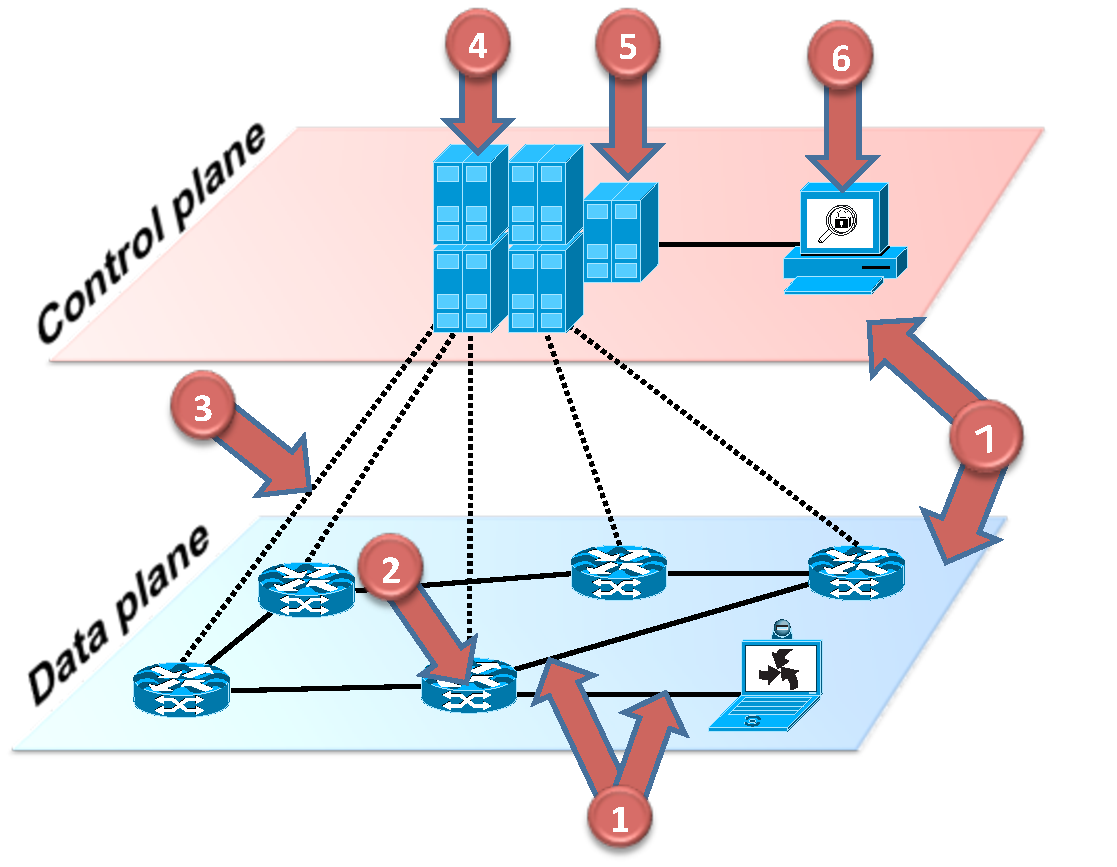
\includegraphics[width=0.85\columnwidth]{figures/fig9_sdn_threat_vectors.pdf}
\caption{Main threat vectors of SDN architectures}
\label{fig:threatvectorsmap}
\end{figure}

As can be observed in Table~\ref{tab:newandoldproblems}, threat vectors 3 to 5 are specific to SDN as they 
stem from the separation of the control and data planes and the consequent introduction of a new entity in 
these networks --- the logically centralized controller. The other vectors were already present 
in traditional networks. However, the impact of these threats could be larger than today --- or at least it 
may be expressed differently --- and as a consequence it may need to be dealt with differently.


{\renewcommand{\arraystretch}{1.4}
\begin{table}[!ht]
\caption{SDN specific vs. non-specific threats}
\label{tab:newandoldproblems}
\begin{center}
\footnotesize
%\rowcolors{1}{lightgray}{white}
\begin{tabularx}{\linewidth}{p{1.2cm}p{1.2cm}X}
\hline
\textbf{Threat vectors}  & \textbf{Specific to SDN?}  & \textbf{Consequences in software-defined networks} \\\hline
Vector 1      & no      & Open door for DDoS attacks.\\\hline
Vector 2      & no      & Potential attack inflation.\\\hline
Vector 3      & yes     & Exploiting logically centralized controllers.\\\hline
Vector 4      & yes     & Compromised controller may compromise the entire network.\\\hline
Vector 5      & yes     & Development and deployment of malicious applications on controllers. \\\hline
Vector 6      & no      & Potential attack inflation.\\\hline
Vector 7      & no      & Negative impact on fast recovery and fault diagnosis.\\
\hline
\end{tabularx}
\end{center}
\end{table}
}

OpenFlow networks are subject to a variety of security and dependability problems such as spoofing~\cite{kloti2013}, tampering~\cite{kloti2013}, 
repudiation~\cite{kloti2013}, information disclosure~\cite{kloti2013}, denial of service~\cite{kloti2013,shin2013,benton2013}, and elevation of privileges~\cite{kloti2013}.
The lack of isolation, protection, access control and stronger security recommendations~\cite{wasserman2013,shin2013,porras2012,benton2013} are some of the reasons for these vulnerabilities.
We will explore these next.

%In the remaining of this section we introduce the main threat vectors of SDN and practical security issues of current OpenFlow-enabled networks. Additionally, we discuss some countermeasures that should be consider to address different security and dependability problems of SDN/OpenFlow.

\vspace{2mm}
\noindent \textit{OpenFlow security assessment}

By applying the STRIDE methodology~\cite{hernan2006}, it is possible to identify different attacks to OpenFlow-enabled networks.
Table~\ref{tab:securitythreatsopenflow} summarizes these attacks (based on ~\cite{kloti2013}). 
For instance, information disclosure can be achieved through side channel attacks targeting the flow rule setup process. 
When reactive flow setup is in place, obtaining information about network operation is relatively easy.
An attacker that measures the delay experienced by the first packet of a flow and the subsequent can easily infer that the target network is a reactive SDN, and proceed with a specialized attack. 
This attack -- known as fingerprinting~\cite{shin2013} -- may be the first step to launch a DoS attack intended to exhaust the resources of the network, for example. 
If the SDN is proactive, guessing its forwarding rule policies is harder, but still feasible~\cite{kloti2013}. 
Interestingly, all reported threats and attacks affect all versions (1.0 to 1.3.1) of the OpenFlow specification. 
It is also worth emphasizing that some attacks, such as spoofing, are not specific to SDN. 
However, these attacks can have a larger impact in SDNs. 
For instance, by spoofing the address of the network controller, the attacker (using a fake controller) could  take over the control of the entire network. 
A smart attack could persist for only a few seconds, i.e., just the time needed to install special rules on all forwarding devices for its malicious purposes (e.g., traffic cloning). 
Such attack could be very hard to detect.

{\renewcommand{\arraystretch}{1.4}
\begin{table*}[!htp]
\caption{Attacks to OpenFlow networks.}
\label{tab:securitythreatsopenflow}
\begin{center}
\footnotesize
%\rowcolors{1}{lightgray}{white}
\begin{tabularx}{.85\textwidth}{ccX}
\hline
\textbf{Attack}  & \textbf{Security Property} & \textbf{Examples} \\\hline
\textbf{S}poofing & Authentication & MAC and IP address spoofing, forged ARP and IPv6 router advertisement\\\hline
\textbf{T}ampering & Integrity & Counter falsification, rule installation, modification affecting data plane.\\\hline
\textbf{R}epudiation & Non-repudiation & Rule installation, modification for source address forgery.\\\hline
\textbf{I}nformation disclosure & Confidentiality & Side channel attacks to figure out flow rule setup. \\\hline
\textbf{D}enial of service & Availability &  Flow requests overload of the controller. \\\hline
\textbf{E}levation of privilege & Authorization & Controller take-over exploiting implementation flaws. \\\hline
\end{tabularx}
\end{center}
\end{table*}
}

Taking counters falsification as another example, an attacker can try to guess installed flow 
rules and, subsequently, forge packets to artificially increase the counter.
Such attack would be specially critical for billing and load balancing systems, for instance.
A customer could be charged for more traffic than she in fact used, while a load balancing algorithm may take non-optimal decisions due to forged counters. 

Other conceptual and technical security concerns in OpenFlow networks include the lack of strong 
security recommendations for developers, the lack of TLS and access control support on most switch and controller 
implementations~\cite{wasserman2013}, the belief that TCP is enough because links are ``physically secure''~\cite{benton2013,wasserman2013}, the fact that many switches have listener 
mode activated by default (allowing the establishment of malicious TCP connections, for instance)~\cite{benton2013} or that flow table verification capabilities are harder to implement when TLS is not 
in use~\cite{wasserman2013,son2013}.
In addition, it is worth mentioning the high denial of service risk posed to centralized controllers~\cite{shin2013,son2013}, the vulnerabilities in the controllers themselves~\cite{son2013,kreutz2013}, and the risk of resource 
depletion attacks~\cite{shin2013,benton2013}.
For instance, it has been shown that an attacker can easily compromise control plane communications through 
DoS attacks and launch a resource depletion attack on control platforms by exploiting a single  application such as a learning switch~\cite{benton2013,shin2013}.

\vspace{2mm}
\noindent \textit{Countermeasures for OpenFlow based SDNs}

Several countermeasures can be put in place to mitigate the security threats in SDNs.
Table~\ref{tab:countermeasuresthreats} summarizes a number of countermeasures that can be applied to different 
elements of an SDN/OpenFlow-enabled network. Some of these measures, namely rate limiting, event filtering, 
packet dropping, shorter timeouts, and flow aggregation, are already recommended in more recent 
versions of the OpenFlow specification (version 1.3.1 and later). 
However, most of them are not yet supported or implemented in SDN deployments.

{\renewcommand{\arraystretch}{1.4}
\begin{table}[!htp]
\caption{Countermeasures for security threats in OpenFlow networks.}
\label{tab:countermeasuresthreats}
\begin{center}
\footnotesize
%\rowcolors{1}{lightgray}{white}
\begin{tabularx}{\columnwidth}{lX}
\hline
\multicolumn{1}{c}{\textbf{Measure}} & \multicolumn{1}{c}{\textbf{Short description}} \\\hline
Access control       & Provide strong authentication and authorization mechanisms on devices.  \\\hline
Attack detection     & Implement techniques for detecting different types of attacks. \\\hline
Event filtering         & Allow (or block) certain types of events to be handled by special devices. \\\hline
Firewall and IPS     & Tools for filtering traffic, which can help to prevent different types of attacks. \\\hline
Flow aggregation   & Coarse-grained rules to match multiple flows to prevent information disclosure and DoS attacks. \\\hline
Forensics support  & Allow reliable storage of traces of network activities to find the root causes of different problems.  \\\hline
Intrusion tolerance &  Enable control platforms to maintain correct operation despite intrusions. \\\hline
Packet dropping     & Allow devices to drop packets based on security policy rules or current system load. \\\hline
Rate limiting           & Support rate limit control to avoid DoS attacks on the control plane. \\\hline
Shorter timeouts  & Useful to reduce the impact of an attack that diverts traffic.  \\\hline
\end{tabularx}
\end{center}
\end{table}
}

Traditional techniques such as 
access control, attack detection mechanisms, event filtering (e.g.,  controller decides which asynchronous messages he is not going to accept), firewalls, and intrusion detection systems, can be used to mitigated the impact of or avoid attacks.
They can be implemented in different devices, such as controllers, forwarding devices, middleboxes, and so forth.
Middleboxes can be a good option for enforcing security policies in an enterprise because they are (in general) more robust and special purpose (high performance) devices.
Such a strategy also reduces the potential overhead cause by implementing these countermeasures directly on controllers or forwarding devices.
However, middleboxes can add extra complexity to the network management, i.e., increase the OPEX at the cost of a better performance.

Rate limiting, packet dropping, shorter timeouts and flow aggregations are techniques that can be applied on controlled and forwarding devices to mitigate different types of attacks, such as denial-of-service and information disclosure.
For instance, reduced timeouts can be used to mitigate the effect of an attack exploring the reactive operation mode of the network to make the controller install rules that divert traffic to a malicious machine. 
With reduced timeouts, the attacker would be forced to constantly generate a number of forged packets to avoid timeout expiration, making the attack more likely to be detected.
Rate limiting and packet dropping can be applied to avoid DoS attacks on the control plane or stop on-going attacks directly on the data plane by installing specific rules on the devices where the attacks is being originated.

Forensics and remediation encompass mechanisms such as secure logging, event correlation and consistent reporting. 
If anything wrong happens with the network, operators should be able to safely figure out the root cause of the problem and put the network to work on a secure operation mode as fast as possible.
Additionally, techniques to tolerate faults and intrusions, such as state machine replication~\cite{bolosky2011}, proactive-reactive recovery~\cite{sousa2010}, and diversity~\cite{garcia2013}, can be added to control platforms for increasing the robustness and security properties by automatically masking and removing faults.
Put differently, SDN controllers should be able to resist against different types of events (e.g., power outages, network disruption, communication failures, network partitioning) and attacks (e.g., DDoS, resource exhaustion)~\cite{kreutz2013,botelho2013}. 
One of the most traditional ways of achieving high availability is through replication. 
Yet, proactive-reactive recover and diversity are two examples of crucial techniques that add value to the system for resisting against different kinds of attacks and failures (e.g., those exploring common vulnerabilities or caused by software aging problems).

Other countermeasures to address different threats and issues of SDN include enhancing the security and 
dependability of controllers, protection and isolation of applications~\cite{sorensen2012,kreutz2013,porras2012}, trust management between controllers 
and forwarding devices~\cite{kreutz2013}, integrity checks of controllers and applications~\cite{kreutz2013}, forensics and remediation~\cite{sorensen2012,kreutz2013}, 
verification frameworks~\cite{chua2013,porras2012,korniak2011}, and resilient control planes~\cite{fonseca2012,korniak2011,kreutz2013,sorensen2012}.
Protection and isolation mechanisms should be part of any controller. Applications should be isolated from each other and from the controller. 
Different techniques such as security domains (e.g., kernel, security, and user level) and data access protection mechanisms should be put in place in order to avoid security threats from management applications. 

Implementing trust between controllers and forwarding is another requirement for insuring that malicious elements 
cannot harm the network without being detected. 
An attacker can try to spoof the IP address of the controller and make switches connect to its own controller. 
This is currently the case since most controllers and switches only establish insecure TCP connections. 
Complementarly, integrity checks on controller and application software can help to ensure that safe code is being bootstrapped, which eliminates harmful software from being started once the system restarts. 
Besides integrity checks, other things such as highly specialized malware detection systems should be developed for SDN. 
Third-party management applications should always be scanned for bad code and vulnerabilities because a malicious application represents a significant security threat to the network. 

It is worth mentioning that there are also other approaches for mitigating security threats in SDN, such as declarative languages to eliminate network 
protocol vulnerabilities~\cite{casey2013}. 
This kind of descriptive languages can specify semantic constraints, structural constraints and safe access properties of OpenFlow messages. 
Then, a compiler can use these inputs to find programmers' implementation mistakes on message operations. 
In other words, such languages can help find and eliminate implementation vulnerabilities of southbound specifications.

\subsection{Migration to SDN}
\label{sec:hybrid}

A prime SDN adoption challenge relates to organizational barriers that may arise due to the first (and second) order 
effects of SDN automation capabilities and ``layer/domain blurring''. 
Some level of human resistance is to be expected and may affect the decision and deployment processes of SDN, especially by those that may regard the 
control refactorization of SDN as a risk to the current chain of control and command, or even to their job security. 
This complex social challenge is similar (and potentially larger) to known issues between the transport and IP 
network divisions of service providers, or the system administrator, storage, networking, and security teams 
of enterprise organizations. Such a challenge is observable on today's virtualized data centers, through the shift 
in role and decision power between the networking and server people. Similarly, the development and operations (DevOps) movement has caused a shift in the locus of influence, not only 
on the network architecture but also on purchasing, and this is an effect that SDN may exacerbate. These changes in role and power causes a second order effect on the sales division of vendors that are required to adapt accordingly. 


Pioneering SDN operational deployments have been mainly greenfield scenarios and/or tightly controlled single 
administrative domains. Initial roll-out strategies are mainly based on virtual switch overlay models or 
OpenFlow-only network-wide controls. However, a broader adoption of SDN beyond data center silos -- and 
between themselves -- requires considering the interaction and integration with legacy control planes providing 
traditional switching; routing; and operation, administration, and management (OAM) functions. Certainly, 
rip-and-replace is not a viable strategy for the broad adoption of new networking technologies.

Hybrid networking in SDN should allow deploying OpenFlow for a subset of all flows only, enable OpenFlow on 
a subset of devices and/or ports only, and provide options to 
interact with existing OAM protocols, legacy devices, and neighboring domains. As in any technology transition 
period where fork-lift upgrades may not be a choice for many, migration paths are critical for 
adoption.

Hybrid networking in SDN spans several levels. The Migration Working Group of the ONF is tackling the scenario where hybrid switch architectures and hybrid (OpenFlow and non-OpenFlow) devices 
co-exist. Hybrid switches can be configured to behave as a legacy switch or as an OpenFlow switch and, in some 
cases, as both simultaneously. This can be achieved, for example, by partitioning the set of ports of a switch, 
where one subset is devoted to OpenFlow-controlled networks, and the other subset to legacy networks. For these 
subsets to be active at the same time, each one having its own data plane, multi-table support at the forwarding 
engine (e.g., via TCAM partitioning) is required. Besides port-based partitioning, it is also possible to rely 
on VLAN-based (prior to entering the OpenFlow pipeline) or flow-based partitioning using OpenFlow matching and 
the \texttt{LOCAL} and/or \texttt{NORMAL} actions to redirect packets to the legacy pipeline or the switch's 
local networking stack and its management stack. Flow-based partitioning is the most flexible option, as it 
allows each packet entering a switch to be classified by an OpenFlow flow description and treated by the 
appropriate data plane (OpenFlow or legacy).

The promises by SDN to deliver easier design, operation and management of computer networks are endangered
by challenges regarding incremental deployability, robustness, and scalability. Full SDN deployments are 
difficult and straightforward only in some green field deployments such as data center networks or by 
means of an overlay model approach. Hybrid SDN approaches represent however a very likely deployment model 
that can be pursued by different means, including~\cite{vissicchio2014}:

\begin{itemize}
\item Topology-based hybrid SDN: Based on a topological separation of the nodes controlled by traditional and SDN 
paradigms. The network is partitioned in different zones and each node belongs to only one zone. 
\item Service-based hybrid SDN: Conventional networks and SDN provide different services, where overlapping nodes, 
controlling a different portion of the FIB (or generalized flow table) of each node. Examples include network-wide 
services like forwarding  that can be based on legacy distributed control, while SDN provides edge-to-edge services 
such as enforcement of traffic engineering and access policies, or services requiring full traffic visibility 
(e.g., monitoring).
\item Class-based hybrid SDN: Based on the partition of traffic in classes, some controlled by SDN and the remaining 
by legacy protocols. While each paradigm controls a disjoint set of node forwarding entries,  each paradigm is 
responsible for all network services for the assigned traffic classes. 
\item Integrated hybrid SDN: A model where SDN is responsible for all the network services, and
uses traditional protocols (e.g., BGP) as an interface to node FIBs. For example, it can control forwarding
paths by injecting carefully selected routes into a routing system or adjusting protocol settings (e.g., IGP weights). 
Past efforts on RCPs~\cite{caesar2005} and the ongoing efforts within ODL~\cite{opendaylight2013} can be considered 
examples of this hybrid model.
\end{itemize}

In general, benefits of hybrid approaches include enabling flexibility (e.g., easy match on packet fields for 
middleboxing) and SDN-specific features (e.g., declarative management interface) while partially keeping the inherited 
characteristics of conventional networking such as robustness, scalability, technology maturity, and low deployment 
costs. On the negative side, the drawbacks of hybridization include the need for ensuring profitable interactions 
between the networking paradigms (SDN and traditional) while dealing with the heterogeneity that largely depends on 
the model.

Initial trade-off analyses suggest that the combination of centralized and distributed paradigms may provide 
mutual benefits. However, future work is required to devise techniques and interaction mechanisms that maximize 
such benefits while limiting the added complexity of the paradigm coexistence.

Some efforts have been already devoted to the challenges of migration and hybrid SDNs. RouteFlow~\cite{rothenberg2012-1} implements an IP level control plane on top of an OpenFlow 
network, allowing the underlying devices to act as IP routers under different possible arrangements. LegacyFlow 
\cite{rothenberg2014} extends the OpenFlow-based controlled network to embrace non-OpenFlow nodes. The common 
grounds of these pieces of work are (1) considering hybrid as the coexistence of traditional environments of 
closed vendor's routers and switches with new OpenFlow-enabled devices; (2) targeting the interconnection of 
both control and data planes of legacy and new network elements; and (3) taking a controller-centric approach, 
drawing the hybrid line outside of any device itself, but into the controller application space.

Panopticon~\cite{levin2014} defines an architecture and methodology to consistently implement 
SDN inside enterprise legacy networks through network orchestration under strict budget constraints. The proposed 
architecture includes policy configurations, troubleshooting and maintenance tasks establishing transitional networks 
(SDN and legacy) in structures called Solitary Confinement Trees (SCTs), where VLAN IDs are efficiently used by 
orchestration algorithms to build paths in order to steer traffic through SDN switches. Defying the partial SDN 
implementation concept, they confirm that this could be a long-term operational strategy solution for enterprise 
networks.

HybNET~\cite{lu2013} presents a network management framework for
hybrid OpenFlow-legacy networks. It provides a common centralized
configuration interface to build virtual networks using VLANs. An
abstraction of the physical network topology is taken into account by
a centralized controller that applies a path finder mechanism, in
order to calculate network paths and program the OpenFlow switches via
REST interfaces~\cite{richardson2008restful} and legacy devices using NETCONF~\cite{enns2011-1}.

\subsection{SDN for telecom and cloud providers}

A number of carrier-grade infrastructure providers (e.g., NTT, AT\&T, Verizon, Deutsch Telekom) have already joined the SDN community and its activities with the ultimate goal of solving their long standing networking problems.
One of the forefront runners (and early SDN adopter) was NTT, already taking advantage o this new paradigm to provide new on-demand network provisioning models.
In 2013, NTT launched an SDN-based, on-demand elastic provisioning platform of network resources (e.g., bandwidth) for HD video broadcasters~\cite{bernier2013}. 
Similarly, as a global cloud provider with data centers spread across the globe~\cite{nttdata2014}, the same company launched a similar service for its cloud customers, who are now capable of taking advantage of dynamic networking 
provisioning intra- and inter-data centers~\cite{wagner2014}.
AT\&T is another telecom company that is investing heavily in new services, such as user-defined network clouds, that 
take advantage of recent developments in NFV and SDN~\cite{atandtinc.2014}.
These are some of the early examples of the opportunities SDNs seem to bring to telecom and cloud providers. 

Carrier networks are using the SDN paradigm as the technology means for solving a number of long standing problems. 
%in an easier way, such as inter-data center over-provisioned router links, static allocation 
%of circuit-switched links, isolation of operation by network layers, separated management of L3/L2 and L1 
%infrastructure (which causes lots of extra costs by requiring multiple sets of  people  to  operate them - engineering,    planning, provisioning), fine-grained QoS, and network virtualization. 
Some of these efforts include 
new architectures for a smooth migration from the current mobile core infrastructure to SDN~\cite{pentikousis2013}, and techno-economic models for virtualization of these networks~\cite{naudts2012,onfsolutionbrief2013};  
carrier-grade OpenFlow virtualization schemes~\cite{skoldstrom2013,koponen}, including virtualized broadband access infrastructures~\cite{gharakheili2013}, techniques that are allowing the offer of network-as-a-service~\cite{pacnet2013}; 
flexible control of network resources~\cite{corporation2012}, including offering MPLS services using an SDN approach~\cite{das2011};
and the investigation of novel network architectures, from proposals to separate the network edge from the core~\cite{casado2012,6786608}, with the latter forming the fabric that transports packets as defined by an intelligent edge, to software-defined Internet exchange points~\cite{feamster2013,stringer2013}.


SDN technology also brings new possibilities for cloud providers.
By taking advantage of the logically centralized control of network resources~\cite{hong2013,jain2013-1} it is possible to simplify and optimize network management of data centers and achieve:
(i) efficient intra-datacenter networking, including fast recovery mechanisms for the  data and control planes~\cite{sharma2013-1,staessens2011,sharma2013}, simplified fault-tolerant routing~\cite{mysore2009}, performance isolation~\cite{greenberg2009}, and easy and efficient resource migration (e.g., of VMs and virtual networks)~\cite{sharma2013-1};
(ii) improved inter-datacenter communication, including the ability to fully utilize the expensive high-bandwidth links without impairing quality of service~\cite{jain2013-1,sadasivarao2013};
(iii) higher levels of reliability (with novel fault management mechanisms, etc.)~\cite{mysore2009,sharma2013-1,staessens2011}; and 
(iv) cost reduction by replacing complex, expensive hardware by simple and cheaper forwarding devices~\cite{tanner2013,jain2013-1}.

Table~\ref{tab:carriergradeneeds} summarizes some of the carrier-grade network and cloud infrastructure providers' requirements.
In this table we show the current challenges and what is to be expected with SDN.
As we saw before, some of the expectations are already becoming a reality, but many are still open issues.
What seems to be clear is that SDN represents an opportunity for telecom and cloud providers, in providing flexibility, cost-effectiveness, and easier management of their networks.


{\renewcommand{\arraystretch}{1.4}
\begin{table*}[t!]
\caption{Carrier-grade and cloud provider expectations \& challenges}
\label{tab:carriergradeneeds}
\newcommand{\firstcolumnwidth}{2.5cm} 
\begin{center}
\footnotesize
\begin{tabularx}{0.99\textwidth}{p{\firstcolumnwidth}p{6cm}X}
\hline
\textbf{What} & \textbf{Currently} & \textbf{Expected with SDN} \\\hline
\multirow{8}{*}{\begin{minipage}{\firstcolumnwidth}Resource Provisioning\end{minipage}} 
                     & Complex load balancing configuration. & Automatic load balancing reconfiguration.~\cite{elby2012,jain2013-1} \\\cline{2-3}
		    & Low virtualization capabilities across hardware platforms & NFV for virtualizing network functionality across hardware appliances.~\cite{tanner2013,atandtinc.2014} \\\cline{2-3}
		    & Hard and costly to provide new services. & Create and deploy new network service quickly.~\cite{tanner2013,atandtinc.2014}\\\cline{2-3}
                     & No bandwidth on demand. & Automatic bandwidth on demand.~\cite{onfsolutionbrief2013} \\\cline{2-3}
                     & Per network element scaling. & Better incremental scaling.~\cite{elby2012,staessens2011} \\\cline{2-3}
		    & Resources statically pre-provisioned. & Dynamic resource provisioning in response to load.~\cite{elby2012,jain2013-1,tanner2013,naudts2012,hong2013} \\
\hline
\multirow{4}{*}{\begin{minipage}{\firstcolumnwidth}Traffic Steering\end{minipage}} 
                     & All traffic is filtered. & Only targeted traffic is filtered.~\cite{elby2012} \\\cline{2-3}
                     & Fixed only. & Fixed and mobile.~\cite{elby2012} \\\cline{2-3}
                     & Per network element scaling. & Better incremental scaling. ~\cite{naudts2012,staessens2011}\\\cline{2-3}
                     & Statically configured on a per-device basis. & Dynamically configurable.~\cite{jain2013-1,onfsolutionbrief2013,anwer2013} \\
\hline
\multirow{4}{*}{\begin{minipage}{\firstcolumnwidth}Ad Hoc Topologies\end{minipage}}   
                     & All traffic from all probes collected. & Only targeted traffic from targeted probes is collected. \\\cline{2-3}
                     & Massive bandwidth required. & Efficient use of bandwidth.~\cite{jain2013-1,onfsolutionbrief2013} \\\cline{2-3}
                     & Per network element scaling. & Better incremental scaling.~\cite{elby2012,onfsolutionbrief2013} \\\cline{2-3}
                     & Statically configured. & Dynamically configured.~\cite{elby2012,gerlach2013,bernier2013} \\
\hline
\multirow{7}{*}{\begin{minipage}{\firstcolumnwidth}Managed Router\\ Services\end{minipage}}   
                     & Complex configuration, management and upgrade. & Simplified management and upgrade.~\cite{jain2013-1,elby2012,tanner2013,onfsolutionbrief2013,staessens2011} \\\cline{2-3}
                     & Different kinds of routers, such as CO. & No need for CO routers, reducing aggregation costs.~\cite{elby2012,tanner2013,naudts2012} \\\cline{2-3}
                     & Manual provisioning. & Automated provisioning.~\cite{elby2012,onfsolutionbrief2013,anwer2013} \\\cline{2-3}
                     & On-premises router deployment. & Virtual routers (either on-site or not).~\cite{onfsolutionbrief2013,elby2012,naudts2012} \\\cline{2-3}
                     & Operational burden to support different equipments. & Reduced technology obsolescence.~\cite{naudts2012} \\\cline{2-3}
                     & Router change-out as technology or needs change. & Pay-as-you grow CAPEX model.~\cite{naudts2012} \\\cline{2-3}
                     & Systems complex and hard to integrate. & Facilitates simplified system integrations.~\cite{elby2012,tanner2013,gerlach2013}\\\hline
\multirow{2}{*}{\begin{minipage}{\firstcolumnwidth}Revenue Models\end{minipage}}   
                     & Fixed long term contracts. & More flexible and on-demand contracts.~\cite{onfsolutionbrief2013,corporation2012}\\\cline{2-3}
                     & Traffic consumption. & QoS metrics per-application.~\cite{onfsolutionbrief2013,staessens2011,staessens2011,velasco2013} \\
\hline
\multirow{4}{*}{\begin{minipage}{\firstcolumnwidth}Middleboxes \\Deployment \& \\Management\end{minipage}}   
                     & Composition of services is hard to implement. & Easily expand functionality to meet the infrastructure needs.~\cite{tanner2013}\\\cline{2-3}
                     & Determine where to place middleboxes a priori (e.g., large path inflation problems). & Dynamic placement using shortest or least congested path. ~\cite{qazi2013-1,velasco2013,gerlach2013} \\\cline{2-3}
                     & Excessive over-provisioning to anticipate demands. & Scale up to meet demands, and scale down to conserve resources (elastic middleboxes).~\cite{elby2012,naudts2012} \\
\hline
\multirow{3}{*}{\begin{minipage}{\firstcolumnwidth}Other Issues\end{minipage}}   
                     & Energy saving strategies are hard to implement. & Flexible and easy to deploy energy saving strategies.~\cite{staessens2011}\\\cline{2-3}
                     & Complex and static control and data plane restoration techniques. & Automated and flexible restoration techniques for both control and data plane.~\cite{staessens2011}\\\cline{2-3}
\hline
\end{tabularx}
\end{center}
\end{table*}
}

%For instance, telecom providers such as Verizon 
%~\cite{elby2012} foresee several advantages and improvements for carrier-grade network infrastructures.
%Examples include implementation of network functions on COTS hardware, virtualization of network functions,
%application and service aware routing, orchestration of network and cloud resources,
%added efficiency on the network, and on-demand virtual network resource provisioning. 
%Use-cases range from dynamic resource provisioning, automatic load balancing reconfiguration, traffic steering (e.g., targeted traffic 
%filtering, incremental network scaling per device), ad-hoc network topologies with QoS assurance, to integration 
%of new functions in the network.

\subsection{SDN: the missing piece towards Software-Defined Environments}

The convergence of different technologies is enabling the emergence of fully programmable IT infrastructures.
It is already possible to dynamically and automatically configure or reconfigure the entire IT stack, from the network infrastructure up to the applications, to better respond to workload changes.
Recent advances makes on-demand provisioning of resources possible, at nearly all infrastructural layers.
The fully automated provisioning and orchestration of IT infrastructures as been recently named Software-Defined Environments (SDEs)~\cite{racherla2014,li2014}, by IBM.
This is a novel approach that is expected to have significant potential in simplifying IT management, optimizing the use of the infrastructure, reduce costs, 
and reduce the time to market of new ideas and products.
In an SDE, workloads can be easily and automatically assigned to the appropriate IT resources based on application characteristics, security and service level policies, and the best-available resources to deliver continuous, dynamic optimization and reconfiguration to address infrastructure issues in a rapid and responsive manner.
Table~\ref{tab:TraditionalAndSDE} summarizes the traditional approaches and some of the key features being enabled 
by SDEs~\cite{alba2014,arnold2014}.

{\renewcommand{\arraystretch}{1.4}
\begin{table*}[t!]
\caption{SDE pushing IT to the next frontier}
\label{tab:TraditionalAndSDE}
\newcommand{\firstcolumnwidth}{3.2cm} 
\begin{center}
\footnotesize
\begin{tabularx}{0.99\textwidth}{XX}
\hline
\textbf{Traditionally} & \textbf{Expected with SDEs} \\\hline
IT operations manually map the resources for apps for software deployment.  & Software maps resources to the workload and deploys the workload. \\\hline
Networks are mostly statically configured and hard to change.  & Networks are virtualized and dynamically configured on-demand. \\\hline
Optimization and reconfiguration to reactively address issues are manual.  & Analytics-based optimization and reconfiguration of infrastructure issues. \\\hline
Workloads are typically manually assigned to resources.  & Workloads are dynamically assigned. \\\hline
%\\\hline
\end{tabularx}
\end{center}
\end{table*}
}

In an SDE the workloads are managed independently of the systems and underlying infrastructure, i.e., are not tied to a specific technology or vendor~\cite{li2014,racherla2014}.
Another characteristic of this new approach is to offer a programmatic access to the environment as a whole, selecting the best available resources based on the current status of the infrastructure, and enforcing the policies defined.
In this sense, it shares much of the philosophy of SDN.
Interestingly, one of the missing key pieces of an SDE was, until now, Software-Defined Networking.

The four essential building blocks of an SDE~\cite{li2014,racherla2014,arnold2014} are:

\begin{itemize}
\item Software-Defined Networks (SDN)~\cite{dixon2014,ibmsystemsandtechnologygroup2014},
\item Software-Defined Storage (SDS)~\cite{alba2014},
\item Software-Defined Compute (SDC)~\cite{racherla2014}, and 
\item Software-Defined Management (SDM)~\cite{ibmsystems2014}.
\end{itemize}

In the last decade the advances in virtualization of compute and storage, together with the availability of sophisticated cloud orchestration tools have enabled SDS, SDC and SDM.
These architectural components have been widely used by cloud providers and for building IT infrastructures in different enterprise environments.
However, the lack of programmable network control has so far hindered the realization of a complete Software-Defined Environment.
SDN is seen as the technology that may fill this gap, as attested by the emergence of cloud-scale network virtualization platforms based on this new paradigm~\cite{koponen}.

%SDEs are becoming, at a relatively fast pace, key orchestration systems to drive IT management to the next 
%level, changing the long standing essential static or manually setup of the infrastructure and systems to 
%accommodate diverse and dynamic workloads. 
%Traditionally, IT infrastructures have been quite complex and hard to manage and evolve, and in particular 
%the network. For instance, workloads are typically manually assigned to resources, networks are mostly statically 
%configured and hard to change, IT operations manually map the resources for applications for software deployment, optimization and reconfiguration to reactively address issues are also manual.


%Traditionally:
%workloads are typically manually assigned to resources;
%networks are mostly statically configured and hard to change;
%IT operations manually map the resources for applications for software deployment;
%optimization and reconfiguration to reactively address issues are also manual.
%
%with SDEs:
%workloads are dynamically assigned;
%networks are virtualized and dynamically configured in an on-demand fashion;
%Software maps resources to the workload and deploys the workload;
%Analytics-based optimization and reconfiguration address infrastructure issues.
%

% Figure: SDE-enabled IT infrastructure overview.
\begin{figure}[ht!]
\centering
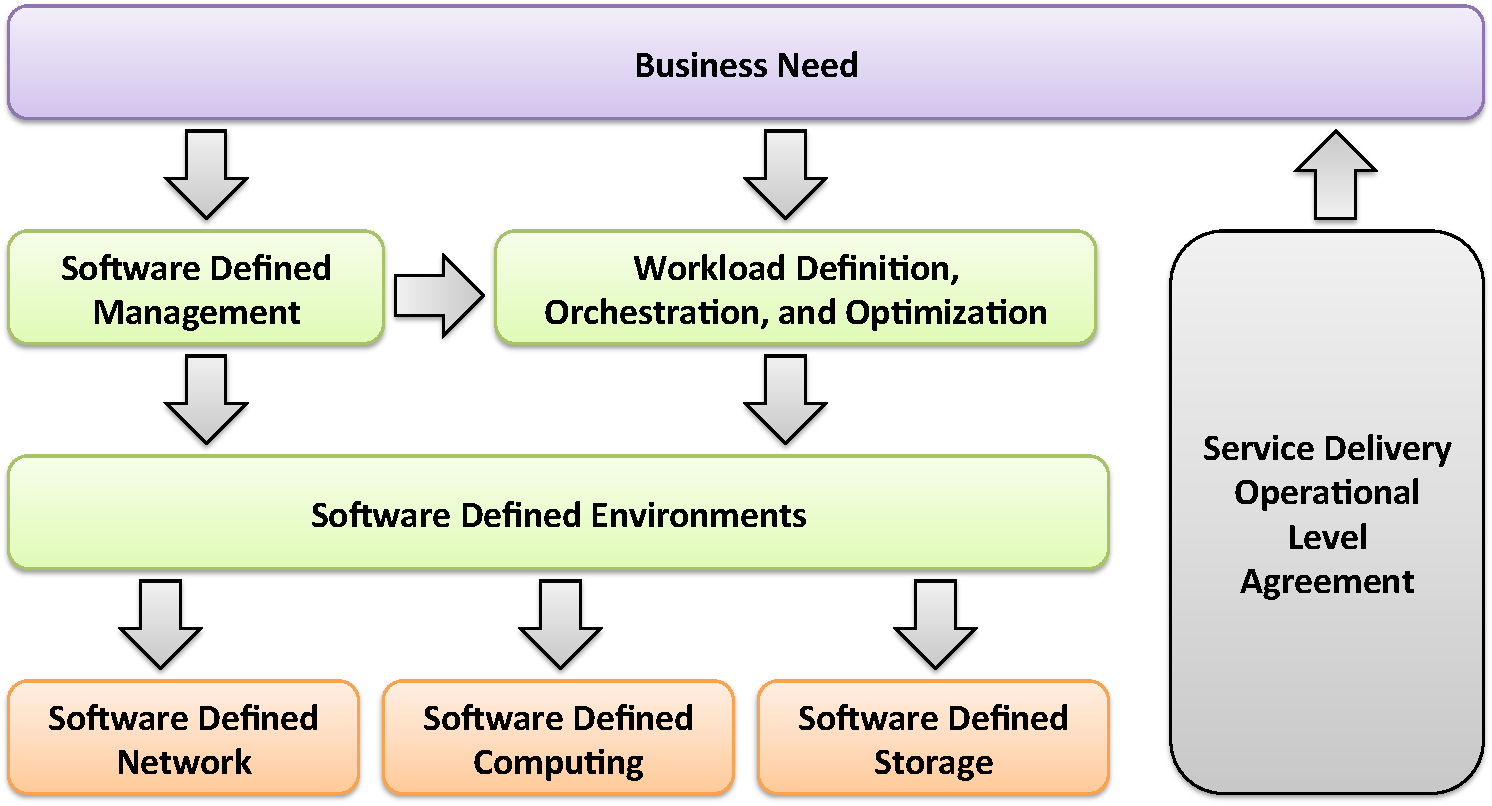
\includegraphics[width=0.95\columnwidth]{figures/fig10_sde_enabled_IT.pdf}
\caption{Overview of an IT infrastructure based on a SDE.}
\label{fig:SDEenabledIT}
\end{figure}


The IBM SmartCloud Orchestrator is one of the first examples of an SDE~\cite{li2014,racherla2014}.
It integrates compute, storage, management and networking in a structured way
Figure~\ref{fig:SDEenabledIT} gives a simplified overview of an SDE, by taking the approach developed by IBM as its basis.
The main idea of an SDE-based infrastructure is that the business needs that define the workloads trigger the reconfiguration of the global IT infrastructure (compute, storage, network). 
This is an important step towards a more customizable IT infrastructure that focuses on the business requirements rather than on the limitations of the infrastructure itself.


% FIXME: XXXXX

%It is worth to emphasize that SDN plays a major key role in enabling SDEs.
%Currently, vendors take advantage of the flexibility and programmability provided by controllers on the control plane to optimize network resources utilization to achieve high performance and competitive advantages. 
%The forwarding devices-based control plane paradigm gives network administrators a first opportunity to fix the bleeding need of increasing data flow efficiency across the network as a whole.

%Nowadays, with SDN, instead of thinking the network as a monolithic, complex and hard to evolve infrastructure, 
%one can now think about the network as a software platform. The evolution of the network is now limited mostly 
%by the software (e.g., applications), i.e., network functions and protocols are driven by fast evolving software 
%components, which provides a greater flexibility and a very fast pace of evolution when compared to traditional
%networks. Moreover, it is much easier to integrate the network control with higher-level software stacks, such 
%as hypervisors and cloud orchestration. Figure~\ref{fig:SDNandSDE} illustrates how SDN can fit in the new 
%software enabled IT infrastructures~\cite{racherla2014}.

% Figure: relationship of SDN and the SDE.
%\begin{figure}[ht!]
%\centering
%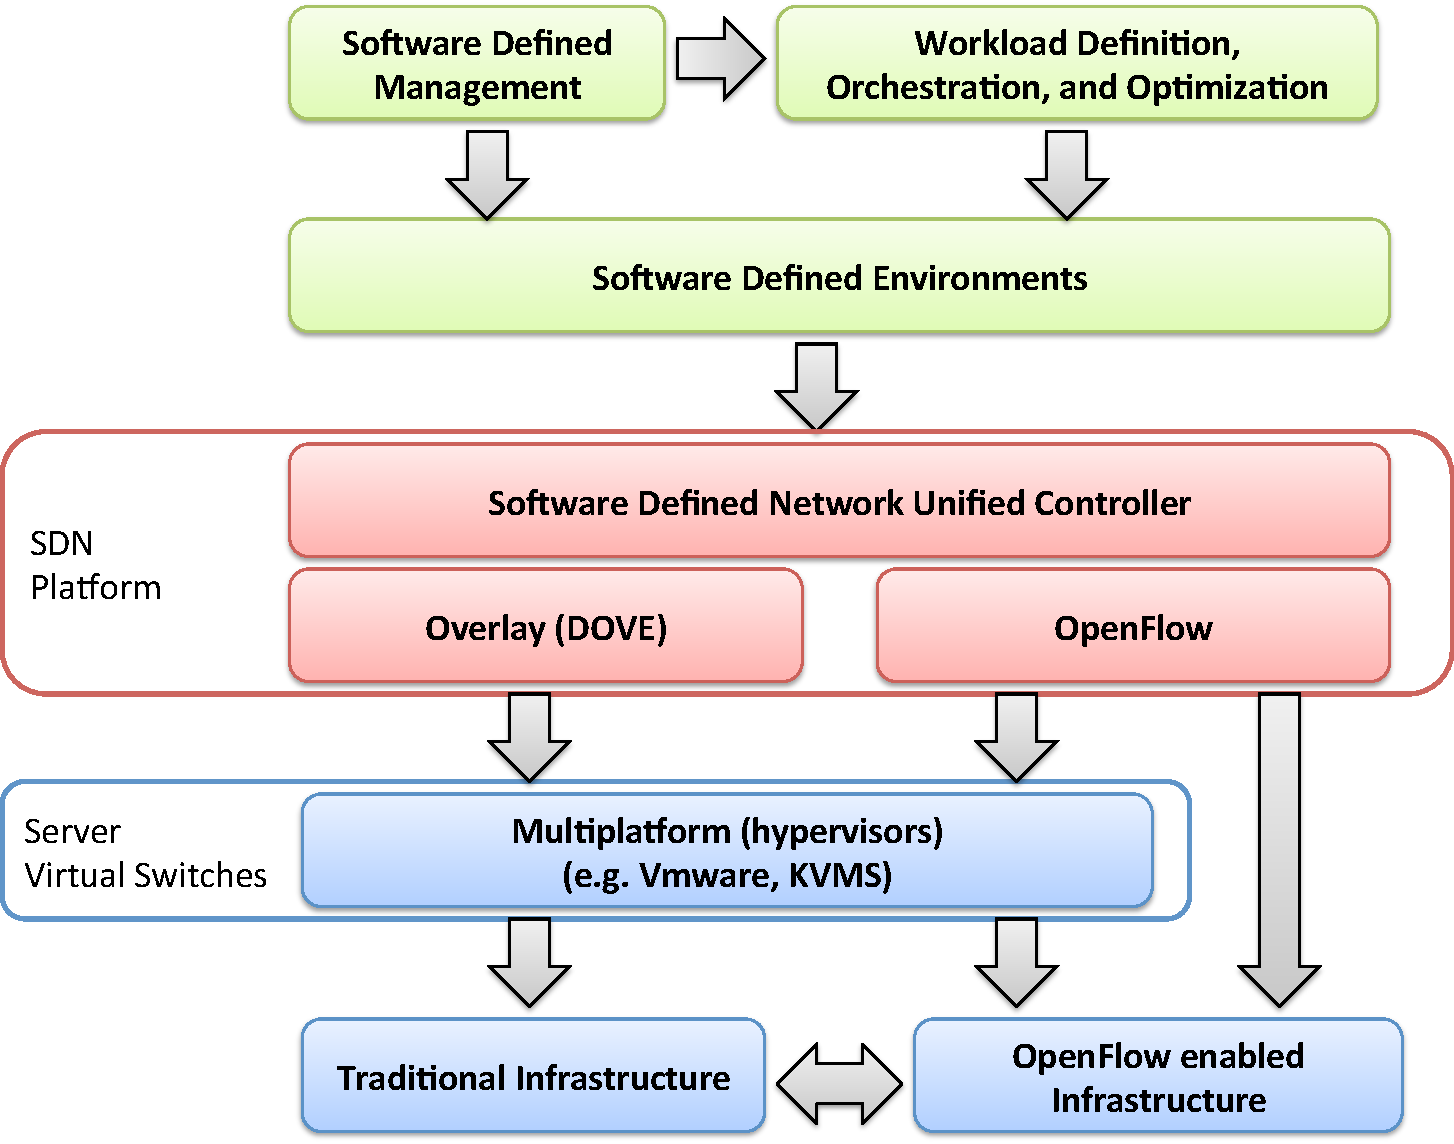
\includegraphics[width=0.95\columnwidth]{figures/fig11_sde_and_sdn.pdf}
%\caption{SDN completing the puzzle of an SDE.}
%\label{fig:SDNandSDE}
%\end{figure}

%The SDN Unified Controller represents IBM's approach for using SDN as one of the essential building blocks 
%for the next generation of SDEs. There are different concerns and driving forces of SDN into this new world 
%of SDEs. First, SDN is an obvious useful tool for helping to consolidate and virtualize server platforms and 
%network resources. Some of the main trade-offs in merging server and network virtualization is directly related 
%with the enforcement of security policies. On one hand, we have several driving forces toward highly 
%efficient systems. On the other hand, we need to guarantee security isolation and QoS guarantees for the 
%virtual networks of tenants. SDN helps tackle these issues by making it possible for security control 
%enforcement elements to be placed in the right place, i.e., where it makes more sense in terms of computing 
%needs and network flows. Second, cost reduction has always been one of the major forces that is driven by the 
%global economy, always putting some sort of stress on the enterprise IT budgets. Therefore, IT projects that 
%are not capable of demonstrating the added-value for the business have day-after-day less chance to succeed.
%SDN can be used as a key tool to demonstrate that business can now experience a decreasing time to market thanks 
%to (1) dynamic and fast resource provisioning mechanisms, (2) a reduced capital expenditure by shifting the costs 
%from intelligent and expensive hardware devices to software running on top of commodity server platforms, and 
%(3) reduced overall operational expenses through a global blueprint of what is running on the infrastructure 
%without the hassle of having to manage diverse systems commonly controlled by specific, proprietary and complex 
%protocols and tools. Put differently, SDN makes enterprise LANs shift from locked-in and complex solutions to 
%a model where the forwarding devices functionality is a common and simple enough industry accepted standard to 
%make multi-vendor networks an attractive solution for clients.

%It is also worth emphasizing that in this new virtualized and highly integrated world, it is important that 
%data center professionals have a broad knowledge. These professionals have now to know about a variety of 
%technologies and new concepts such as hypervisors, storage, computing virtualization, storage virtualization, 
%network virtualization, software-defined networks, security, elasticity of computing, storage and networking 
%resources, full environment migration, and so forth. Most importantly, IT sections of enterprise cannot be organized 
%anymore into independent silos. The interdependencies between the different infrastructure layers, technologies 
%and resources have reached their peak. For instance, SDEs are driving a major change in computing and networking 
%infrastructure, where applications at the top level start to define the computing, storage and networking 
%resources. Therefore, it is more than critical to have a global and collective view of what is available in 
%the infrastructure for business applications and systems. Naturally, it implies in new skills and 
%multidisciplinary approaches, which are not yet a common case in IT organizations. In fact, many times, there 
%is some resistance between different teams (e.g., security and network infrastructure, development and security, 
%development and network infrastructure, IT business requirements and IT infrastructure teams and/or providers) 
%to interact and be flexible enough to understand and try out smart solution to a variety of interesting, and 
%sometimes complicated, problems.

%It seems clear that the key pieces for SDE can finally be put together. More importantly, 
%the missing piece of this complex puzzle, SDN, is finally under a fast pace development and evolution. However, 
%there is still a long way and many interesting challenges in designing, implementing and deploying SDEs. IBM took 
%the first step in this direction by providing commercial products capable of delivering some of the exciting 
%features of these new dynamically programmable environments, focusing always on the business and application 
%requirements, rather than putting IT as a barrier to the business evolution.
%\input{text/6_domains.tex}
%\input{text/7_open_roads.tex}
%\input{text/7_killer_apps.tex}
%% Conclusion
\section{Conclusion}

Traditional networks are complex and hard to manage.  One
of the reasons is that the control and data planes are vertically
integrated and vendor specific. Another, concurring reason, is that
typical networking devices are also tightly tied to line products and
versions.  In other words, each line of product may have its own
particular configuration and management interfaces, implying long
cycles for producing product updates (e.g., new firmware) or upgrades
(e.g., new versions of the devices). All this has given rise to vendor
lock-in problems for network infrastructure owners, as well as posing
severe restrictions to change and innovation.

Software-Defined Networking (SDN) created an opportunity for solving
these long-standing problems.  Some of the key ideas of SDN are the
introduction of dynamic programmability in forwarding devices through
open southbound interfaces, the decoupling of the control and data
plane, and the global view of the network by logical centralization of
the ``network brain''.  While data plane elements became dumb, but
highly efficient and programmable packet forwarding devices, the
control plane elements are now represented by a single entity, the
controller or network operating system.  Applications implementing the
network logic run on top of the controller and are much easier to
develop and deploy when compared to traditional networks. Given the
global view, consistency of policies is straightforward to enforce.
SDN represents a major paradigm shift in the development and
evolution of networks, introducing a new pace of innovation in networking infrastructure.

In spite of recent and interesting attempts to survey this new chapter
in the history of networks~\cite{lara2014,jarraya2014,nunes2014}, the
literature was still lacking, to the best of our knowledge, a single
extensive and comprehensive overview of the building blocks, concepts,
and challenges of SDNs.
%
%% , such as network operating systems, network hypervisors,
%% programming languages, scalability and security challenges,
%% debugging and troubleshooting, challenges and open roads.
%
Trying to address this gap, the present paper used a layered approach
to methodically dissect the state of the art in terms of concepts,
ideas and components of software-defined networking, covering a broad
range of existing solutions, as well as future directions.

We started by comparing this new paradigm with traditional networks
and discussing how academy and industry helped shape software-defined
networking.  Following a bottom-up approach, we provided an in-depth
overview of what we consider the eight fundamental facets of the SDN
problem: 1) hardware infrastructure, 2) southbound interfaces, 3)
network virtualization (hypervisor layer between the forwarding
devices and the network operating systems), 4) network operating
systems (SDN controllers and control platforms), 5) northbound
interfaces (common programming abstractions offered to network
applications), 6) virtualization using slicing techniques provided by
special purpose libraries and/or programming languages and compilers,
7) network programming languages, and finally, 8) network
applications.

%%PJV:  please someone clarify content of (6) w.r.t. ``virtualization'' in (3) but is a more concise way

SDN has successfully managed to pave the way towards a next generation networking, spawning an innovative research and development
environment, promoting advances in several areas: switch and
controller platform design, evolution of scalability and performance
of devices and architectures, promotion of security and dependability.

We will continue to witness extensive activity around SDN in the near
future. Emerging topics requiring further research are, for example:
the migration path to SDN, extending SDN towards carrier transport networks, realization of the
network-as-a-service cloud computing paradigm, or software-defined
environments (SDE).
\coloredtext{As such, we would like to receive feedback from the networking/SDN community as this novel paradigm evolves, to make this a ``live document'' that gets updated and improved based on the community feedback.
We have set up a github page\footnote{\coloredtext{https://github.com/SDN-Survey/latex/wiki}} for this purpose, and we invite our readers to join us in this communal effort.}

\begin{comment}

Traditional networks have always been complex and hard to manage.  One
of the reasons is that the control and data planes are vertically
integrated and vendor specific, potentializing vendor lock-in problems
for network infrastructure owners and posing severe restrictions to
change and innovation.  Another reason is that typical networking
devices are also tightly tied to line products and versions.  In other
words, each line of product may have its own particular configuration
and management interfaces.  Notwithstanding, innovation and
flexibility are hard to achieve due to long cycles for producing
product updates (e.g., new firmware) and upgrades (e.g., new versions
of the devices), which are many times dependent on hardware
modifications.

Software-Defined Networking (SDN) was born as a new way for solving
long standing problems, such as lack of flexibility and unacceptable
innovation cycles.  Some of the key ideas of SDN are the introduction
of dynamic programmability in forwarding devices through open
southbound interfaces, the decoupling of the control and data plane,
and the global view of the network by a logical centralization of the
``network brain''.  While data plane elements became dummy, highly
efficient and programmable packet forwarding devices, the control
plane elements is now represented by a simple entity, the controller
or network operating system.  Applications implementing the network
logic run on top of the controller and are much easier to develop and
deploy when compared to traditional network.  This flexibility
introduced a new world of possibilities and a new pace of innovation
in networking infrastructures, i.e., a major paradigm shift on the
development and evolution of networks.

In spite of different attempts to depict the big picture and building
up a thorough survey of this new chapter on the history of
networks~\cite{lara2014,jarraya2014,nunes2014}, there is yet no single
extensive and comprehensive overview of the building blocks, concepts
and challenges of SDNs, such as network operating systems, network
hypervisors, programming languages, scalability and security
challenges, debugging and troubleshooting, challenges and open roads.
To try to cover SDN in-deep, we used a layered approach to extensively
and comprehensively dissect the state of the art in terms of concepts,
ideas and elements of software-defined networking, covering a broad
range of existing solutions, challenges and future directions.

By rendering the roots of SDN and its history, we started by comparing
this new paradigm with traditional networks and introducing a
broadening industry-driven definition of software-defined networking.
Following a bottom up approach, we provided an in-deep overview of
what we considered the eight part of the SDN problem: 1) hardware
infrastructure, 2) southbound interfaces, 3) network virtualization
(hypervisor layer between the forwarding devices and the network
operating systems), 4) network operating systems (SDN controllers and
control plat- forms), 5) northbound interfaces (to offer a common
program- ming abstraction to the upper layers, mainly the network
applications), 6) virtualization using slicing techniques provided by
special purpose libraries and/or programming languages and compilers,
7) network programming languages, and finally 8) management
applications.

The two first layers introduce the forwarding devices and southbound
interfaces, which represent the early driving forces of this paradigm
shift in networking.  OpenFlow is clearly the most widely deployed and
accepted southbound interfaces, with several dizen of commercial
product and free software available in the market.  Despite of that,
it is not the only southbound API.  Other examples include POF,
ForCES, and OpFlex.

Going up on the layered approach, network hypervisors and network
operating systems are thoroughly discussed.  This is certainly one of
our major contributions compared to previous attempts of introducing
SDN.  Both network hypervisor and network operating systems are
fundamental and critical pieces of the SDN puzzle.  Therefore, we have
carefully dissected their essential properties, system design
requirements and challenges.

Network operating systems are connected to forwarding devices through
the southbound API and provide a northbound API for network
applications.  Beyond that, they provide essential services for higher
level control applications, such as shortest path forwarding, topology
manager, statistics manager, device manager, notification manager, and
security mechanisms.  It is also worth emphasizing that controllers
provide a global view of the network topology and make it easy for
network applications to control the network infrastructure.

As northbound APIs we have programming languages or other simpler interfaces such as REST APIs.
%The main advantage of programming languages is their capability of abstracting low level instruction set' (e.g., OpenFlow) to simplify the development of network applications.
%More than that, programming languages are important tools for solving different kinds of problems and challenges, such as access control rules, security policies, fault tolerance, consistent updates, sequential and parallel application composition, decoupled multi-tasks for correct network operation, long-term software evolution and maintenance, application state management.
High level network programming languages can be utilized to simplify
the programming of forwarding devices by creating a proper higher
level of abstraction. These languages can help programmers to become
more productive and focus on the problem solving rather than low level
networking details. Initiation of network application developers,
modular software engineering, code reuse, and new opportunities for
research and industry are key benefits of network programming
languages. Most of the existing proposed programming languages focus
on OpenFlow. The predominant programming paradigm is the declarative,
with few exceptions (e.g. Pyretic) based on interpretive
languages. Traffic engineering, mobility and wireless networks,
measurement and monitoring, security and dependability, and data
center networking are representative types of management applications
were deeply treated.

Without exception, debugging and troubleshooting has always been an
important topic in computing infrastructures, parallel and distributed
systems, and computer networks.  However, networks were still in the
``stone age'' before SDN.  Hopefully, this as been changing rapidly
with the several SDN/OpenFlow driven debugging, troubleshooting,
testing and verification suites, and simulation and emulation
platforms.  These tools have a significant impact on the development
and evolution of networks since developers are now armed with
resources and techniques similar to traditional computing systems,
while on the past (tradicional networks) it was really challenging to
debug, verity or have emulation platforms to enable the off-line
development of new protocols and applications that can be easily
deployed on a production network without requirement any modification.

In addition to many outcomes that we discussed in our layered
approach, SDN has successfully managed to pave the way towards an
innovative research and development environment.  Switch designs,
controller platforms, scalability of SDN, performance evaluation of
devices and architectures, security and dependability, organizational
and migration barriers, and finally extending SDN towards carrier
transport networks, cloud computing providers and software-defined
environments (SDEs) are some of the areas that need more attention
with respect to further research and investigations.  In particular,
software-defined environments are emerging as one key strategy for
changing the way IT infrastructures and build and operated.  SDEs
focus on the business requirements and needs rather than the business
being restricted due to a diversity of constraints (e.g., static
nature of network, lack of knowledge of IT operators, excessive or
unnecessary complexity, restrictive IT grounded rules) such as those
created by technology or IT teams (e.g., network operation, system
administration, development, security) with no common interface to
promote interoperability and innovative solutions required by the
enterprise.

\end{comment}

%In addition, we also look at cross-layer problems such as debugging and troubleshooting mechanisms. The discussion in Section V on ongoing research efforts, challenges, future work and opportunities concludes this paper..



%SDN has emerged as an approach for doing network experimentation in campus Networks. Once its potential was explored, SDN has grown into a new way of thinking about and  deploying networks. SDN has revolutionized networking through two main contributions. The first one is the concept of a network operating system (NOS), that will make the life of application developers much easier by providing network support, allowing innovation to happen not only at the edge, but within the network. The second contribution of SDN is the development of open and standardized APIs, truly opening the network to the application logic. As an emerging area in networking, much ongoing work and challenges are still to be faced by SDN. As shown in this survey, SDN is reshaping the networking  world and opening a myriad of new opportunities, both from a technical as well as from a business perspective.

%\newpage

%\section{MISC}
%
%\subsection{Taming your network infrastructure with SDN}
%
%\subsection{A clear and separated control plane}
%
%One of the keys for the SDN success in the clear separation between control and data plane.
%Further, the abstraction of a centralized controller is fundamental to simplify network development and operation.
%It is much easier to write applications without having to care about distributed data gathering and updates.
%
%Remove the control plane from the devices to software-based servers (controller instances) gives much more freedom, flexibility and can seen as a highway without speed limits anymore.
%Before, the speed was limited to 40 miles per hours due to design and control complexities. 
%Now, with design and control improvements, it looks like a free-style highway, fostering innovation and new services deployment at faster speeds.
%It is now up to the car drivers (i.e. application developers, business, etc.) to decide at which speed they are going to drive their networks and innovations.
%
%The control plane is responsible for the distributed state and specification abstractions.
%Only the forwarding abstraction is left to network devices.
%This removes the complexity from the network equipments to the control software.
%As software is much easier to develop, change and adapt, new network features, protocols, services and architectures can be delivered at software speed, and not anymore at hardware speed, which is very slow and costly.
%
%\subsection{Management applications: smart network brains}
%
%% Implementation and analysis of control and forwarding plane for SDN~\cite{risdianto2012}
%%FIXME
%
%While controllers can be viewed as the network nervous system, management applications represent the network brain.
%A controller only transports control messages between data plane devices and management applications.
%When receiving a new message, an application will analyze its content and choose what to do next.
%It can be an action such as forwarding the message to a second management application or send a response to the device with some configuration information (brain telling what the specific body member should do in reaction to this specific stimulation).
%
%There are already many management applications for SDN as can be seen in section~\ref{sec:whatisoutthere}.
%However, there is still a lack of more advanced and intelligent applications to foster autonomic network management, for instance.
%With SDN, a network can more easily adjust itself in different ways without requiring human intervention.
%Redundancy, recovery actions, aggregated links for augmented throughput, among many other things, are less costly and more flexible to deploy in SDN.
%Thus, it looks to be a good time to push the development of smarter brains for future networks.

%% EOF: 8_conclusion.tex

%\input{text/99_quotes.tex}

% needed in second column of first page if using \IEEEpubid
%\IEEEpubidadjcol

%\subsubsection{Subsubsection Heading Here}
%Subsubsection text here.


% An example of a floating figure using the graphicx package.
% Note that \label must occur AFTER (or within) \caption.
% For figures, \caption should occur after the \includegraphics.
% Note that IEEEtran v1.7 and later has special internal code that
% is designed to preserve the operation of \label within \caption
% even when the captionsoff option is in effect. However, because
% of issues like this, it may be the safest practice to put all your
% \label just after \caption rather than within \caption{}.
%
% Reminder: the "draftcls" or "draftclsnofoot", not "draft", class
% option should be used if it is desired that the figures are to be
% displayed while in draft mode.
%
%\begin{figure}[!t]
%\centering
%\includegraphics[width=2.5in]{myfigure}
% where an .eps filename suffix will be assumed under latex, 
% and a .pdf suffix will be assumed for pdflatex; or what has been declared
% via \DeclareGraphicsExtensions.
%\caption{Simulation Results.}
%\label{fig_sim}
%\end{figure}

% Note that IEEE typically puts floats only at the top, even when this
% results in a large percentage of a column being occupied by floats.


% An example of a double column floating figure using two subfigures.
% (The subfig.sty package must be loaded for this to work.)
% The subfigure \label commands are set within each subfloat command,
% and the \label for the overall figure must come after \caption.
% \hfil is used as a separator to get equal spacing.
% Watch out that the combined width of all the subfigures on a 
% line do not exceed the text width or a line break will occur.
%
%\begin{figure*}[!t]
%\centering
%\subfloat[Case I]{\includegraphics[width=2.5in]{box}%
%\label{fig_first_case}}
%\hfil
%\subfloat[Case II]{\includegraphics[width=2.5in]{box}%
%\label{fig_second_case}}
%\caption{Simulation results.}
%\label{fig_sim}
%\end{figure*}
%
% Note that often IEEE papers with subfigures do not employ subfigure
% captions (using the optional argument to \subfloat[]), but instead will
% reference/describe all of them (a), (b), etc., within the main caption.


% An example of a floating table. Note that, for IEEE style tables, the 
% \caption command should come BEFORE the table. Table text will default to
% \footnotesize as IEEE normally uses this smaller font for tables.
% The \label must come after \caption as always.
%
%\begin{table}[!t]
%% increase table row spacing, adjust to taste
%\renewcommand{\arraystretch}{1.3}
% if using array.sty, it might be a good idea to tweak the value of
% \extrarowheight as needed to properly center the text within the cells
%\caption{An Example of a Table}
%\label{table_example}
%\centering
%% Some packages, such as MDW tools, offer better commands for making tables
%% than the plain LaTeX2e tabular which is used here.
%\begin{tabular}{|c||c|}
%\hline
%One & Two\\
%\hline
%Three & Four\\
%\hline
%\end{tabular}
%\end{table}


% Note that IEEE does not put floats in the very first column - or typically
% anywhere on the first page for that matter. Also, in-text middle ("here")
% positioning is not used. Most IEEE journals use top floats exclusively.
% Note that, LaTeX2e, unlike IEEE journals, places footnotes above bottom
% floats. This can be corrected via the \fnbelowfloat command of the
% stfloats package.



%\section{Conclusion}
%The conclusion goes here.

% if have a single appendix:
%\appendix[Proof of the Zonklar Equations]
% or
%\appendix  % for no appendix heading
% do not use \section anymore after \appendix, only \section*
% is possibly needed

% use appendices with more than one appendix
% then use \section to start each appendix
% you must declare a \section before using any
% \subsection or using \label (\appendices by itself
% starts a section numbered zero.)
%


%\appendices
%\section{Proof of the First Zonklar Equation}
%Appendix one text goes here.

% you can choose not to have a title for an appendix
% if you want by leaving the argument blank
%\section{}
%Appendix two text goes here.


% use section* for acknowledgement
\section*{Acknowledgment}

The authors would like to thank Jennifer Rexford for her feedback on an early version of this work and encouragement to get it finished, Srini Seetharaman for reviewing the draft and providing inputs to alternative SDN views, David Meyer for his inspiration on the organizational challenges that are part of the migration path towards SDN, Thomas Nadeau for his inputs on the OpenDaylight initiative, Raphael Rosa and Regivaldo Costa for their various contributions, and the anonymous reviewers.

% Can use something like this to put references on a page
% by themselves when using endfloat and the captionsoff option.
\ifCLASSOPTIONcaptionsoff
  \newpage
\fi



% trigger a \newpage just before the given reference
% number - used to balance the columns on the last page
% adjust value as needed - may need to be readjusted if
% the document is modified later
%\IEEEtriggeratref{8}
% The "triggered" command can be changed if desired:
%\IEEEtriggercmd{\enlargethispage{-5in}}

% references section

% can use a bibliography generated by BibTeX as a .bbl file
% BibTeX documentation can be easily obtained at:
% http://www.ctan.org/tex-archive/biblio/bibtex/contrib/doc/
% The IEEEtran BibTeX style support page is at:
% http://www.michaelshell.org/tex/ieeetran/bibtex/
%\bibliographystyle{IEEEtran}
% argument is your BibTeX string definitions and bibliography database(s)
%\bibliography{IEEEabrv,../bib/paper}
%
% <OR> manually copy in the resultant .bbl file
% set second argument of \begin to the number of references
% (used to reserve space for the reference number labels box)
%\begin{thebibliography}{1}
%
%\bibitem{IEEEhowto:kopka}
%H.~Kopka and P.~W. Daly, \emph{A Guide to \LaTeX}, 3rd~ed.\hskip 1em plus
%  0.5em minus 0.4em\relax Harlow, England: Addison-Wesley, 1999.
%
%\end{thebibliography}

%\addcontentsline{toc}{section}{References}
%\bibliographystyle{plain}
%\bibliography{refs_SDNs}

\bibliographystyle{IEEEtran}
\bibliography{IEEEabrv,refs_SDNs}

% biography section
% 
% If you have an EPS/PDF photo (graphicx package needed) extra braces are
% needed around the contents of the optional argument to biography to prevent
% the LaTeX parser from getting confused when it sees the complicated
% \includegraphics command within an optional argument. (You could create
% your own custom macro containing the \includegraphics command to make things
% simpler here.)
%\begin{IEEEbiography}[{\includegraphics[width=1in,height=1.25in,clip,keepaspectratio]{mshell}}]{Michael Shell}
% or if you just want to reserve a space for a photo:

\begin{IEEEbiographynophoto}{Diego Kreutz}
received his Computer Science degree, MSc degree in Informatics, and MSc degree in Production Engineering from Federal University of Santa Maria.
Over the past 11 years he has worked as an Assistant Professor in the Lutheran University of Brazil and in the Federal University of Pampa, and as a researcher member of the Software/Hardware Integration Lab (LISHA) at Federal University of Santa Catarina.
Out of the academia, he has also experience as an independent technical consultant on network operations and management for small and medium enterprises and government institutions.
Currently, he is a PhD student at Faculty of Sciences of University of Lisbon, Portugal, involved in research projects related to intrusion tolerance, security, and future networks including the TRONE, and SecFuNet international projects. 
His main research interests are in network control platforms, software-defined networks, intrusion tolerance, system security and dependability, high performance computing, and cloud computing. 
\end{IEEEbiographynophoto}

% if you will not have a photo at all:
\begin{IEEEbiographynophoto}{Fernando M. V. Ramos}
Fernando M. V. Ramos is an Assistant Professor in the University of Lisbon. Previous academic positions include  those of Teaching Assistant (supervisor) in the University of Cambridge, in the ISEL and in the University of Aveiro. Over the past 12 years he has taught over a dozen courses: from physics (Electromagnetism) to EE (digital electronics, electric circuits, telecommunication systems and foundations) to CS (operating and distributed systems, computer networks, algorithms, programming languages).
Periods outside academia include working as a researcher in Portugal Telecom and in Telefonica Research.
He holds a PhD degree from the University of Cambridge where he worked on IPTV networks.
His current research interests are: software-defined networking, network virtualization, and cloud computing, with security and dependability as an orthogonal concern.
\end{IEEEbiographynophoto}

% insert where needed to balance the two columns on the last page with
% biographies
%\newpage

\begin{IEEEbiographynophoto}{Paulo Ver\'{i}ssimo}
Paulo Ver\'{i}ssimo is a Professor of the Department of Computer Science and Engineering, U. of Lisbon Faculty of Sciences (FCUL-http://www.di.fc.ul.pt/~pjv), elected member of the Board of the U. of Lisbon and Director of LaSIGE (http://lasige.di.fc.ul.pt). He is currently Chair of the IFIP WG 10.4 on Dependable Computing and Fault-Tolerance and vice-Chair of the Steering Committee of the IEEE/IFIP DSN conference. PJV is Fellow of the IEEE and Fellow of the ACM. He is associate editor of the Elsevier Int'l Journal on Critical Infrastructure Protection. Ver\'{i}ssimo leads the Navigators group of LaSIGE, and is currently interested in distributed architectures, middleware and algorithms for: adaptability and safety of real-time networked embedded systems; and resilience of secure and dependable large-scale systems. He is author of over 170 peer-refereed publications and co-author of 5 books. 
\end{IEEEbiographynophoto}

\begin{IEEEbiographynophoto}{Christian Esteve Rothenberg}
Christian Esteve Rothenberg is an Assistant Professor in the Faculty of Electrical and Computer Engineering at University of Campinas (UNICAMP), where he received his Ph.D. in 2010. 
From 2010 to 2013, he worked as Senior Research Scientist in the areas of IP systems and networking at CPqD Research and Development Center in Telecommunications (Campinas, Brazil), where he was technical lead of R\&D acitivities in the field of OpenFlow/SDN such as the RouteFlow project, the OpenFlow 1.3 Ericsson/CPqD softswitch, or the ONF Driver competition. 
Christian holds the Telecommunication Engineering degree from Universidad Polit\'{e}cnica de Madrid (ETSIT - UPM), Spain, and the M.Sc. (Dipl. Ing.) degree in Electrical Engineering and Information Technology from the Darmstadt University of Technology (TUD), Germany, 2006. Christian holds two international patents and has over 50 publications including scientific journals and top-tier networking conferences such as SIGCOMM and INFOCOM. Since April 2013, Christian is an ONF Research Associate.
\end{IEEEbiographynophoto}

\begin{IEEEbiographynophoto}{Siamak Azodolmolky}
received his Computer Engineering degree from Tehran University and his first MSc. degree in Computer Architecture from Azad University in 1994 and 1998 respectively. He was employed by Data Processing Iran Co. (IBM in Iran) as a Software Developer, Systems Engineer, and as a Senior R\& D Engineer during 1992-2001. He received his second MSc. degree with distinction from Carnegie Mellon University in 2006. He joined Athens Information Technology (AIT) as a Research Scientist and Software Developer in 2007, while pursuing his PhD degree. In August 2010, he joined the High Performance Networks research group of the School of Computer Science and Electronic Engineering (CSEE) of the University of Essex as a Senior Research Officer. He received his PhD from Universitat Polit\'{e}cnica de Catalunya (UPC) in 2011. He has been the technical investigator of various national and EU funded projects. Software Defined Networking (SDN) has been one of his research interests since 2010, in which he has been investigating the extension of OpenFlow towards its application in core transport (optical) networks. He has published more than 50 scientific papers in international conferences, journals, and books. Software Defined Networking with OpenFlow is one of his recent books. Currently, he is with Gesellschaft f\"{u}r Wissenschaftliche Datenverarbeitung mbH G\"{o}ttingen (GWDG) as a Senior Researcher and has lead SDN related activities since September 2012. He is a professional member of ACM and a senior member of IEEE.
\end{IEEEbiographynophoto}

\begin{IEEEbiographynophoto}{Steve Uhlig}
Steve Uhlig obtained a Ph.D. degree in Applied Sciences from the University of Louvain, Belgium, in 2004. From 2004 to 2006, he was a Postdoctoral Fellow of the Belgian National Fund for Scientific Research (F.N.R.S.). His thesis won the annual IBM Belgium/F.N.R.S. Computer Science Prize 2005. Between 2004 and 2006, he was a visiting scientist at Intel Research Cambridge, UK, and at the Applied Mathematics Department of University of Adelaide, Australia. Between 2006 and 2008, he was with Delft University of Technology, the Netherlands. Prior to joining Queen Mary, he was a Senior Research Scientist with Technische Universit\"{a}t Berlin/Deutsche Telekom Laboratories, Berlin, Germany. Starting in January 2012, he is the Professor of Networks and Head of the Networks Research group at Queen Mary, University of London.
\end{IEEEbiographynophoto}

% You can push biographies down or up by placing
% a \vfill before or after them. The appropriate
% use of \vfill depends on what kind of text is
% on the last page and whether or not the columns
% are being equalized.

%\vfill

% Can be used to pull up biographies so that the bottom of the last one
% is flush with the other column.
%\enlargethispage{-5in}


% that's all folks
\end{document}
%
% EOF: SURVEY-ON-SDNs.TeX.
